%!TEX TS-program = xetex
%!TEX encoding = UTF-8 Unicode

%%%%%%%%%%%%%%%%%%%%%%%%%
%%%%%  Online mode  %%%%%
%%%%%%%%%%%%%%%%%%%%%%%%%

% \providecommand{\chooselayout}{\documentclass[11pt,lot,lof,twoside]{puthesis}}
% \providecommand{\modifyoutput}{}

% %%%%%%%%%%%%%%%%%%%%%%%%
% %%%%%  Print Mode  %%%%%
% %%%%%%%%%%%%%%%%%%%%%%%%

\providecommand{\chooselayout}{\documentclass[12pt,twoside,longbibliography,nofootinbib,preprintnumbers,singlespace]{puthesis}}
\providecommand{\modifyoutput}{\newcommand{\printmode}{}}

\chooselayout
\modifyoutput

%%%%%%%%%%%%%%%%%%%%%%%%%%%%%%%%%%%%%%%%%%%%%%%%%%%%%%%%%%%%%\
%%%% Author & title page info

\title{\LARGE{\lettrine[image=true,lines=1]{design/P}{robabilistic} Modeling of}\\ \LARGE{Structure in Science:}\\
\LARGE{Statistical Physics to Recommender Systems}}
\submitted{June 2020}  % degree conferral date (January, April, June, September, or November)
\copyrightyear{2020}  % year in which the copyright is secured by publication of the dissertation.
\author{{Jaan Altosaar}}
\adviser{David Blei and Shivaji Sondhi}  %replace with the full name of your adviser
%\departmentprefix{Program in}  % defaults to "Department of", but programs need to change this.
\department{Physics}

%%%%%%%%%%%%%%%%%%%%%%%%%%%%%%%%%%%%%%%%%%%%%%%%%%%%%%%%%%%%%\
%%%% Tweak float placements

% From: http://mintaka.sdsu.edu/GF/bibliog/latex/floats.html "Controlling LaTeX Floats"
% and based on: http://www.tex.ac.uk/cgi-bin/texfaq2html?label=floats
% LaTeX defaults listed at: http://people.cs.uu.nl/piet/floats/node1.html

% Alter some LaTeX defaults for better treatment of figures:
% See p.105 of "TeX Unbound" for suggested values.
% See pp. 199-200 of Lamport's "LaTeX" book for details.
%   General parameters, for ALL pages:
\renewcommand{\topfraction}{0.85} % max fraction of floats at top
\renewcommand{\bottomfraction}{0.6} % max fraction of floats at bottom
%   Parameters for TEXT pages (not float pages):
\setcounter{topnumber}{2}
\setcounter{bottomnumber}{2}
\setcounter{totalnumber}{4}     % 2 may work better
\setcounter{dbltopnumber}{2}    % for 2-column pages
\renewcommand{\dbltopfraction}{0.66}  % fit big float above 2-col. text
\renewcommand{\textfraction}{0.15}  % allow minimal text w. figs
%   Parameters for FLOAT pages (not text pages):
\renewcommand{\floatpagefraction}{0.66} % require fuller float pages
% N.B.: floatpagefraction MUST be less than topfraction !!
\renewcommand{\dblfloatpagefraction}{0.66}  % require fuller float pages

% The documentclass already sets parameters to make a high penalty for widows and orphans.

%%%%%%%%%%%%%%%%%%%%%%%%%%%%%%%%%%%%%%%%%%%%%%%%%%%%%%%%%%%%%\
%%%% Use packages

% !TEX root = ../main.tex

% COLORS
% \PassOptionsToPackage{usenames,dvipsnames}{xcolor}
\usepackage[usenames,dvipsnames]{xcolor}
\newcommand\myshade{85}
\colorlet{mylinkcolor}{violet}
\colorlet{mycitecolor}{Bittersweet} % YellowOrange, BurntOrange
\colorlet{myurlcolor}{Aquamarine}

%% ignore paragraphs in table of contents
% \setcounter{secnumdepth}{0}
% \setcounter{secnumdepth}{-2} % disable chapter numbers
% \setcounter{tocdepth}{3}

% insert bibliography in table of contents
\usepackage[nottoc,notlot,notlof]{tocbibind}

\usepackage{amsmath}

% FONTS
% \usepackage[T1]{fontenc}

% \synctex=1

% \usepackage[T1]{fontenc} % To switch to the T1 encoding
% \usepackage{lmodern} % To switch to Latin Modern
% \rmfamily % To load Latin Modern Roman and enable the following NFSS declarations.
% % Declare that Latin Modern Roman (lmr) should take
% % its bold (b) and bold extended (bx) weight, and small capital (sc) shape,
% % from the corresponding Computer Modern Roman (cmr) font, for the T1 font encoding.
% \DeclareFontShape{T1}{lmr}{b}{sc}{<->ssub*cmr/bx/sc}{}
% \DeclareFontShape{T1}{lmr}{bx}{sc}{<->ssub*cmr/bx/sc}{}
% \DeclareFontShape{OT1}{cmr}{bx}{sc}{<-> cmbcsc10}{}

% \usepackage{unicode-math}

% Replace default Latin Modern typewriter with its proportional counterpart
% http://www.tug.dk/FontCatalogue/lmoderntypewriterprop/
%\renewcommand*\ttdefault{lmvtt}

%%% OPTION 3 - MTPRO 2 Math + Termes Times + ParaType Sans
% https://tex.stackexchange.com/questions/359303/lettrine-temporary-font-change

% \usepackage[no-math]{fontspec}

\usepackage[quiet]{fontspec}

\usepackage{unicode-math}
% \defaultfontfeatures{Mapping=tex-text}
\setmainfont{Hoefler Text Pro}[
  Ligatures={Common},
  % Contextuals={Swash,Inner,WordInitial},
  StylisticSet=1, % 1 is good! has swash and no weird S
  Script=Latin,
  Language=English,
  % Alternate=0,
  % Style=Alternate
  Scale=1.09090909091 % to match STIX font. TODO: uncomment to match math
]
\setmonofont{Monego}[
  % Scale=0.9,
  Scale=MatchLowercase
]

\setmathfont{STIX Two Math}
% \let\myBbbk\Bbbk
% \let\Bbbk\relax
% \usepackage[subscriptcorrection,
%             amssymbols,
%             mtpbb,
%             mtpcal,
%             nofontinfo  % suppresses all warnings
%            ]{mtpro2}
\usepackage{scalefnt,letltxmacro}
\LetLtxMacro{\oldtextsc}{\textsc}
\renewcommand{\textsc}[1]{\oldtextsc{\scalefont{1.10}#1}}
% \usepackage[scaled=0.92]{PTSans}
% \setmathsfont(Greek){Linux Libertine O}

% for bold textsc
% \usepackage{slantsc}
% \usepackage{bold-extra}

% ICONS
% \usepackage{dingbat}
\usepackage{fontawesome}

% % CODE
% \usepackage{minted}

% % separate file for appendix
% \usepackage{subfiles}

% EDITING
% line numbering in left margin
% \usepackage{lineno}
% \renewcommand\linenumberfont{\normalfont
%                              \footnotesize
%                              \sffamily
%                              \color{SkyBlue}}

% SPACING and TEXT
% \usepackage[final,expansion=alltext]{microtype}
\usepackage[english]{babel}
\usepackage{csquotes}
\usepackage[parfill]{parskip}
\usepackage{afterpage}
\usepackage{framed}
\usepackage{nicefrac}

% ragged paragraphs in right margin
\usepackage{ragged2e}
\DeclareRobustCommand{\sidenote}[1]{\marginpar{
                                    \RaggedRight
                                    \textcolor{Plum}{\textsf{#1}}}}

% Define a paragraph header function
\DeclareRobustCommand{\parhead}[1]{\textbf{#1}~}

% paragraph helper
\DeclareRobustCommand{\PP}{\textcolor{Plum}{\P}~}
\DeclareRobustCommand{\pp}{\textcolor{Plum}{\P}~}

% COUNTERS
\renewcommand{\labelenumi}{\color{black!67}{\arabic{enumi}.}}
\renewcommand{\labelenumii}{{\color{black!67}(\alph{enumii})}}
\renewcommand{\labelitemi}{{\color{black!67}\textbullet}}

% FIGURES
\usepackage{graphicx}
\usepackage[labelfont=bf]{caption}
\usepackage[format=hang]{subcaption}
\usepackage{wrapfig}

% TABLES
\usepackage{booktabs}
\usepackage{array}

%\usepackage{dblfloatfix}  % for placing table at bottom of page

% TABLE ALIGNMENT
\usepackage{etoolbox,siunitx}
\robustify\bfseries
\sisetup{detect-weight=true, detect-shape=true, detect-mode=true,
table-format=5.1,
table-number-alignment=center,
separate-uncertainty=true,
input-ignore={,},input-decimal-markers={.}}

% BABEL
% \usepackage{polyglossia}

% ALGORITHMS
\usepackage[algoruled]{algorithm2e}
\usepackage{fancyvrb}
\fvset{fontsize=\normalsize}

% THEOREMS
\usepackage{amsthm}
\newtheorem{theorem}{Theorem}
\newtheorem{prop}{Proposition}

% TODO
% \usepackage{todo}

% COLOR DEFINITIONS
\newcommand{\red}[1]{\textcolor{BrickRed}{#1}}
\newcommand{\orange}[1]{\textcolor{BurntOrange}{#1}}
\newcommand{\green}[1]{\textcolor{OliveGreen}{#1}}
\newcommand{\blue}[1]{\textcolor{MidnightBlue}{#1}}
\newcommand{\gray}[1]{\textcolor{black!60}{#1}}
\definecolor{deepblue}{rgb}{0,0,0.9}
\definecolor{deepred}{rgb}{0.85,0,0}
\definecolor{deepgreen}{rgb}{0,0.95,0}
\definecolor{mygray}{gray}{0.97}

% ACRONYMS
% smallcaps option
\usepackage[acronym,nowarn]{glossaries}
\glsdisablehyper
% \makeglossaries

% LISTINGS DEFINTIONS
\usepackage{listings}
% \lstdefinestyle{alp_style}{
%     commentstyle=\color{OliveGreen},
%     numberstyle=\tiny\color{black!60},
%     stringstyle=\color{BrickRed},
%     basicstyle=\ttfamily\scriptsize,
%     breakatwhitespace=false,
%     breaklines=true,
%     captionpos=b,
%     keepspaces=true,
%     numbers=none,
%     numbersep=5pt,
%     showspaces=false,
%     showstringspaces=false,
%     showtabs=false,
%     tabsize=2
% }
% \lstset{style=alp_style}

\lstdefinestyle{python}{
  belowcaptionskip=1\baselineskip,
  breaklines=true,
  frame=L,
  xleftmargin=\parindent,
  language=Python,
  showstringspaces=false,
  basicstyle=\small\ttfamily,
  morekeywords={models, lambda, forms,True,False,None},
  keywordstyle=\bfseries\color{deepgreen!40!black},
  commentstyle=\itshape\color{gray},
  identifierstyle=\color{black},
  stringstyle=\color{deepred},
  rulecolor=\color{gray},
  backgroundcolor=\color{mygray},
}

\lstset{escapechar=@,style=python}

% % spacing
% \usepackage{titlesec}
% \titlespacing*{\section}
% {0pt}{1ex plus 1ex minus .2ex}{1ex plus .2ex}
% \titlespacing*{\subsection}
% {0pt}{1ex plus 1ex minus .2ex}{1ex plus .2ex}
% \linepenalty=1000

% physics utils
\usepackage{braket}

% HYPERREF
% \usepackage{hyperref}
% % \usepackage[all]{hypcap}
% \hypersetup{
%   colorlinks=true,
%   % citecolor=Violet,
%   linkcolor=red,
%   % urlcolor=MidnightBlue,
%   linktoc=all
%   }
% !TEX root = ../main.tex

% \DeclareRobustCommand{\mb}[1]{\ensuremath{\boldsymbol{\mathbf{#1}}}}
\DeclareRobustCommand{\mb}[1]{\ensuremath{\symbf{#1}}}

\DeclareMathOperator*{\argmax}{arg\,max}
\DeclareMathOperator*{\argmin}{arg\,min}
\DeclareMathOperator{\logit}{logit}

\DeclareRobustCommand{\KL}[2]{\ensuremath{\textrm{\textsc{kl}}\left(#1\;\|\;#2\right)}}

\newcommand{\mbx}{\mb{x}}
\newcommand{\mbX}{\mb{X}}

\newcommand{\mbz}{\mb{z}}
\newcommand{\mby}{\mb{y}}

\newcommand{\mbI}{\mb{I}}

\newcommand{\mbZ}{\mb{Z}}
\newcommand{\mbL}{\mb{L}}

\newcommand{\mbtheta}{\mb{\theta}}
\newcommand{\mbTheta}{\mb{\Theta}}
\newcommand{\mbomega}{\mb{\omega}}
\newcommand{\mbOmega}{\mb{\Omega}}
\newcommand{\mbsigma}{\mb{\sigma}}
\newcommand{\mbSigma}{\mb{\Sigma}}

\newcommand{\mblambda}{\mb{\lambda}}
\newcommand{\tmblambda}{\tilde{{\mb{\lambda}}}}
\newcommand{\mbgamma}{\mb{\gamma}}
\newcommand{\mbzeta}{\mb{\zeta}}
\newcommand{\mbeta}{\mb{\eta}}
\newcommand{\mbbeta}{\mb{\beta}}
\newcommand{\mbphi}{\mb{\phi}}
\newcommand{\mbmu}{\mb{\mu}}
\newcommand{\mbnu}{\mb{\nu}}
\newcommand{\mbrho}{\mb{\rho}}

\newcommand\dif{\mathop{}\!\mathrm{d}}
\newcommand{\diag}{\textrm{diag}}
\newcommand{\supp}{\textrm{supp}}

\newcommand{\E}{\mathbb{E}}
\newcommand{\Var}{\mathbb{V}\textrm{ar}}

\newcommand{\bbN}{\mathbb{N}}
\newcommand{\bbZ}{\mathbb{Z}}
\newcommand{\bbR}{\mathbb{R}}
\newcommand{\bbS}{\mathbb{S}}

\newcommand{\cL}{\mathcal{L}}
\newcommand{\cD}{\mathcal{D}}
\newcommand{\cZ}{\mathcal{Z}}
\newcommand{\cO}{\mathcal{O}}

\newcommand{\cN}{\mathcal{N}}
\newcommand{\Gam}{\textrm{Gam}}
\newcommand{\InvGam}{\textrm{InvGam}}

\newcommand{\mf}{\textsc{mf}}
\newcommand{\hvm}{\textsc{hvm}}

% RFS

\newcommand{\yum}{y_{um}}
\newcommand{\xum}{x_{um}}
\newcommand{\xuk}{x_{uk}}
\newcommand{\yuk}{y_{uk}}
\renewcommand{\mid}{~\vert~}
\newcommand{\prm}{\:;\:}

\newcommand{\Pois}{\textrm{Poisson}}
\newacronym{kl}{\textsc{kl}}{Kullback-Leibler}
\newacronym{elbo}{\textsc{elbo}}{evidence lower bound}
\newacronym{POPELBO}{pop-elbo}{\emph{population evidence lower bound}}

\newacronym{bbvi}{\textsc{bbvi}}{black box variational inference}
\newacronym{SVI}{svi}{stochastic variational inference}
\newacronym{BUMPVI}{bump-vi}{bumping variational inference}

\newacronym{GMM}{gmm}{Gaussian mixture model}
\newacronym{LDA}{lda}{latent Dirichlet allocation}

\newacronym{SUTVA}{sutva}{stable unit treatment value assumption}
\newacronym{mcmc}{\textsc{mcmc}}{Markov chain Monte Carlo}

\newacronym{vi}{\textsc{vi}}{variational inference}

\newacronym[longplural={hierarchical variational models}]{hvm}{\textsc{hvm}}{hierarchical variational model}
\newacronym{van}{\textsc{van}}{variational autoregressive network}
\newacronym{gbf}{\textsc{gbf}}{Gibbs-Bogoliubov-Feynman}
\newacronym{realnvp}{\textsc{realnvp}}{real non-volume preserving}

% RFS

\newacronym{rfs}{\textsc{rfs}}{\textsc{rankfromsets}}
\newacronym{ctpf}{\textsc{ctpf}}{collaborative topic Poisson factorization}
\newacronym{lightfm}{Light\textsc{fm}}{LightFM}
\newacronym{bpr}{\textsc{bpr}}{Bayesian Personalized Ranking}
\newacronym{lstm}{\textsc{lstm}}{long short-term memory}
\newacronym{gru}{\textsc{gru}}{gated recurrent unit}

% PVI

\newacronym{VI}{\textsc{vi}}{variational inference}
\newacronym{PVI}{\textsc{pvi}}{proximity variational inference}
\newacronym{BBVI}{\textsc{bbvi}}{black box variational inference}
\newacronym{ELBO}{\textsc{elbo}}{evidence lower bound}
\newacronym{KL}{\textsc{kl}}{Kullback-Leibler}
% !TEX root = ../main.tex
% from victor veitch
\usepackage[%
minnames=1,
maxcitenames=2,
maxbibnames=99,
style=authoryear, %alphabetic, numeric, authoryear, apa
doi=false,
url=false,
giveninits=false, % true, false
hyperref=true,
natbib=true,
backend=biber, % biber, bibtex
uniquename=false,
uniquelist=false,
sorting=nyt
]{biblatex}%
\renewbibmacro{in:}{} % remove In: before journal
\DeclareLanguageMapping{american}{american-apa}

% \newbibmacro*{journal}{%
%   \iffieldundef{journaltitle}
%     {}
%     {\printtext[journaltitle]{%
%        \printfield[noformat]{journaltitle}%
%        \setunit{\subtitlepunct}%
%        \printfield[noformat]{journalsubtitle}}}}

% make lower case
% \DeclareFieldFormat[article,inbook,incollection,inproceedings,patent,thesis,unpublished]{titlecase}{\MakeSentenceCase*{#1}}

\AtEveryBibitem{%
\ifentrytype{article}{
    \clearfield{url}%
    \clearfield{urldate}%
    \clearfield{eprint}
    \clearfield{series}
    \clearfield{volume}
}{}
\ifentrytype{book}{
    \clearfield{url}%
    \clearfield{urldate}%
}{}
\ifentrytype{collection}{
    \clearfield{url}%
    \clearfield{urldate}%
}{}
\ifentrytype{incollection}{
    \clearfield{url}%
    \clearfield{urldate}%
}{}
}

\AtEveryBibitem{
    \clearfield{pages}
    \clearfield{review}%
    \clearfield{series}%%
    \clearfield{volume}
    \clearfield{issue}
    \clearfield{number}
    \clearfield{pages}
    \clearfield{month}
    \clearfield{eprint}
    \clearfield{isbn}
    \clearfield{issn}
    \clearlist{location}
    \clearfield{series}
    \clearlist{publisher}
    \clearname{editor}
}{}

% make hyperref include authors, not only year
% https://tex.stackexchange.com/questions/15951/hyperlink-name-with-biblatex-authoryear-biblatex-1-4b#comment588801_247554
\DeclareFieldFormat{citehyperref}{%
  \DeclareFieldAlias{bibhyperref}{noformat}% Avoid nested links
  \bibhyperref{#1}}

\DeclareFieldFormat{textcitehyperref}{%
  \DeclareFieldAlias{bibhyperref}{noformat}% Avoid nested links
  \bibhyperref{%
    #1%
    \ifbool{cbx:parens}
      {\bibcloseparen\global\boolfalse{cbx:parens}}
      {}}}

\savebibmacro{cite}
\savebibmacro{textcite}

\renewbibmacro*{cite}{%
  \printtext[citehyperref]{%
    \restorebibmacro{cite}%
    \usebibmacro{cite}}}

\renewbibmacro*{textcite}{%
  \ifboolexpr{
    ( not test {\iffieldundef{prenote}} and
      test {\ifnumequal{\value{citecount}}{1}} )
    or
    ( not test {\iffieldundef{postnote}} and
      test {\ifnumequal{\value{citecount}}{\value{citetotal}}} )
  }
    {\DeclareFieldAlias{textcitehyperref}{noformat}}
    {}%
  \printtext[textcitehyperref]{%
    \restorebibmacro{textcite}%
    \usebibmacro{textcite}}}
\addbibresource{bib.bib}
\addbibresource{ch-hvm/bib.bib}
\addbibresource{ch-rfs/bib.bib}
\addbibresource{ch-pvi/bib.bib}

%%%%%%%%%%%%%%%%%%%%%%%%%%%%%%%%%%%%%%%%%%%%%%%%%%%%%%%%%%%%%\
%%%% Custom imports

%% Lettrine and ornament options

\usepackage{Zallman,lettrine}
\renewcommand\LettrineFontHook{\Zallmanfamily}

\PassOptionsToPackage{svgnames}{xcolor}
\usepackage[object=vectorian]{pgfornament}
\usepackage{lipsum,tikz}

\newcommand{\sectionline}{
  \noindent
  \begin{center}
  {
    \resizebox{0.5\linewidth}{1ex}
    {{%
    {\begin{tikzpicture}
    \node  (C) at (0,0) {};
    \node (D) at (9,0) {};
    \path (C) to [ornament=88] (D);
    \end{tikzpicture}}}}}%
    \end{center}
  }

%%%%%%%%%%%%%%%%%%%%%%%%%%%%%%%%%%%%%%%%%%%%%%%%%%%%%%%%%%
%%% Printed vs. online formatting
% Printed copy
% \usepackage{url}

% Online copy
\usepackage{hyperref}
\usepackage[all]{hypcap}
% cleveref must come after hyperref
\usepackage[capitalize,nameinlink]{cleveref}
\Crefname{prop}{Proposition}{Propositions}
\hypersetup{colorlinks,bookmarksnumbered,
  linkcolor  = mylinkcolor!\myshade!black,
  citecolor  = mycitecolor!\myshade!black,
  urlcolor   = myurlcolor!\myshade!black,
}

% Set PDF attributes
\makeatletter
\hypersetup{pdftitle=%INSERT title here,
            pdfauthor=\@author}
\makeatother

% Front-matter
% For early drafts, you may want to disable some of the frontmatter. Simply change this to "\ifodd 1" to do so.
\ifodd 0

\renewcommand{\maketitlepage}{}
\renewcommand*{\makecopyrightpage}{}
\renewcommand*{\makeabstract}{}

\else

% !TEX root = rankfromsets.tex

\begin{abstract}
  % Diet tracking apps enable users to track the meals they eat each day. Each meal logged by a user is composed of a collection of ingredients selected from a large, crowdsourced database.
  We study a variant of user-item recommendation where each item has a set of attributes, such as tags on an image, user reactions to a post, or foods in a meal. We focus on the latter example, with the goal of building a meal recommender for a diet tracking app.  Meal recommendation is challenging:  (i) each item (meal) is rarely logged by more than a handful of users,  (ii) the database of attributes (foods) is large, and (iii) each item is tagged with only a handful of attributes. We  propose \gls{rfs}, a flexible and  scalable class of models for recommending items with attributes. \gls{rfs}  treats item  attributes as set-valued side information and learns embeddings to discriminate items a user will consume from items a user is unlikely to consume. We develop theory connecting the \gls{rfs} objective to optimal recall and show that the learnable  class of models for \gls{rfs} is a superset of several previously-proposed  models. We then develop a stochastic optimization method for \gls{rfs} that uses negative  sampling to scale to massive problems like meal  recommendation. In  experiments on a real dataset of 55k users logging 16M meals, the new method outperforms competing approaches while learning embeddings that reveal interpretable structure in user behavior.

  % Recommendation models suggest items to users. Using a crowdsourced dataset of 55k users logging 16M meals on a food tracking app, we focus on the problem of food recommendation. Every item (meal) in this data has a set of attributes (ingredients). We propose \gls{rfs}, a flexible and scalable class of models for recommending such items with attributes. \gls{rfs} treats item attributes as side information and learns embeddings to discriminate items a user will consume from items a user is unlikely to consume. We develop theory connecting the \gls{rfs} objective to optimal recall and show that the learnable class of models for \gls{rfs} is a superset of several previously-proposed models. To scale \gls{rfs} to large datasets, we propose a stochastic optimization framework based on negative sampling. Within this framework, we suggest two specific negative sampling approaches that trade off computation for accuracy. In experiments on the food tracking data, the \gls{rfs} class of models outperforms competing approaches. In another real-world dataset of researcher reading behavior, \gls{rfs} also demonstrates better performance than common methods while learning embeddings that reveal interpretable structure in user behavior.

  % Code for is available at \url{https://github.com/altosaar/rankfromsets}.
  % Matrix factorization approaches that handle side-information exist, but they
  % cannot handle large attribute vocabularies. We consider recommending items
  % to users in the setting where items have bags of attributes.

  % % problem setup; why is this interesting; motivation - this data occurs often
  % Every day, users consume items made up of sets of attributes.
  % % examples of such data
  % A user might consume a meal that is a set of foods, or a document containing a
  % set of words.
  % % the task
  % We focus on building recommendation models that produce rankings of items
  % using their sets of attributes.
  % % there are many possible sets of attributes
  % But recommending items described by sets is difficult because of the large
  % number of sets.
  % % foreshadow desiderata
  % This means we cannot posit a model with unique parameters for
  % every set, and requires a model to share information across items with similar
  % sets of attributes.
  % % implicitly, sets are order invariant
  % Models whose output does not depend on the order that set elements are fed to
  % the model form the class of order-invariant models.
  % % contribution: we show that existing models the reader is used to fall in
  % % this class
  % We show that this class of order-invariant models encompasses existing
  % recommendation models such as matrix factorization and
  % permutation-marginalized recurrent neural networks.
  % % one way of evaluating is recall
  % One way to assess the performance of a recommendation model is with recall.
  % % contribution: recall is binary, we note that this leads to classification
  % Recall is inherently binary: a model does or does not recall an item.
  % % our algorithm is to fit the parameters via classification
  % This means we can fit a recommendation model's parameters using classification
  % to maximize the evaluation metric of recall.
  % % contribution: we show it approximates other algorithms
  % We build \acrshort{rankfromsets}, a recommendation model that can approximate
  % any order-invariant model such as matrix factorization, and that theoretically
  % maximizes recall.
  % % contribution: we build a classifier with negative sampling
  % The model is a classifier parameterized by a neural network,
  % \acrshort{rankfromsets}, and we develop an algorithm that trains the model to
  % distinguish items a user consumes from items a user is unlikely to consume.
  % % contribution: we show it does well
  % Empirically, we show that this model outperforms other models on recommending
  % meals from the Lose It! app and recommending documents from the arXiv.
  % % Interpretability
  % We also find that the model reveals interpretable patterns in this user
  % behavior.
  % % code
  % Code for \acrshort{rankfromsets} is available at
  % \url{https://github.com/altosaar/rankfromsets}.
  % We consider the task of recommending items to users, where each item has a
  % set of attributes and user feedback is implicit.
  %   % Our goal is recommendation with implicit data, where each item has a set
  %   % of attributes.
  % For example, the item is a meal, the set a bag of foods composing the meal,
  % and the user implicitly prefers the meal by choosing to eat it. We develop
  % \acrshort{rankfromsets} (RFS), a flexible recommendation model that
  % transforms the recommendation problem into classification. RFS learns
  % attribute embeddings and an order-invariant prediction function that is used
  % to rank candidate items. Training an RFS model is performed through negative
  % sampling in a manner that provably maximizes recall.
  %   % Since our data is implicit, the negative labels need to be defined; we
  %   % draw from the uniform distribution over items. This algorithm and
  %   % negative sampling distribution is theoretically justified.
  %   % We prove that such a classifier maximizes recall.
  % \acrshort{rankfromsets} outperforms competing methods in empirical
  % evaluation and learn interpretable embeddings. Code is available at
  % \href{https://github.com/altosaar/rankfromsets}{https://github.com/altosaar/rankfromsets}.
\end{abstract}

%%% Local Variables:
%%% mode: latex
%%% TeX-master: "set_recommendation"
%%% TeX-engine: xetex
%%% End:
% !TEX root = altosaar-2020-thesis.tex
\acknowledgements{
\lettrine[image=true,lines=3]{design/H}{undreds} of people have contributed to this thesis expedition. I am grateful for Acknowledgements, to reflect on the village it takes to train a Ph.D.

Shivaji Sondhi---thank you for your enduring support. Shivaji first answered my sophomoric email when I was searching for a summer internship in college, and years later took me under his wing after two advisers moved their labs out of Princeton during my first year of graduate school.

To David Blei, thank you for taking a chance on me. In our first research meeting I asked Dave what the word prior means, that I had been hearing it in the lab’s reading group for the past few months. I wondered out loud whether it might be important for me to learn about. Without missing a beat Dave suggested I pick up Bishop's textbook. The same spirit of non-judgmental openness and freedom has enabled me to carve my own path through graduate school, hewn from Dave’s support as a role model in thinking and writing clearly.

To Rajesh Ranganath: thank you for picking me up by the nape and pointing me in the right direction innumerable times and at personal cost; for believing in me when I did not, and gently showing me that I stand a chance despite the odds. As but one example, Rajesh had an unimaginably compassionate response to my errors when writing our first paper together, sleep-deprived. He interpreted my blunders as mere confounders in lieu of ignorance, and accurately inferred an underlying serious health condition. The subsequent sleep apnea diagnosis at a young age changed my outlook on life and research. I could at last retain and understand information without rote memorization, and my systolic blood pressure dropped a solid twenty. In the few counterfactuals where I redo grad school with enthusiastic consent, I get to re-meet Rajesh in them all---he fills the void of unambiguously altruistic, heroic characters in our lives. Thank you for modeling thinking of and doing for others (especially when they are not around), for indefatigable craic and curiosity under duress; for boldly asking why.

Thank you to my Columbia family: Aaron Schein, Keyon Vafa, Scott Linderman, Kriste Krstovski, Stephan Mandt, Stella Lianou, Kui Tang, Robert Florida, Dustin Tran, James McInerney, Wesley Tansey, Jackson Loper, Daisy Nguyen, Dawen Liang, Alp Kucukelbir, Victor Veitch, Liping Liu, Thibault Sellam, Adji Dieng, Ali Mehmani, Ghada Almashaqbeh, Yunhao Tang, Yixin Wang, Giannis Karamanolakis, Oscar Chang, Olivia Winn, Francisco J. Rodríguez Ruiz, Da Tang, Iñigo Urteaga, Ghazal Fazelnia, Christian Naesseth, Drim Stokhuijzen, and Gonzalo Esteban Mena.

To Kyle Cranmer, your generous enthusiasm and appetite for science is unmatched, and your warm welcome made the New York University stop in my thesis journey enriching and productive. To other colleagues and friends at NYU, thank you for the impromptu hangouts, whiteboards, and celebrations: I acknowledge Will Whitney, Nikita Nangia, Zach Martin, Raghav Singal, Michael Albergo, Min Jae Song, Mukund Sudarshan, David Brandfonbrener, Alfredo Canziani, Cinjon Resnick, Xintian Han, Mark Goldstein, Aahlad Manas Puli, and Ilya Kostrikov.

At Google and DeepMind, I am grateful to Eugene Brevdo and Andriy Mnih for mentoring me during unforgettable internships. Any hint of reliable experimentation and code used for this thesis is a direct reflection of what you taught me. And in the South Bay during my time at Google, I am grateful to Tiiu Jürvetson for being the most graceful, generous roommate a lowly intern could ask for.

Thank you to my collaborators Kexin Huang, Jingwei Zhang, Andrew James Mercer-Taylor, Ethan Benjamin, Rohan Bansal, Tony Paek, Anjishnu Kumar, Abhishek Bhatia, Drishan Arora, Shixiang Shane Gu, and Eamon Bell.

Cristina Alvarez, Christina DeLa Cruz, Sol and José at Big Sister Cleaners, Julio and Raoul at Rapid Park Industries, Robert Rafulowitz, Aimée Zambrana, Rayfield Gibson, Sharnice Ottley, and José Luis Ortiz: you were often the only (joyous!) human contact on many long days entering and exiting otherwise nameless buildings and streets.

Through Princeton I am grateful to have met many kindred spirits, including Jamal Williams, Sam Ritter, Gecia Bravo Hermsdorff, Lee Gunderson, Maxim Zaslavsky, Tom Clayton, Kevin Crowley, Siddharth Mishra-Sharma, Andrew Hein, Adam Pellegrini, Tim Treuer, Mark Ioffe, Vanessa Lehner, Richard Da, Kelvin Mei, DJ Strouse, Vladimir Kirilin, Angela Radulescu, Jon Berliner, Andrew Hartnett, Allison Chaney, Zack Dulberg, Alan Morningstar, and Tejal Bhamre. Our long walks around campus and the world are like fireworks; I am grateful for your stamina for conversating, gregarious rabbit holes, and your readiness to disagree for hours about weakly-held opinions.

To Princeton staff Josko Plazonic, Bill Wichser, Kate Brosowsky, Barbara Mooring, Jessica Heslin, Mariangela Lisanti, Jim Olsen, Bob Austin, Herman Verlinde---you help set a high-water mark for a supportive, collegial work environment. Any staff was willing to help at the slightest instigation, even when I was scared to ask. It makes a difference.

For making New York City feel like home I am indebted to Toby Shorin, Alessandra Poblador, Bharat Srikishan, Elisa Muyl, Bernard Itaka Lebrón, Jeffrey Seeley, Amy McDermott, Genevieve Fried, Luc Cary, Marina Krygin, Andra Mihali, Kariina Altosaar, Jessica Forde, Will Geary, Louise Contino, Alexandra Rone Lang, Tessa Bonduelle, Laurent Charlin, Clarissa Moliterno, Hiie Saumaa, Maja Rudolph, Gustav Kalm, James Shen, Sarth Calhoun, Ruth Tupe, Sophie Kleber, Becca Dittrich, and the forró family.

To Hanif Jetha, Kyle Saikaley, Maryse Thomas, Bohdan Kulchytskyy, Michael King, Fredrik Folkestad, Briana Salas, Francis Megna, Colin Raffel, Sarah Hagi, Christine Li, Ben Poole, Patrick Murumi Njoroge, Raul Altosaar, Laura Cooper Hall, David Dohan, Jasmine Collins, Dylan Cable, David Aasen, Jakob Foerster, Sergey Bartunov, Tyeler Matsuo, Eva Altosaar, Natasha Jaques, Vanessa Chazelle, Faris Haddad, Aleksi Altosaar, Courtney Yusuf, Rebecca Choong-Wilkins, Nick Greaves-Tunnell, Janine, Peter, and Justin Cary, Georgie Rubens, Solomon Sonya, and Cathy Ji---thank you for reminding me from near and far about what is important in life.

To my parents: Illimar, for always picking up the phone and infectious enthusiasm for the world; Tiiu, for assuaging rational and irrational panics in ways only a mother can.

Finally, I recognize Caroline Martin: if this is but a crisis with you, I would rejoice in submitting to considerably greater mid-pandemic quarantines, job hunts, and theses.
\sectionline
}

\fi

\author{Jaan Altosaar}

%%%%%%%%%%%%%%%%%%%%%%%%%%%%%%%%%%%%%%%%%%%%%%%%%%%%%%%%%%%%%\
%%%% Main document, appendices and bibliography

\begin{document}
\makefrontmatter

% !TEX root = altosaar-2020-thesis.tex
\chapter{Introduction}\label{ch:intro}
\lettrine[image=true,lines=3]{design/F}{rom} the development of novel antibiotics~\citep{stokes2020a-deep} to cataloging sources of light in the night sky~\citep{regier2019cataloging}, many domains in science can benefit from applied machine learning methods. However, the utility of such methods hinges on building the structure of a problem---knowledge about the data or task---into a machine learning solution. Whether the setting is statistical physics or recommender systems, an off-the-shelf machine learning method can serve as a starting point. But performance is sacrificed when a method cannot be customized to the specifics of an applied scientific problem. This thesis focuses on probabilistic modeling, where what is known about a problem can be molded into assumptions about a probability distribution. We develop probabilistic modeling methods that use the structure of a problem to yield meaningful solutions in the study of models with large numbers of random variables in statistical physics systems and recommender systems. In tandem, this thesis develops an algorithm to improve the accuracy of approximations to probabilistic models, through the use of the structure of a probability model during optimization. By both building scalable probabilistic modeling methods tailored to answer scientific questions, and improving flexible probabilistic modeling methods themselves, we highlight the reciprocal relationship between these aims.% suiting machine learning methods to a scientific domain and developing flexible probabilistic modeling techniques.

One example of an applied problem in statistical physics is the study of probable configurations of atoms in a material. Simulating a material to find likely configurations of atoms with statistical physics models can be expensive, but designing materials with improved properties is valuable~\citep{schmidt2019recent}. The computational cost of these simulations for studying statistical physics models can be reduced by doing math, for example in analytical calculations to develop approximations or to incorporate knowledge of how neighboring atoms interact into simulations~\citep{swendsen1987nonuniversal}. A challenge in studying statistical physics models is balancing problem-specific customization with the resulting computational savings. Machine learning techniques applied to statistical physics systems can be used to develop generic methods that exploit problem structure for better performance. These methods can be re-used across models, saving practitioners time.

Where statistical physics concerns probable configurations of interacting atoms, recommender systems find items a user is likely to interact with~\citep{koren2009matrix}. For example, humans eat. A meal recommender system can predict which meals someone is likely to consume. Such a recommendation model might inform its predictions using the history of meals a user has eaten, namely which foods comprise those meals. A property of this type of data is that items (meals) are associated with unordered collections of attributes (sets of foods). This means that the number of possible meals a user might consume is very large. Existing methods for this type of data either cannot scale to large numbers of datapoints, or fail to accurately predict which items a user is likely to consume. This highlights the need to imbue a recommendation model with both properties of the data (such as meals represented as unordered sets) and the goals of the recommendation problem, or accurate prediction of which items a user will consume.

% define variational approximation here?
Both statistical physics models and recommender systems can be framed as probability models, the former as probable configurations of atoms, and the latter as probable items users may consume. Probabilistic modeling relies on inferring the parameters of a probability model using knowledge about the structure of the problem. For example, knowledge in the form of data regarding which meals someone has eaten can inform the predictions of a recommendation model; or, knowledge of how neighboring atoms interact in a material can be used in a probabilistic model of that material.

Practitioners that work with probability models seek probabilistic inferences. For example, the goals of such inferences include computing probabilities, summing over the random variables in a probability model, or finding likely configurations of random variables. Common inference methods are Markov Chain Monte Carlo~\citep{metropolis1953equation}, variational inference~\citep{blei2017variational}, and maximum likelihood estimation~\citep{bishop2006pattern}. This thesis uses variational inference and maximum likelihood estimation, as both algorithms can be scaled to large probability models~\citep{hoffman2013stochastic,robbins1951a-stochastic}. In particular, the variational inference algorithm can aid probabilistic inference in interacting systems of random variables found in statistical physics models. However, variational inference is sensitive to the initial choice of parameters governing the probability of the random variables under study. The accuracy of inferences of likely configurations of random variables can suffer, depending on this choice of initial parameters. Inference algorithms such as variational inference are utile in applied domains insofar as their performance is independent of the initial choice of parameters.

This thesis is organized as follows. \Cref{ch:background} introduces probabilistic models and gives examples of their use in statistical physics and recommender systems. We also review two approaches for statistical inference in probability models: variational inference and maximum likelihood estimation. \Cref{ch:hvm} develops and applies variational inference methods for statistical physics models. We show that exploiting the structure of a statistical physics model in a variational inference method is advantageous. This work was presented in \citet{altosaar2019hierarchical}. \Cref{ch:rfs} develops probability models for recommending items with sets of attributes and is based on \citet{altosaar2020rankfromsets:}. Similar to variational methods in physics, accounting for the structure of the problem helps: probability models that represent set-valued datapoints and the goals of the recommendation task are accurate and scalable. \Cref{ch:pvi} develops \gls{PVI} based on \citet{altosaar2018proximity}. \gls{PVI} is an inference algorithm that is imbued with information about a probability distribution we wish to infer. In this case, the structure of the problem is information about a probability distribution, which is used to inform an algorithm for fitting a probability model. We show how this enables \gls{PVI} to obtain accurate solutions. Finally, \Cref{ch:discussion} reviews how knowledge about a problem is useful in building probabilistic models for science solutions. We apply the \gls{PVI} algorithm developed in \Cref{ch:pvi} to the statistical physics setting of \Cref{ch:hvm} and the recommender systems application of \Cref{ch:rfs}. This highlights that methods development goes hand-in-hand with the aims of applied probabilistic modeling. We close with a discussion of extensions of this line of work.


% !TEX root = altosaar-2020-thesis.tex
\chapter{Background}
\label{ch:background}
\lettrine[image=true,lines=3]{design/T}{his} chapter describes probabilistic models and probabilistic inference, taking as examples models from statistical physics and recommender systems.

% !TEX root = ../main.tex
\begin{figure}[t]
  \centering
  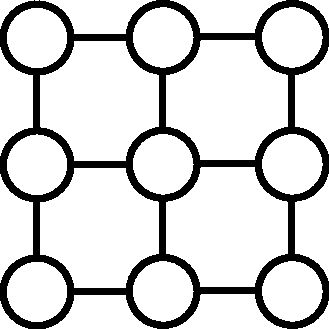
\includegraphics[height=0.2\paperheight]{fig/graphical-model-ising.pdf}
  \caption[Ising model as a probabilistic model]{
  \textbf{The Ising model is a probabilistic model used in statistical physics.} The nodes in this probabilistic graphical model represent random variables, and the edges in the graph represent relationships between neighboring random variables. In this Ising model there are nine random variables variables $\mbz = \{z_1, z_2, \ldots, z_9\}$ represented by nodes and the edges connecting two nodes indicate that those random variables interact in the energy function of the model $E(\mbz)$.}
  \label{fig:graphical-model-ising}
\end{figure}

\section{Probabilistic Models}
Probability models assign probability to configurations of random variables. The random variables in a probability model might correspond to observed variables in a physical system, or to latent properties representing patterns in data collected from the world, or a combination of both. To define a probability model, it is necessary to specify the density $p$ of a collection of random variables $\mbz$. We focus on probabilistic models $p(\mbz)$ where relationships between random variables can be encoded as edges in a graph, or  probabilistic graphical models~\citep{jordan2004graphical}.

\subsection{Example: Ising Model}
\label{sec:ising}
For example, consider a model used in statistical physics: the Ising model. The Ising model can be used to model interactions between atoms in a material~\citep{henelius2016refrustration} to study how the material behaves in different conditions, paving the way toward material design. This probabilistic model has binary random variables $z_n$ with density
\begin{equation}
  p(\mbz; \beta) = \frac{\exp(-\beta E(\mbz))}{\cZ}\, .
  \label{eq:boltzmann}
\end{equation}
The semicolon in \Cref{eq:boltzmann} denotes that the model has a parameter $\beta$, representing the reciprocal temperature of the system of random variables (a physical quantity). The energy function $E(\mbz)$ encodes the relationships between random variables, and $\cZ$, the normalizing constant, ensures that this probability distribution sums to one over all configurations of random variables~\citep{chandler1987introduction}. The energy function of the Ising model is\footnote{Bold letters can denote collections of random variables $\mbz = \{z_1, z_2,...,z_N\}$, or vectors, depending on the context.}
\begin{equation}
\label{eq:ising-energy}
  E(\mbz) = -\frac{1}{2}\sum_{i, j} J_{ij}z_i z_j - H\sum_i z_i\, .
\end{equation}
The interaction strength $J_{ij}$ defines the interactions between random variables. In a simple Ising model, only nearest neighbors interact, so $J_{ij}$ is nonzero if the random variables $z_i$ and $z_j$ are neighbors. The parameter $H$ increases or decreases the energy in proportion to the values of the random variables $z_i$; we give its physical interpretation later.

The Ising model can be represented as a probabilistic graphical model, shown in \Cref{fig:graphical-model-ising}. Two variables $z_i$ and $z_j$ interact (changing the value of one leads to a change in probability of the other) only if they share an edge in the graph. This representation works in conjuction with the density in \Cref{eq:boltzmann}, as the presence of an edge in the graph corresponds to two variables interacting in the energy function $E$. In this model, the energy function (and hence graph) is such that only neighboring random variables interact.

The Ising model can be used to study physical systems such as magnetic materials, where interactions between atoms can be encoded into the interaction strength $J_{ij}$. The interactions between random variables encoded in this manner contain the necessary information to model the properties of a material. In modeling a material, the random variables $\mbz$ can be referred to as spins. Spin is a type of angular momentum carried by particles comprising atoms, and such angular momentum causes a magnetic field. Although the random variables $\mbz$ are binary, taking on values of $-1$ and $+1$, they can be re-scaled to the magnetic strength of the atoms in a particular material of interest if comparison to experimental data is required. The parameter $H$ can be interpreted as the magnitude of an external magnetic field that interacts with the magnetic strength and orientation of every atom~\citep{chandler1987introduction}.

To see how well an Ising model mirrors a physical material, a property such as magnetization can be measured in the material, and calculated using the model. Magnetization is the average orientation of the magnetic strength of every atom or random variable in the material,
\begin{equation}
  M(\mbz) = \frac{1}{N}\sum_{i=1}^N z_i\, .
\end{equation}
By measuring the magnetization $M$ and computing its value in the Ising model, a practitioner can deduce how accurately the model reproduces experimental data. For example, if an Ising model with nearest neighbors ($J_{ij} \neq 0$ if $i$ neighbors $j$) does not accurately reproduce the magnetization of a physical material, it may be necessary to include second-nearest neighbor effects ($J_{ij}\neq 0$ if $i$ and $j$ are connected by a path of length at most two).

Another example of a quantity that can be measured experimentally and computed in a probabilistic model is the thermodynamic free energy $F$,
\begin{equation}
  \label{eq:free-energy}
  F = -\frac{1}{\beta} \log \cZ\, .
\end{equation}
The free energy of a system relates to the amount of energy that can be extracted from a system by its surroundings. For example, the free energy of a protein is used to understand its stability, and can be measured by the amount of energy needed to destroy its structure by denaturing it~\citep{stone2013the-theory}. In modeling a magnetic material or biological material, the free energy can be derived from the normalizing constant $\cZ$~\citep{chandler1987introduction}.

% !TEX root = ../main.tex
\newcommand\x{\scalebox{1.6}{\textbullet}}
\begin{table*}[t]
    \begin{center}
    \resizebox{0.9\textwidth}{!}{%
    \begin{tabular}{@{}lccccccccc|cccccc@{}}
      & \multicolumn{9}{c}{\bf Attributes} & \multicolumn{1}{c}{\bf                                                 User}\\
      \cmidrule(lr){2-10} \cmidrule(lr){11-15}
      {\bf Items} & Pizza & Eggs & Taco & Salad & Avocado & Chicken & Sardines & Beer & Coffee & 1  \\
      Morning Pizza & \x & \x & & & & & & & \x & \x \\
      Dinner Pizza & \x & & & & & & \x & \x & &   \\
      Small Salad & & & & \x & \x & & \x & & &  \\
      Big Salad & & \x & & \x & \x & \x & & & \x & \x  \\
      Taco & & & \x & & \x & \x & & & \x &  \\
      Fish Taco & & & \x & & & & \x & & &  \\
      \bottomrule
    \end{tabular}
    }
    \caption[Example binary classification data]{\label{tab:example-binary}Example binary classification data. A user consumes meals (rightmost column), and meals have attributes (table on the left. Meals are represented as datapoints $x_n$ with covariates being foods in the meals. The goal of a binary classifier trained on this data is to predict which meals a user will consume, or which datapoints $(x_n, y_n)$ have a label $y_n = 1$. An accurate classifier will information about which covariates are shared across positive or negative labeled datapoints; for example, this user consumes meals that include eggs and coffee.
    }
    \end{center}
\end{table*}
\subsection{Example: Binary Classification}
% !TEX root = ../main.tex
\begin{figure}[t]
  \centering
  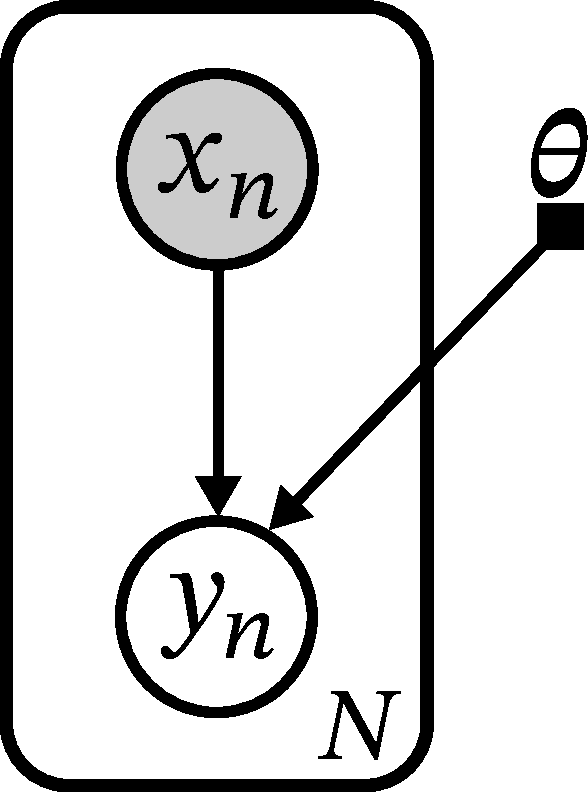
\includegraphics[height=0.2\paperheight]{fig/graphical-model-regression.pdf}
  \caption[Graphical model for logistic regression]{
  \textbf{Binary classification is a probabilistic modeling technique used in recommender systems.} Observed random variables are denoted by shaded nodes, and directed edges in the graph indicated conditional dependence on a node's parents. There are $N$ independent, identically distributed observations $(y_n, x_n)$; the rectangular plate denotes repetition of nodes and edges. The model predicts a binary response $y_n$ using parameters $\mbtheta$ and covariates $x_n$.}
  \label{fig:graphical-model-regression}
\end{figure}
Another example of a probabilistic model is a binary classifier~\citep{bishop2006pattern}, represented as a graphical model in \Cref{fig:graphical-model-regression}. Consider $N$ datapoints of the form $(x_n, y_n)$ consisting of covariates $x_n$ and binary responses $y_n$. As illustrated in \Cref{tab:example-binary}, the covariates $x_n$ might represent information about items such as foods in a meal, and $y_n$ may indicate whether a single user ate a meal with those foods. A binary classifier would then classify whether the user would eat a new meal $\hat{x}_n$ based on its constituent foods.

A binary classifier is defined using a regression function $f$ with parameters $\mbtheta$. The logistic function $\sigma$ applied to the regression function defines the probability model for a binary classifier,
\begin{equation}
  p(y_n \mid x_n; \mbtheta) = \frac{\exp\left( \sigma(f(x_n; \mbtheta)) \cdot y_n\right)}{\cZ}\, .
  \label{eq:binary-classification}
\end{equation}
The logistic function constrains the output of $f$ to the unit interval, and $\cZ$ is again the normalizing constant. The regression function $f$ uses information about a datapoint to classify whether the response $y_n$ is positive. An example of a regression function is an inner product, defined by
\begin{equation}
  f(x_n; \mbtheta) = \mbtheta^\top x_n\, ,
\end{equation}
which corresponds to logistic regression~\citep{bishop2006pattern}. Alternatively, a more flexible model can be built using a deep neural network~\citep{lecun2015deep}.
%A binary classifier can form the basis of a recommender system as we study in \Cref{ch:rfs}.

\section{Inference}
In a probability model, computing---or, inferring---properties of the probability distribution is a central task. One inference problem is to ascertain likely configurations of random variables. Another is to compute the sum of a probability distribution over a set of random variables, for example, to compute the normalizing constant~\citep{jordan2004graphical}.

\subsection{Computing Likely Configurations of Random Variables}
In the study of a probability model such as a binary classifier in \Cref{eq:binary-classification}, one question of interest is: for a set of observations $(x_n, y_n)$, what is a likely value of $\theta$? Maximum likelihood estimation is one way to answer this question~\citep{bishop2006pattern}.

A probability distribution like $p(\mby \mid \mbx; \mbtheta)$ is also known as a likelihood function. It defines the likelihood of a random variable $\mby$ conditional on the value of data $\mbx$, with the current setting of the parameters $\mbtheta$. The maximum likelihood estimate of the parameters of this probability model for the data $(\mbx, \mby)$ is given by
\begin{equation}
  \mbtheta^* = \argmax_{\mbtheta} p(\mby \mid \mbx; \mbtheta)\, .
\end{equation}
This maximum likelihood estimate of the parameters $\mbtheta^*$ can be computed using stochastic optimization if the data is large~\citep{robbins1951a-stochastic}. % what if the argmax is intractable, or an integral? #todo details

\subsection{Computing the Normalizing Constant}

The second central inference task in probabilistic modeling is summing a probability model over a set of random variables. One example of this is computing the normalizing constant $\cZ$. This inference problem requires computing a sum: the normalizing constant ensures a probability distribution sums to $1$ over values the random variables can take.

Consider computing the normalizing constant for the binary classifier in \Cref{eq:binary-classification}.  To compute the normalizing constant $\cZ$ for this probability model, we can sum over the binary values the random variable $y_n$ can take,
\begin{align}
1 &= \sum_{y_n \in \{0, 1\}} \frac{\exp\left( \sigma(f(x_n; \mbtheta)) \cdot y_n\right)}{\cZ} \\
\Rightarrow \cZ &= \sum_{y_n \in \{0, 1\}} \exp\left( \sigma(f(x_n; \mbtheta) \cdot y_n)\right)\\
\cZ &= 1 + \exp\left( \sigma(f(x_n; \mbtheta))\right)\, .
\end{align}
Inference of the normalizing constant $\cZ$ is straightforward in this probability model. The random variable $y_n$ is binary, so there are only two terms in the sum needed to compute the normalizing constant.

Next, consider computing the normalizing constant or partition function for the Ising model in \Cref{eq:boltzmann}. The random variables $z_n$ in this model also take on binary values. The partition function is computed by summing over all the values associated with all random variables in the system, $\mbz = \{z_1, \ldots, z_N\}$:
\begin{align}
1 &= \sum_{z_1 \in \{-1, +1\}} \ldots \sum_{z_N \in \{-1, +1\}} \frac{\exp(-\beta E(\mbz))}{\cZ}\\
\Rightarrow \cZ &= \sum_{z_1 \in \{-1, +1\}} \ldots \sum_{z_N \in \{-1, +1\}} \exp(-\beta E(\mbz))\, .
\label{eq:intractable-partition}
\end{align}
There are $N$ binary-valued random variables and $2^N$ terms in the sum required to compute the partition function, so inference in the Ising model is difficult. For Ising models used to study materials, the partition function is intractable to compute for most model sizes practitioners want to study and compare to physical realizations.

One way to address the issue of an intractable partition function is with sampling methods, such as Markov chain Monte Carlo~\citep{metropolis1953equation}. These algorithms enable inference by simulating likely configurations of random variables. These samples of likely configurations are used to approximate quantities of interest such as the partition function. But, Markov chain Monte Carlo methods are difficult to scale to probabilistic models with large numbers of correlated random variables. In this thesis, we instead use variational inference, an approximate inference algorithm that relies on optimization instead of sampling.
% Calculating the partition function can be difficult, and there are many ways around computing the partition function. For example, sampling methods and variational methods can be used to approximate properties of distributions such as properties derived from the partition function. Markov chain Monte Carlo~\citep{metropolis1953equation} allows sampling system configurations from the Boltzmann distribution of a model; these samples can be used to approximate physical quantities. Variational inference relies on optimizing (varying) functionals to derive approximations of distributions of interest, these approximations can be used to compute properties of a model. Variational inference has roots in mean field methods in physics~\citep{saul1996mean,hoffman2013stochastic,blei2017variational} as described in \Cref{ch:background}.

\section{Variational Inference}
% !TEX root = ../main.tex
\begin{figure}[t]
  \centering
  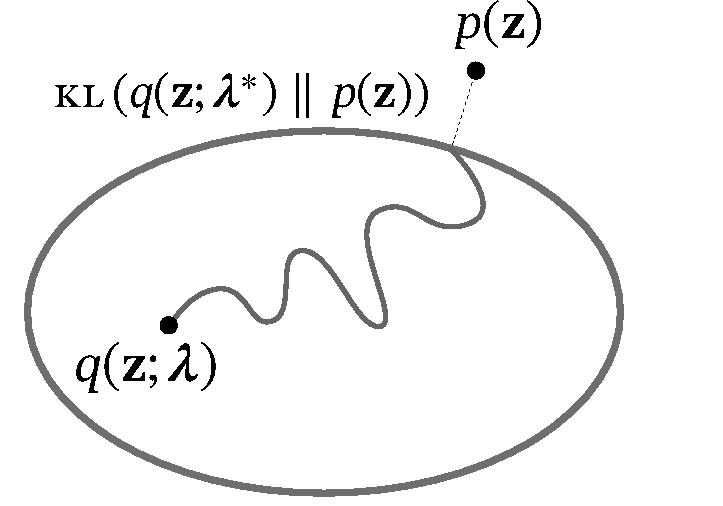
\includegraphics[height=0.2\paperheight]{fig/vi-cartoon.pdf}
  \caption[Variational inference cartoon]{
  \textbf{Variational inference finds the member of the variational family closest to the target distribution.} The oval in the cartoon represents the space of variational approximations $q(\mbz; \mblambda)$, and the goal of \acrlong{vi} is to find variational parameters $\mblambda^*$ that yield an approximation close to the target probability model $p(\mbz)$. One way to measure the distance between a variational approximation and the target probability distribution is with the \gls{kl} divergence.}
  \label{fig:vi-cartoon}
\end{figure}
Instead of working with a probability model $p(\mbz)$ directly, \acrfull{vi} posits a family of distributions $q(\mbz; \mblambda)$ indexed by parameters $\mblambda$~\citep{blei2017variational}. The goal of \gls{vi} is to find the closest member of the variational family $q$ to the target distribution $p$. The algorithm consists of varying the parameters $\mblambda$ to improve the quality of the approximation, as illustrated in \Cref{fig:vi-cartoon}. One way to measure the distance between the variational approximation and the target distribution is with the \acrfull{kl} divergence, or relative entropy~\citep{mackay2003information,ranganath2018black}.

The intractable partition function in $p(\mbz)$ appears in the \gls{kl} divergence \gls{vi} uses to assess distance,
\begin{equation}
\label{eq:kl}
    \KL{q(\mbz; \mblambda)}{p(\mbz)} = \E_q[\log q(\mbz ; \mblambda)] -\E_q[\log p(\mbz)] \\
\end{equation}
But it is possible to derive an objective function that does not depend on the partition function, starting from the \gls{kl} divergence. Taking the Ising model in \Cref{eq:boltzmann} as an example,
\begin{align}
  \KL{q(\mbz; \mblambda)}{p(\mbz)} &= \E_q[\log q(\mbz ; \mblambda)] -\E_q[\log p(\mbz)] \\
 \KL{q(\mbz; \mblambda)}{p(\mbz)} &= \E_q[\log q(\mbz ; \mblambda)] -\E_q[-\beta E(\mbz) - \log \cZ] \\
 \log \cZ &= \E_q[-\beta E(\mbz)] - \E_q[\log q(\mbz ; \mblambda)] + \KL{q(\mbz; \mblambda)}{p(\mbz)} \label{eq:second-last}  \\
 \Rightarrow \log \cZ \geq \cL(\mblambda) &\coloneq  \E_q[-\beta E(\mbz)] - \E_q[\log q(\mbz ; \mblambda)]\, .
 \label{eq:llbo}
\end{align}
This lower bound $\cL$ on the log normalizing constant is also called the \acrfull{elbo}, and serves as the objective function for \gls{vi}. In deriving this lower bound from \Cref{eq:second-last} to \Cref{eq:llbo}, we used the fact that the \gls{kl} is greater than or equal to zero. To show this fact, we start from Jensen's inequality for a convex function $f$, or
\begin{equation}
  f(\E[\mbz]) \leq \E[f(\mbz)]\, .
\end{equation}
The logarithm in the \gls{kl} is concave, so its negative is convex. We apply Jensen's inequality to the negative \gls{kl} in \Cref{eq:kl}:
\begin{align}
  -\KL{q(\mbz)}{p(\mbz)} &= \E_q\left[\log \frac{p(\mbz)}{q(\mbz )}\right] \\
  &\leq \log \E_q\left[\frac{p(\mbz)}{q(\mbz )}\right]\\
  &= \log \int  q(\mbz) \frac{p(\mbz)}{q(\mbz )}d\mbz \\
  &= \log \int  p(\mbz)d\mbz \\
  &= 0 \, .
\end{align}
This shows that the \gls{kl} is greater than or equal to zero~\citep{cover2012elements}.

The left-hand-side in \Cref{eq:llbo} does not change as the variational parameters $\mblambda$ are varied in $\cL(\mblambda)$. In words, maximizing the lower bound $\cL(\mblambda)$ is equivalent to minimizing the \gls{kl} divergence between the variational approximation and target probability model.

\subsection{Example: Mean Field Variational Inference in the Ising model}
\label{sec:ising-mean-field}

To demonstrate \gls{vi}, we use the Ising model described in \Cref{sec:ising} with probability distribution $p(\mbz)$ defined in \Cref{eq:boltzmann} and energy function $E(\mbz)$ in \Cref{eq:ising-energy}. Inspecting the intractable partition function of the Ising model can help construct a variational family $q(\mbz; \mblambda)$ to approximate the Ising model.

The Ising model partition function in \Cref{eq:intractable-partition} is intractable because the sums do not decompose by random variables: every sum must be carried out in order, because the result of the $N$th sum over the random variable $z_N$ depends on the results of the sums over the previous $N-1$ random variables. This is because of interactions between dependent random variables. The first term in the energy function of the Ising model represents nearest neighbor interactions, $z_iz_j$, and is graphically equivalent to the links between nearest neighbors in \Cref{fig:graphical-model-ising}.

However, the second term in the Ising energy function in \Cref{eq:ising-energy}, $H\sum_i z_i$, does decompose by random variable. Physically, this corresponds to a magnetic field applied to the system as a whole, so every random variable is subject to the same force. Mathematically, there is an outer sum over every configuration of random variables, and in this term the results of the summation over a variable $z_i$ do not affect the summation over another variable $z_j$. So this magnetic field term can be evaluated for systems with many random variables.

% !TEX root = ../main.tex
\begin{figure}[t]
  \centering
  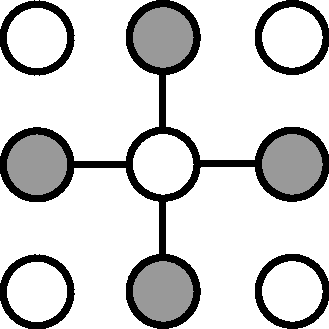
\includegraphics[height=0.2\paperheight]{fig/ising-markov-blanket.pdf}
  \caption[Markov blanket of a node in an Ising model]{
  \textbf{The structure of an Ising model can inform variational approximations.} This graphical model illustrates a Markov blanket in the Ising model of \Cref{fig:graphical-model-ising}. The Markov blanket of a node is the set of nodes whose values need to be fixed to render a node independent of the rest of the graph. In an Ising model, only neighboring random variables interact and therefore comprise the Markov blanket of a node. Here, the Markov blanket of the central node are shaded, indicating that their values are fixed. The missing edges between the peripheral nodes indicate that the central node is independent of the rest of the graph, conditional on its Markov blanket.}
  \label{fig:ising-markov-blanket}
\end{figure}
The structure of the Ising model energy function and corresponding graphical model can be used to build a variational approximation $q(\mbz; \mblambda)$ as follows. If the second term of the Ising model energy function does not lead to an intractable partition function due to every random variable being subject to a magnetic field, one can construct a variational approximation by extending this physical intuition and developing the concept of a `mean field'. Consider the central random variable $z_i$ in \Cref{fig:graphical-model-ising}. Fixing the values of its nearest neighbors renders this random variable independent of the rest of the graph as shown in \Cref{fig:markov-blanket-ising}. The nearest neighbors of the central random variable can then be interpreted as giving rise to a magnetic field. The strength of this magnetic field is unknown, so we can define this unknown strength as a variational parameter $\delta H$ that we will infer using \gls{vi}. This mean field is additive to the external magnetic field $H$ applied to the system as a whole, so the energy function for the central random variable $z_i$ under this mean field assumption can be written
\begin{equation}
  E_{\mf}(z_i; \delta H) = \delta H z_i + H z_i\, .
\end{equation}
Note that we have replaced the interaction term $J_{ij} z_iz_j$ in the Ising model energy function in \Cref{eq:ising-energy} by the mean field $\delta H$. The mean field assumption is that term can approximate the effects of neighboring nodes~\citep{chandler1987introduction}. If we repeat this argument for every node in the graph, we arrive at the mean field energy function
\begin{equation}
  E_{\mf}(\mbz; \delta H) = -(H + \delta H)\sum_{i = 1}^N z_i\, .
  \label{eq:mean-field-energy}
\end{equation}
The above construction starting from the mean field assumption corresponds to the variational approximation with density
\begin{equation}
  q(\mbz; \beta, \delta H) = \prod_{i=1}^N\frac{\exp(- \beta E_\mf(z_i; \delta H))}{\cZ_\mf} \, ,
  \label{eq:mean-field-distribution}
\end{equation}
and we see that the variational parameter $\mblambda$ is simply the mean field strength $\delta H$. The mean field variational approximation corresponds to a fully factorized probability distribution where every random variable is independent~\citep{wainwright2008graphical}. This is a useful property, as the partition function is tractable in this mean field variational approximation: we can compute the partition function for every random variable by itself. The partition function for a single random variable $z_i$ under the mean field assumption is straightforward,
\begin{align}
  \cZ_\textrm{\mf, i} &= \sum_{z_i \in \{-1, +1\}} \exp(- \beta (H + \delta H) z_i) \\
  &= 2 \cosh (\beta (H + \delta H)) \, ,
  \label{eq:partition-function-i}
\end{align}
and the partition function for the variational approximation for all variables is simply $\cZ_\mf = \cZ_\textrm{\mf, i}^N$. Similarly, the average of a random variable under the variational distribution is readily computed as
\begin{align}
\begin{split}
  \E_{q(z_i)}[z_i] &= \sum_{z_i \in \{-1, +1\}} \frac{z_i \exp(- \beta E_\mf(z_i; \delta H))}{\cZ_\textrm{\mf, i}} \\
 &= \sum_{z_i \in \{-1, +1\}} \frac{z_i \exp(- \beta (H + \delta H) z_i)}{2 \cosh(\beta (H + \delta H))} \\
 &= -\tanh(\beta (H + \delta H))\, .
 \label{eq:mf-mean}
 \end{split}
\end{align}
Now that we have constructed a variational family for the Ising model, we can proceed with the \gls{vi} algorithm. The next step is writing down and maximizing the lower bound on the log partition function to minimize the \gls{kl} between our approximating distribution and model.

The lower bound on the log partition function $\cL(\delta H)$  in \Cref{eq:llbo} becomes
\begin{align}
  \cL(\delta H) &= \E_q[-\beta E(\mbz)] - \E_q[\log q(\mbz; \delta H)] \\
  &= \E_q\left[-\frac{1}{2}\beta\sum_{i, j} J_{ij}z_i z_j - \beta H\sum_i z_i\right] - \E_q\left[ -\beta (H + \delta H)\sum z_i\right] + \log \cZ_{\mf} \\
  &= \E_q\left[-\frac{1}{2}\beta\sum_{i, j} J_{ij}z_i z_j + \beta\delta H\sum_i z_i\right] + \log \cZ_{\mf}\, ,
\intertext{and we can take the expectation inside the sum using the fact that the mean field variational distribution is fully factorized, so }
  \cL(\delta H) &= -\frac{1}{2}\beta \sum_{i, j}J_{ij}\E_{q(z_i)}[z_i]\E_{q(z_j)}[z_j] + \beta \delta H \sum_i \E_{q(z_i)} [z_i] + \log \cZ_{\mf}\, .\\
\end{align}
In the first term, recall that two random variables $z_i$ and $z_j$ have the same distribution under the mean field assumption, and that every variable interacts with its four nearest neighbors in the Ising model. The lower bound on the log partition function then becomes
\begin{align}
 \cL(\delta H) &= -\frac{1} {2} \beta 4JN \E_{q(z_i)}[z_i]^2 + \beta N \delta H \E_{q(z_i)} [z_i] + \log \cZ_{\mf}\, .
\end{align}
The next step in the \gls{vi} algorithm is maximizing this lower bound, to minimize the \gls{kl} divergence between the variational approximation and the model. Taking the derivative with respect to $\delta H$ and suppressing the subscript of the expectation operator, we get
\begin{align}
\frac{\partial\cL(\delta H)}{\partial \delta H} &= N\beta(-4J\E[z_i]\partial_{\delta H}\E[z_i] + \E[z_i] + \delta H \partial_{\delta H} \E[z_i]) + N\beta \tanh(\beta (H + \delta H))\, .
\end{align}
Next, setting this derivative to zero and cancelling out terms (and using \Cref{eq:mf-mean}) leads to
\begin{align}
 0 &= -4J\E[z_i]\partial_{\delta H}\E[z_i] + \delta H \partial_{\delta H} \E[z_i]) \\
 \Rightarrow \delta H \partial_{\delta H} \E[z_i]) &= 4J\E[z_i]\partial_{\delta H}\E[z_i] \\
 \Rightarrow \delta H^* &= 4J\E[z_i]\, .
\end{align}
This shows that under a mean field assumption, the variational parameter that maximizes the lower bound on the log partition function---and hence minimizes the \gls{kl} divergence between the approximation and model---is proportional to the mean field around any node in the system. The structure of the model informs our choice of variational approximation.

The quality of the variational approximation $q(\mbz; \beta, \delta H^*)$ from \gls{vi} can be assessed in several ways. For example, the magnetization $M$ or the free energy $F$ can be calculated using the variational approximation, and these values can be compared to Markov Chain Monte Carlo simulations in small systems. This can be viewed as a type of predictive check for a \gls{vi} algorithm~\citep{blei2014build}. However, the development of theoretical guarantees to assess the quality of variational approximations found with \gls{vi} is an open area of research~\citep{wang2019frequentist}. Practitioners must currently empirically evaluate the quality of variational approximations according to the task at hand, as we do in \Cref{ch:hvm,ch:pvi}.

\subsection{Variational Inference Originated in Statistical Physics}

Previously, we derived a variational approximation to the Ising model by making a mean field assumption. That the language of physics is used in machine learning algorithms such as \gls{vi} is no coincidence. In fact, \citet{feynman1972statistical,feynman2018statistical} derives the \gls{gbf} inequality for use in a variational principle for approximating intractable partition functions using mean field assumptions. Consider a model with energy function $E$ and partition function $\cZ$, and a mean field variational approximation with energy function $E_\mf$ (and corresponding partition function $\cZ_\mf$). Then the \gls{gbf} inequality reads~\citep{feynman1972statistical,feynman2018statistical}
\begin{equation}
\cZ \geq \cZ_\mf\exp\left(-\beta \braket{E - E_\mf}_\mf\right) \, .
\label{eq:gbf-inequality}
\end{equation}
In physics, bra-ket notation is used to denote expectations. For example, expectations with respect to \Cref{eq:mean-field-distribution} are written $\braket{\; \cdot \;}_\mf$. Rewriting the \gls{gbf} with statistics notation for the expectation $\E_q[\;\cdot\;]$ yields
\begin{align}
 \cZ &\geq \cZ_\mf\exp\left(-\beta \E_q[E - E_\mf]\right) \, .
\end{align}
Taking the logarithm, we recover the lower bound on the log partition function
\begin{align}
 \log \cZ &\geq \E_q[-\beta E] - \E_q[-\beta E_\mf] + \log \cZ_\mf\\
 &= \E_q[-\beta E] - \E_q[\log q_\mf(\mbz; \mblambda)] \\
 &= \cL(\mblambda)\, .
\end{align}
This is identical to the log partition function lower bound in \Cref{eq:llbo}. \citet{hoffman2013stochastic} review the historical roots of the variational principle in its machine learning incarnation.

To complete the connection to machine learning, we relate this log partition function lower bound to the evidence lower bound studied in the \gls{vi} literature~\citep{blei2017variational}. A probabilistic model of data might have the following process for generating data $\mbx$ using prior information in latent variables $\mbz$:
\begin{align*}
\mbz &\sim p(\mbz)\\
\mbx &\sim p(\mbx \mid \mbz)
\end{align*}
The posterior distribution of this model is computed using Bayes' rule,
\begin{equation*}
  p(\mbz \mid \mbx) = \frac{p(\mbx \mid \mbz) p(\mbz)}{p(\mbx)} \, .
\end{equation*}
The model evidence $p(\mbx)$ is the partition function of the posterior. Calculating the partition function is what makes posterior inference difficult, as it requires integration over the latent variables $\mbz$,
\begin{equation*}
  p(\mbx) = \int p(\mbx, \mbz) d\mbz \, ,
\end{equation*}
and the latent variables $\mbz$ are typically high-dimensional, such as the number of random variables in an Ising model. But \gls{vi} can be used to approximate this intractable integral. The lower bound on the log partition function becomes the \gls{elbo}:
\begin{align}
\log p(\mbx) &\geq \cL(\mblambda) \\
\cL(\mblambda) &= \E_q[\log p(\mbx, \mbz)] - \E_q[\log q(\mbz ; \mblambda)] \, .
\end{align}
An example of a latent variable model without data is the Ising model---in this case, the data is an empty set, $\mbx = \{\}$. In this case $\cL(\mblambda)$ is a lower bound on the log partition function as we derived in \Cref{eq:llbo} and identical to the \gls{gbf} inequality.
% \gls{vi} is an algorithm to find a good approximation to a target probability distribution that has an intractable integral, such as the sum needed to compute a partition function. We now turn to the second inference problem of computing likely configurations of variables in a probability model.

\section{Conclusion}
We reviewed probability models and gave examples of their use in statistical physics and recommender systems. The task of inference is central to working with probability models; we described variational inference and maximum likelihood estimation. The following chapters address the issue of building the structure of a problem into a performant probability model, whether that structure concerns the connectivity in a statistical physics model, the structure of datapoints in a recommender system, or information about a variational approximation useful in an optimization algorithm for this approximation.

% !TEX root = altosaar-2020-thesis.tex
\chapter{Hierarchical Variational Models for Statistical Physics}
\label{ch:hvm}
\lettrine[image=true,lines=3]{design/A}{s} probabilistic modeling finds widespread use in science, it is necessary to adapt machine learning tools to the specifics of a scientific domain. In this chapter we focus on probabilistic models used in statistical physics. Whether such models are used in molecular dynamics simulations for finding drug candidates for disease~\citep{shamay2018quantitative} or simulating solid state systems for materials design~\citep{schmidt2019recent}, the scalability of machine learning methods is a bottleneck for progress. Simulations need to be run for longer timescales and in larger systems, and must leverage knowledge about the physical system under study to yield accurate predictions. As a step in this direction, this chapter centers on building scalable variational approximations for statistical physics models, and develops hierarchical probabilistic models to study their performance in large statistical physics systems.
% !TEX root = ../main.tex
\section{Introduction}
In statistical physics, building a model corresponding to a physical system is useful: comparing how the model's predictions differ from experiment can be used to understand how a system behaves. For computing properties corresponding to a model's behavior, the normalization constant of the model's Boltzmann distribution in \Cref{eq:boltzmann} is a central quantity. The partition function can be used to derive properties of physics models that can be measured in experimental realizations, such as specific heat or magnetization. Such properties of models can be compared to experimental values, which can inform how a model might be improved to better mirror reality. But the partition function is intractable for many probabilistic models of interest, as described in \Cref{ch:background}.

One workaround to the problem of an intractable partition function is to use an approximate inference algorithm such as \gls{mcmc}. \gls{mcmc} relies on sampling likely configurations of a system and does not require calculating the partition function. In theory, these samples will be draws from the probability model of interest~\citep{metropolis1953equation,andrieu2003an-introduction}. For example, samples from the Boltzmann distribution can be used to approximate physical quantities derived from the probability model, such as specific heat.

However, with limited computation \gls{mcmc} has limitations. This method requires practitioners to use convergence diagnostics~\citep{brooks1998general} to assess whether samples from the algorithm are independent. Scalable \gls{mcmc} requires careful consideration. While some scalable versions of \gls{mcmc} have been developed~\citep{neal2011mcmc,welling2011bayesian}, they are biased samplers that may not have guaranteed convergence to samples from the probability model of interest. This is similar to how in \gls{vi} performance must often be assessed empirically. But in comparison to \gls{vi}, unless a model-specific algorithm has been developed~\citep{wolff1989comparison}, generic \gls{mcmc} methods do not readily scale to large numbers of random variables.
% - describe the contributions of our paper: (1) show that
% gibbs-bogoliubov-feynman inequality is equivalent to variational inference.
% (1) show how the reinforcement learning approach of wu (2019) is more
% naturally expressed in terms of variational inference. (2) show that a modern
% tool of variational inference, HVMs, is useful and improves on wu (2019) by
% scaling to larger system sizes.

In \Cref{ch:background} we showed that the machine learning framework of \gls{vi} is equivalent to the \acrlong{gbf} variational principle. This has allowed practitioners to study statistical physics models using many variational approximations, including \glspl{van}. As an example of a variational method enabled by \gls{vi}, we study \glspl{hvm} as approximations to the Boltzmann distribution of statistical physics models. We find that \glspl{hvm} scale to larger systems sizes than \glspl{van} in Sherrington-Kirkpatrick and Ising models. Testing the feasibility of \gls{vi} methods in statistical physics is a twofold opportunity. Statistical physics problems might serve as benchmarks for \gls{vi}, and using \gls{vi} for these problems can lead to improved computational methods in statistical physics. % and where exact solutions ar eknown?
\paragraph{Related Work.} The \gls{gbf} variational principle has been used to study Markov random fields~\citep{jun-zhang1996the-application} and the connection between variational inference and statistical physics has been well-documented~\citep{blei2017variational,hoffman2013stochastic,mackay2003information}. But this equivalence between \gls{vi} and the \gls{gbf} inequality might serve as an introduction to \gls{vi} for physicists. \citet{wu2019solving} implicitly use \gls{vi}, by developing \glspl{van} and a reinforcement learning policy gradient algorithm (however, \gls{vi} is not mentioned). Further, for a system of size $L$, autoregressive neural networks require $\cO(L^2)$ forward passes to sample a system configuration, making \glspl{van} intractable in larger systems. The use of \glspl{hvm} can be advantageous for statistical physics as these models can sample from a system in $\cO(L)$ time and yield results for larger systems.

\paragraph{Variational Inference.}
\gls{vi} is equivalent to the \gls{gbf} variational principle and requires similar choices of a practitioner. The variational family $q(\mbz; \mbnu)$ to approximate a model must be chosen, in addition to a method to maximize the variational lower bound in \Cref{eq:llbo}.

The \gls{vi} literature provides several choices of variational family, such as a mean field, factorized variational distribution with independent latent variables. Another choice of variational family is the Bethe approximation, which constrains the variational distribution to the polytope of mean parameters that captures correlations between any two latent variables~\citep{wainwright2008graphical}. Some machine learning research focuses on developing variational approximations that capture correlations between latent variables~\citep{hoffman2015stochastic,kingma2016improved,maaloe2016auxiliary,wu2019solving}. An example of a variational family that can model correlations between latent variables is the \gls{van} family~\citep{wu2019solving}, which uses autoregressive neural networks to parameterize the variational distribution ${q(\mbz_i \mid \mbz_1, \ldots, \mbz_{i-1})}$. We explore the \gls{hvm} class of variational approximations~\citep{ranganath2018black}.

The second choice required to employ \gls{vi} is how to optimize the variational lower bound in \Cref{eq:llbo}. The choice of variational family can limit the available optimization techniques. For a simple variational family like the mean field approximation, it may be possible to analytically evaluate the expectations in \Cref{eq:llbo}. Then derivatives of the variational bound with respect to the variational parameters $\mbnu$ and manual calculation can maximize the lower bound, as derived in \Cref{sec:ising-mean-field}. If more expressive variational families are used (e.g. \gls{van}s with thousands or millions of variational parameters), the analytic approach is infeasible. Stochastic optimization and automatic differentiation software have been used to develop several approaches to computing gradients of the variational lower bound, such as \acrlong{bbvi}~\citep{ranganath2018black,mohamed2019monte}.
% !TEX root = ../../main.tex
\newcommand{\mywidtht}{0.25\textheight}
\newcommand{\figwidtht}{0.3\textheight}
\begin{figure}[t]
  \centering
  % adjust margin to center captions
  \captionsetup[subfigure]{justification=centering,margin={0cm,0cm},oneside}
  \hfill%\hspace{\mywidtht}%
  \begin{subfigure}[b]{\figwidtht}
    \centering
    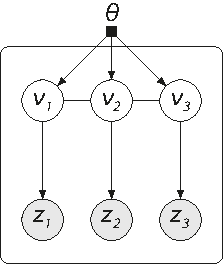
\includegraphics[width=\mywidtht]{ch-hvm/fig/hierarchical-variational-model.pdf}
    % \caption{\Acrlong{hvm}}%
    \label{fig:hvm-graphical-model}%
  \end{subfigure}
  \hspace*{\fill}%
  \begin{subfigure}[b]{\figwidtht}
    \centering
    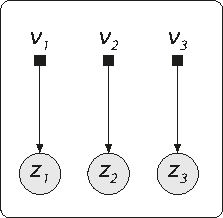
\includegraphics[width=\mywidtht]{ch-hvm/fig/mean-field-graphical-model.pdf}
    % \caption{Mean-field variational family}%
    \label{fig:mean field-graphical-model}%
  \end{subfigure}
  \hspace*{\fill}%
  % \vspace{-0.5cm}
  \caption[\textsc{hvm} and mean field approximation graphical models]{\textbf{\Acrlongpl{hvm} (\glspl{hvm}, left) capture dependencies between latent variables, compared to the mean field variational family with independent variables (right).}}
  \label{fig:graphical-model}
\end{figure}

The choice of variational family $q(\mbz; \mbnu)$ and optimization method for maximizing the variational lower bound leads to a trade-off intrinsic to \gls{vi}. Simple variational approximations such as the mean field family may be computationally feasible but inaccurate. The cost of increased accuracy, say by using a structured variational approximation, is increased computation. We illustrate the use of \gls{vi} in statistical physics by comparing two choices of variational approximation, \glspl{hvm}~\citep{ranganath2018black} and \glspl{van}~\citep{wu2019solving}. Many other variational approximations can be explored in future work.

% !TEX root = ../main.tex
\section{Hierarchical Variational Models}
For studying models with correlated random variables, such as frustrated spin systems~\citep{zdeborova2016statistical}, unstructured variational families such as the mean field are insufficient. \Acrfullpl{hvm} are one way to model correlated latent variables. An \gls{hvm} is defined by placing a `variational prior' on the variational parameters $\mbnu$ of the mean field variational family, in analogy to hierarchical probabilistic models. By leveraging neural networks to parameterize the variational prior, \glspl{hvm} can capture complex dependencies between random variables~\citep{ranganath2018black}.

% !TEX root = ../../main.tex
\begin{figure}[t!]
  \centering
  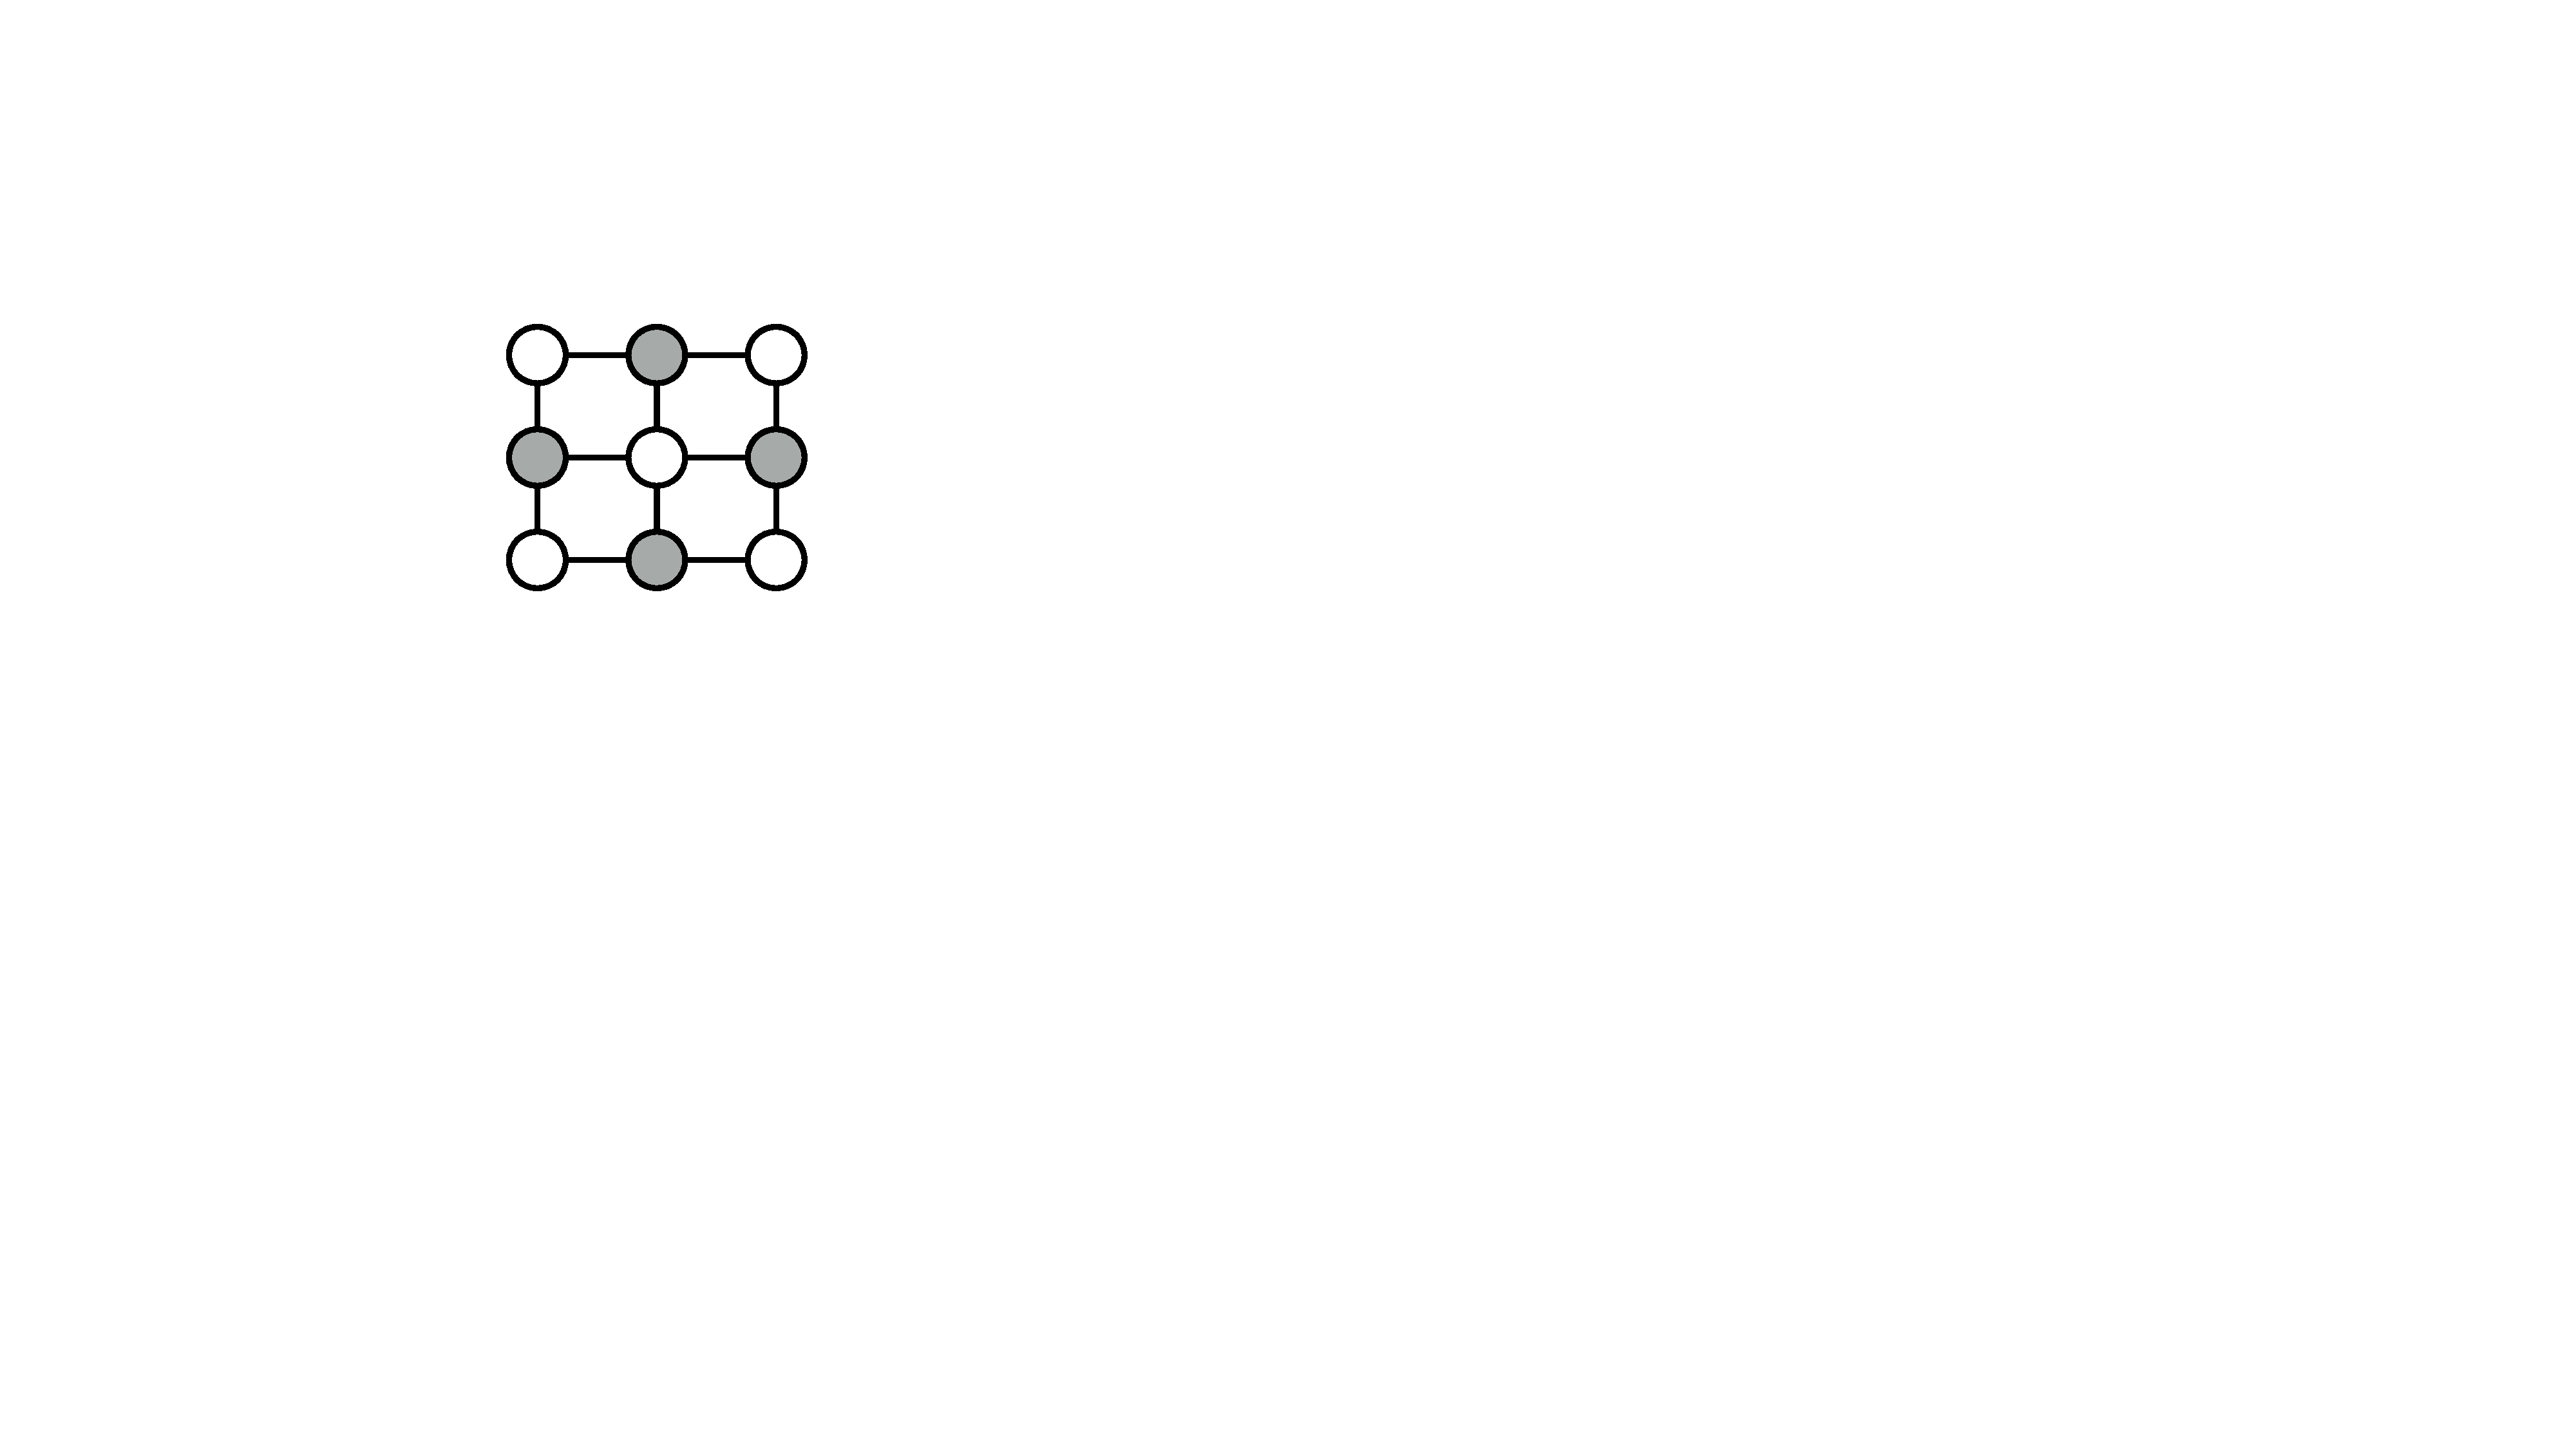
\includegraphics[height=0.2\paperheight]{ch-hvm/fig/markov-blanket-ising.pdf}
  \caption[Markov blanket of a random variable in an Ising model]{
  \textbf{The Markov blanket of a node in an Ising model consists of the node's nearest neighbors (nodes in the Markov blanket of the central node are shaded).} Conditioning on the Markov blanket of a node in a graphical model renders it conditionally independent of the rest of the variables. This enables building efficient variational approximations.}
  \label{fig:markov-blanket-ising}
\end{figure}

For studying a model $p(\mbx, \mbz)$, the variational family defined by an \gls{hvm} is defined as
\begin{equation}
  q_\hvm(\mbz; \mbtheta) = \int q(\mbnu; \mbtheta) \prod_i q(\mbz_i \mid \mbnu_i) d\mbnu \, ,
  \label{eq:hvm}
\end{equation}
where $q_\mf(\mbz \mid \mbnu) = \prod_i q(\mbz_i \mid \mbnu_i)$ is the mean field `variational likelihood' with parameters $\mbnu$, and $q(\mbnu; \mbtheta)$ is the variational prior with parameters $\mbtheta$. \Cref{fig:graphical-model} shows the graphical model for \glspl{hvm} as compared to the mean field family graphical model.

To use an \gls{hvm} in \gls{vi}, the variational lower bound must be optimized. But the variational lower bound in \Cref{eq:llbo} requires calculating the entropy of the variational distribution, and such integration in high dimensions can be intractable. As detailed in \citet{ranganath2018black}, the entropy can be lower-bounded by introducing an auxiliary `variational posterior' distribution $r(\mbnu \mid \mbz; \mbphi)$ with parameters $\mbphi$. This leads to the hierarchical evidence lower bound,
\begin{equation}
  \widetilde{{\cL}}(\mbtheta, \mbphi) = \E_{q(\mbz, \mbnu; \mbtheta)}[ \log p(\mbx, \mbz) + \log r(\mbnu \mid \mbz; \mbphi) - \log q(\mbz \mid \mbnu) - \log q(\mbnu; \mbtheta)]\, ,
  \label{eq:hier-elbo}
\end{equation}
and a stochastic optimization algorithm for this objective is developed in \citep{ranganath2018black}. \gls{vi} with an \gls{hvm} requires specifying the variational prior $q(\mbnu; \mbtheta)$ and the variational posterior ${r(\mbnu \mid \mbz; \mbphi)}$, then optimizing the hierarchical \gls{elbo} in \Cref{eq:hier-elbo}.

\paragraph{Specifying an \gls{hvm} with Normalizing Flows.} We study several choices of variational prior and recursive variational posterior. One choice of variational prior $q(\mbnu; \mbtheta)$ is an inverse autoregressive flow~\citep{kingma2016improved}. If the variational posterior $r(\mbnu \mid \mbz; \mbphi)$ is chosen to be a masked autoregressive flow~\citep{papamakarios2017masked}, the analytical forms of these flows are equivalent. These choices lead to a complexity of $\cO(L)$ for sampling latent variables in a system of size $L$. (This is because the noise used to sample from the variational prior can be drawn in parallel.) \glspl{hvm} should therefore be faster than \gls{van} approximations in large systems: the autoregressive requirement in \glspl{van} leads to a complexity of $\cO(L^2)$. A research question is whether the advantage in speed of \glspl{hvm} leads to a drop in accuracy that is too large to answer a statistical physics question.
% !TEX root = ../../main.tex
\begin{figure*}[t]
  \centering
  % adjust margin to center captions
  \captionsetup[subfigure]{margin={0cm,0cm},oneside}
  \hspace*{\fill}%
  \begin{subfigure}[c]{0.5\linewidth}
    \centering
    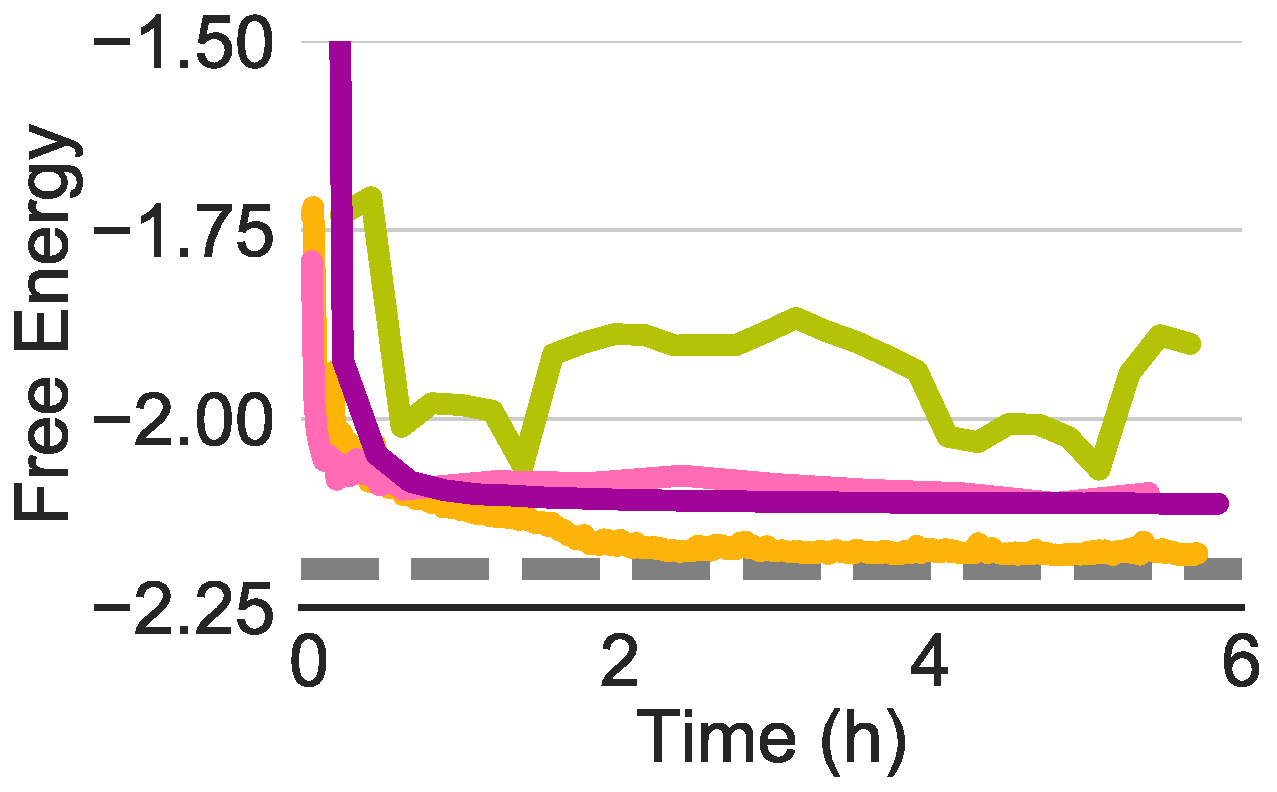
\includegraphics[width=\textwidth]{ch-hvm/fig/ising-large.pdf}
    % \caption{$\beta=0.4$}%
  \end{subfigure}
  % \hfill\hspace{\mywidth}%
  \begin{subfigure}[c]{0.3\linewidth}
    \centering
    % \raisebox{12mm}{
      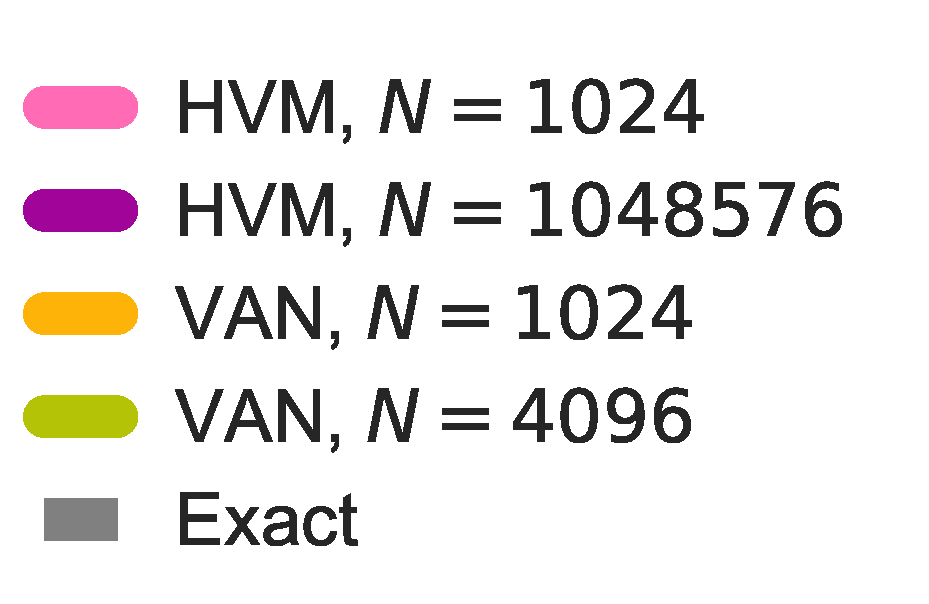
\includegraphics[width=\textwidth]{ch-hvm/fig/legend-ising}
    % }
  \end{subfigure}
  \hspace*{\fill}%
  % \vspace{-0.5cm}
  \caption[\textsc{hvm}s applied to the Ising model]{\textbf{\Acrfullpl{hvm} scale to statistical physics models with millions of random variables, with over 100x parameter savings.} The free energy is reported (the variational lower bound yields an upper bound on the free energy). The \gls{hvm} variational approximations use $5400$ parameters, while the \gls{van} method uses over $700$k.}
  \label{fig:hvm-ising}
\end{figure*}

\paragraph{Scalable \glspl{hvm} using Ising Model Structure.} Although \glspl{hvm} with autoregressive flows scale linearly, such variational approximations do not leverage the structure about the statistical physics under study. For example, it is difficult to index random variables so that nearest neighbors are grouped together when fed to an autoregressive model. However, consider the Markov blanket of a random variable in the Ising model---it contains all the information needed to render a variable conditionally independent of the rest of the model. The Markov blanket of a node in an Ising model consists of a node's nearest neighbors and is shown in \Cref{fig:markov-blanket-ising}. This means that an autoregressive model is overparameterized. For example, the last variable to be fed to the model depends on all the previous in an autoregressive model, whereas an efficient model might only consider nodes in a Markov blanket. A convenient way to build this structure into an \gls{hvm} would ensure efficient use of information from nearest neighbors in the Ising model. One way to formalize this problem structure is with convolutional neural networks~\citep{lecun2015deep}. We parameterize the variational prior and recursive posterior with \gls{realnvp} transformations using a convolutional neural network architecture \citep{dinh2017density}. Specifically, we parameterize the convolutional kernels to mimic the Markov blanket shown in \Cref{fig:markov-blanket-ising}: for every node, only its nearest neighbors are conditioned on.
% !TEX root = ../main.tex
\section{Empirical Study}
\label{sec:hvm-experiments}
% !TEX root = ../main.tex
\begin{figure*}[t]
  \centering
  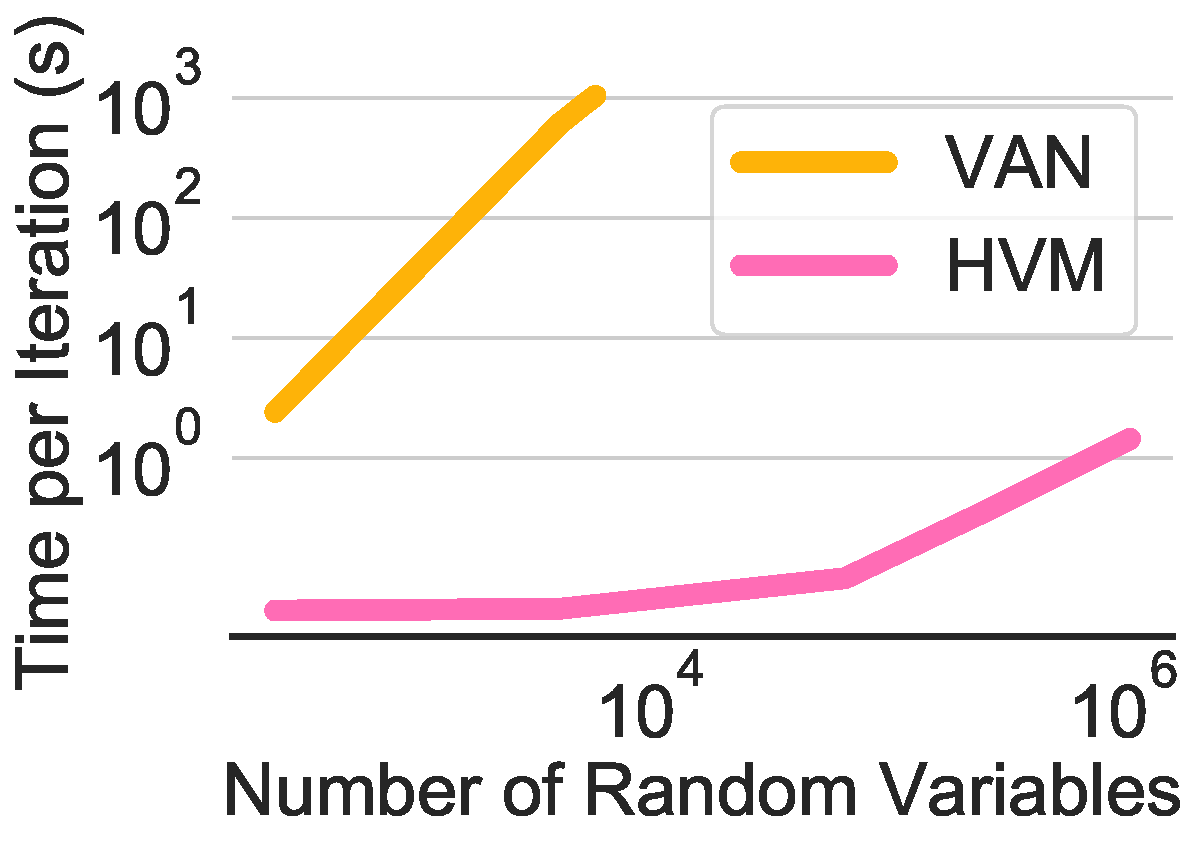
\includegraphics[width=0.5\textwidth]{fig/ising-scaling.pdf}
  \caption[Comparing scaling of \textsc{hvm}s to \textsc{van}s in large systems]{\textbf{\Acrfullpl{hvm} are faster than \Acrfullpl{van} \citep{wu2019solving} and scale to larger systems.} The scaling of both variational approximations is illustrated with the time taken per iteration in Ising models. The \gls{hvm} variational approximations use $5400$ parameters and the \gls{van} method uses over $700$k. The \gls{van} approximation runs out of memory with $16384$ random variables, while the \gls{hvm} method scales to models with over $1$M random variables.}
  \label{fig:ising-scaling}
\end{figure*}
To study the utility of \gls{vi} tools for statistical physics systems, we compare \glspl{hvm} to \gls{van} approximations~\citep{wu2019solving}.\footnote{Code is available at \url{https://github.com/altosaar/hierarchical-variational-models-physics}.} We use the same benchmarks as in \citet{wu2019solving}: the models of Ising and Sherrington-Kirkpatrick. We evaluate variational inference methods by assessing whether they lead to lower estimates of the free energy of a model. (Lower is better, as the free energy in  \Cref{eq:free-energy} is proportional to the negative of the variational lower bound in \Cref{eq:llbo,eq:hier-elbo}.)

\paragraph{Experimental Setup.} To assess whether \glspl{hvm} outperform \glspl{van} in large systems, the computational budget for the \gls{vi} algorithm using both variational approximations was set to 6~hours.  All experiments were performed on NVIDIA Tesla P100 GPUs, and the reference implementation of \glspl{van} released in \citet{wu2019solving} was used. \gls{van} models were unable to complete sufficiently many iterations in the allocated compute time, so all experiments were run without annealing the temperature of the system. For calculating the free energy using \glspl{hvm}, importance sampling~\citep{owen2013monte} was used with an \gls{hvm} as the proposal (for \glspl{van}, the increased cost of sampling prohibited drawing enough samples for low-variance importance sampling estimates, so Monte Carlo estimation was used). In \glspl{hvm}, variational approximations that accounted for problem structure using \gls{realnvp} transformations outperformed autoregressive parameterizations, and we omit these results.

\paragraph{Ising Model.} For small systems, \glspl{hvm} were more accurate than \gls{van} models at lower temperatures; at higher temperatures (such as the critical temperature), \gls{van} models were slightly more accurate. This could be because annealing was not used to fit \gls{van} models, and the randomness of the hierarchical latent variables in \glspl{hvm} obviates the need for annealing. In large systems (e.g. $L=128$), \gls{van} models failed to complete a single iteration, while \glspl{hvm} were able to complete many iterations (at the cost of some accuracy). The trade-off between model size and computational cost was significant between autoregressive choices of variational approximations in \glspl{hvm} versus \gls{realnvp} convolutional approximations. \Cref{fig:hvm-ising} shows that convolutional models were able to scale to models with over a million random variables, with only a slight decrease in accuracy relative to \gls{van} methods, and with $100$ times fewer parameters. This is also illustrated via the time per iteration for both a \gls{van} and \gls{hvm} variational approximation reported in \Cref{fig:ising-scaling}.

% !TEX root = ../../main.tex
\newcommand{\mysize}{0.2\textheight}
\newcommand{\mywidth}{0.1\linewidth}
\newcommand{\figwidth}{0.5\linewidth}
\begin{figure*}[t]
  \centering
  % adjust margin to center captions
  \captionsetup[subfigure]{margin={0cm,0cm},oneside}
  \hspace*{\fill}%
  \begin{subfigure}[c]{0.5\linewidth}
    \centering
    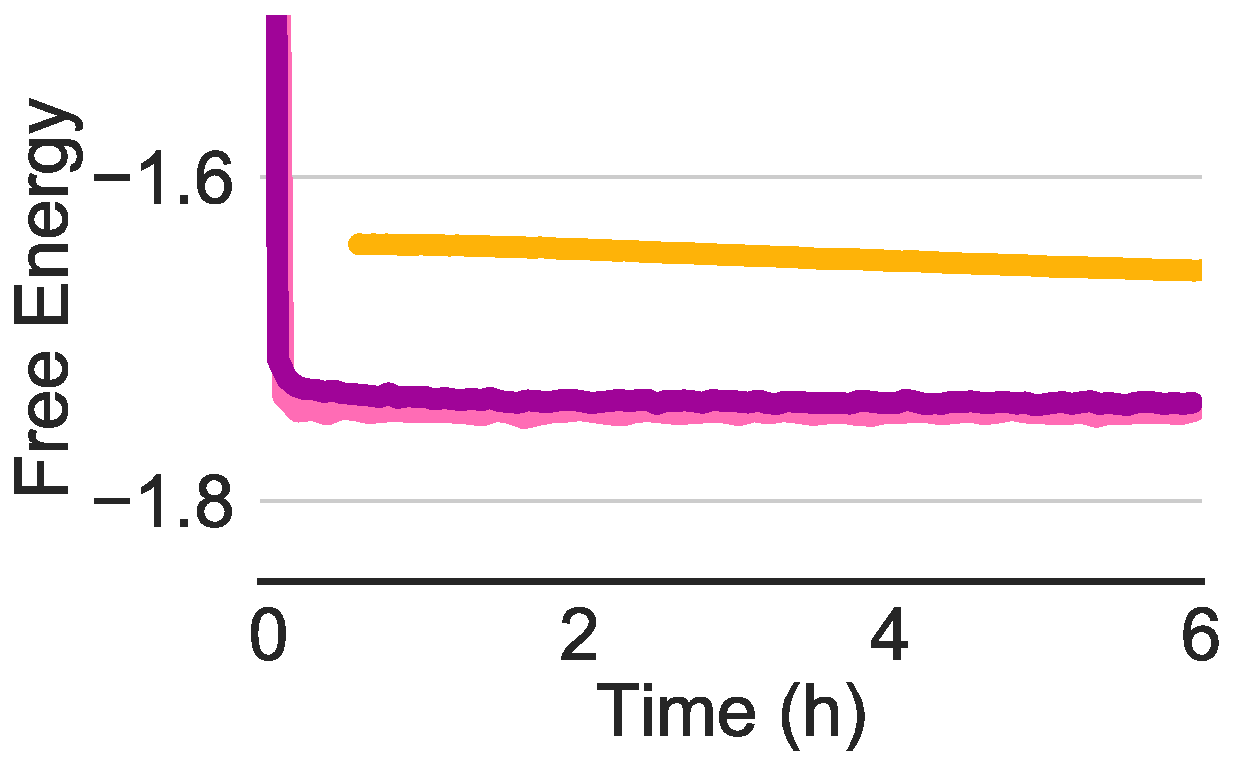
\includegraphics[width=\textwidth]{ch-hvm/fig/sk-large.pdf}
    % \caption{$\beta=0.4$}%
  \end{subfigure}
  % \hfill\hspace{\mywidth}%
  \begin{subfigure}[c]{0.3\linewidth}
    \centering
    % \raisebox{12mm}{
      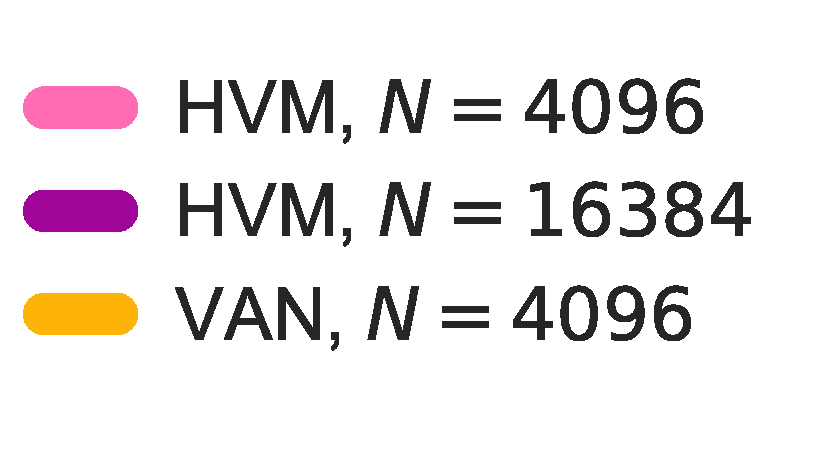
\includegraphics[width=\textwidth]{ch-hvm/fig/legend-sk}
    % }
  \end{subfigure}
  \hspace*{\fill}%
  % \vspace{-0.5cm}
  \caption[\textsc{hvm}s applied to the Sherrington-Kirkpatrick model]{\textbf{\Acrfullpl{hvm} scale to larger systems than \acrfull{van} models \citep{wu2019solving} when fit to the Sherrington-Kirkpatrick model using \acrlong{vi}.} (Lower is better, as the variational lower bound yields an upper bound on the free energy.) For the system with $N=4096$ variables the \gls{van} method completed fewer than ten iterations, and with $N=16384$ did not complete a single iteration.}
  \label{fig:sk}
\end{figure*}

\paragraph{Sherrington-Kirkpatrick Model.} The free energy estimates using \gls{vi} with either \gls{hvm} or \gls{van} approximations are plotted in \Cref{fig:sk} for the Sherrington-Kirkpatrick model. \gls{hvm} approximations outperformed \gls{van} approximations, and scaled to larger systems where the $\cO(L^2)$ cost of sampling from a \gls{van} prohibited even a single iteration.

\section{Discussion}
The \gls{gbf} inequality holds for quantum systems~\citep{feynman1972statistical,feynman2018statistical}, and  applying \gls{vi} and \glspl{hvm} to quantum systems is a direction for future work. Physics tools (such as \gls{vi} in its original incarnation) have been useful in machine learning~\citep{bamler2017perturbative}, and we hope the reverse holds---that tools from machine learning such as \gls{vi} and \glspl{hvm} continue to find use in statistical physics. Further scaling \glspl{hvm} to statistical physics models where system size is a bottleneck is a goal of future work, especially in settings relevant to medicine, such as in protein folding or drug screening problems.

% !TEX root = altosaar-2020-thesis.tex
\chapter{RankFromSets: Scalable Set Recommendation with Optimal Recall}
\label{ch:rfs}
\lettrine[image=true,lines=3]{design/I}{n} the previous chapter, we built scalable and performant probabilistic models of likely configurations of interacting atoms in statistical physics systems. Modeling choices were guided by the structure of the underlying patterns of interaction between random variables. As another case study, we turn to recommender systems in this chapter, where the core problem is to model which items a user is likely to interact with. By building the structure of individual datapoints into a probabilistic model of user interaction, and considering the goals of the recommendation task, we develop a scalable, accurate framework for recommending items with attributes.
% !TEX root = ../main.tex
\section{Introduction}\label{sec:rfs-introduction}
% !TEX root = ../../main.tex
% \newcommand\x{\scalebox{1.6}{\textbullet}}
\begin{table*}[t]
    \begin{center}
    \resizebox{1.0\textwidth}{!}{%
    \begin{tabular}{@{}lccccccccc|cccccc@{}}
      & \multicolumn{9}{c}{\bf Attributes} & \multicolumn{5}{c}{\bf                                                 Users}\\
      \cmidrule(lr){2-10} \cmidrule(lr){11-15}
      {\bf Items} & Pizza & Eggs & Taco & Salad & Avocado & Chicken & Sardines & Beer & Coffee & 1 & 2 & 3 & 4 & 5 \\
      Morning Pizza & \x & \x & & & & & & & \x & & \x & & \x & \\
      Dinner Pizza & \x & & & & & & \x & \x & & \x & & & \x & \\
      Small Salad & & & & \x & \x & & \x & & & & & \x & & \x \\
      Big Salad & & \x & & \x & \x & \x & & & \x & & & \x & \x & \\
      Taco & & & \x & & \x & \x & & & \x & & & &  & \x \\
      Fish Taco & & & \x & & & & \x & & & & \x &  & \x & \\
      \bottomrule
    \end{tabular}
    }
    \caption[Example recommender systems data of items with attributes]{\label{tab:example-meals}An example of the data we focus on, where tagged items are recommended to users based on both item attributes and items users have consumed in the past. This example dataset of meals contains meals with different foods (left) and users log which meals they ate (right). The goal is to leverage the attributes to recommend items to users.
    }
    \end{center}
\end{table*}
Classical recommender system datasets contain a matrix where each row is a user and each column is an item. Each entry in the matrix indicates whether or not a user consumed an item. Modern applications often gather rich side information about items in the form of a set of attributes or tags. Item attributes provide valuable side information for recommender systems. With a large number of items or a sparse user-item matrix, attribute information is necessary for good performance.

We are motivated by a specific dataset with these properties: a dataset of 55k users logging 16M meals using the LoseIt! diet tracking app. \Cref{tab:example-meals} shows the kind of data logged by users, where each row is an item (meal), each left-hand column is an attribute (food), and each right-hand column is a user. The food attributes can clearly inform recommendations: User~1 does not log meat, User~4 is omnivorous and undiscriminating, and User 3 mostly eats salads. In the LoseIt! data, there is a massive number of possible items to recommend: there are 12M unique meals, composed of subsets of 3M foods. Meals containing only a few foods, or those ordered at chain restaurants, may be logged by many users. But these represent a small proportion of the meals people actually eat, so a long tail of meals are logged by single users.
%Models that require parameters to be learned for every item cannot scale to this type of data, and models that do not leverage attributes cannot recommend items from the long tail.

Modeling item attributes in these non-standard recommender systems is not straightforward. Popular ways to use item attributes like multiple matrix factorization~\citep{wang2011collaborative,gopalan2014content-based} struggle when the attribute vocabulary or number of items is large. Conversely, simple models are computationally tractable but risk losing the ability to capture nonlinear patterns of user consumption. For instance, a user may enjoy meals tagged with foods \texttt{A} and \texttt{B}, \texttt{B} and \texttt{C}, or \texttt{A} and \texttt{C}, but not all three. Finding the right balance between scalability and flexibility is therefore a primary goal.

Even when a model can be scaled, it may not be clear how its training procedure
connects to the recommender system evaluation metric.
% A model optimized using a training objective may not yield optimal recommendation performance.
A matrix factorization method might minimize mean squared error when the recommender
system is evaluated on recall. While it is plausible that minimizing mean squared error will
improve recall, the connection between the two is implicitly assumed in many methods. Ideally, a recommender system should have an objective that matches its evaluation metric.

This paper proposes \gls{rfs}, a class of principled, scalable models for recommending items with sets of attributes. \gls{rfs} casts the recommendation problem as binary classification. Given a user and an item, \gls{rfs} treats attributes as features and classifies whether or not the item is likely to be consumed by the user. \gls{rfs} learns embeddings for each user and attribute; each item is represented as the mean of its attribute embeddings. To scale to large datasets, we develop an \gls{rfs} method that is trained using negative sampling of random items that are unlikely to be consumed.

\gls{rfs} enjoys two benefits from framing the recommendation problem as classification. First, the \gls{rfs} classification objective function is directly tied to recommender recall: we show that a classifier with zero worst-case error achieves maximum recall. Second, \gls{rfs} is provably flexible enough to learn any class of recommendation model based on set-valued side information (including multiple matrix factorization). This generality makes \gls{rfs} a natural drop-in replacement for many specialized models in the literature.

We study the performance of the negative sampling \gls{rfs} model on a semi-synthetic benchmark dataset and the LoseIt! dataset. The semi-synthetic paper recommendation dataset consists of 65k users clicking on 636k papers posted to the arXiv; the attributes of each paper are the unique words in its abstract. We then apply the method to the LoseIt! dataset to make out-of-sample meal recommendations. In both cases, the \gls{rfs} method outperforms the state of the art in terms of recall. In addition to good performance, the \gls{rfs} model learns interpretable embeddings that intuitively capture the structure of the underlying data.
% !TEX root = ../../main.tex
\begin{figure*}[p!]
  \centering
%  \pdfimageresolution=500
  \includegraphics[width=1.0\textwidth]{ch-rfs/fig/arxiv_user_embeddings_tsne.png}
  \caption[Qualitative evaluation of \textsc{rfs} on arXiv reading behavior data]{\label{fig:arxiv_tsne} \textbf{\acrlong{rfs} trained on arXiv reading behavior clusters researchers by their most frequently-read arXiv category (best viewed on a screen).} \gls{rfs} is trained to recommend items using their attributes (words in the abstract). t-SNE~\citep{maaten2008visualizing} is used to visualize the user embeddings $\theta_u$ in the inner product regression function in \Cref{eqn:rankfromsets}. Each marker represents a user embedding; its color represents a user's most-read arXiv category. Unique colors are determined using the most-read categories across the arXiv, and colors are assigned according to the arXiv ontology. \gls{rfs} captures usage patterns, as fields of study are related by patterns of reading behavior across neighboring fields (e.g. \texttt{stat.ML} and \texttt{cs.IT}).} %An interactive map with all labels can be accessed at %\href{http://j.mp/rankfromsets}{\texttt{http://j.mp/rankfromsets}}.}
\end{figure*}
\clearpage

% \gls{rfs} is extremely scalable and is fit with a loss function tied to an
% evaluation metric. In addition to outperforming competitors on large datasets,
% it is backed by an ability to approximate other models that recommend items with
% attributes. \emph{This work demonstrates that if a practitioner aims to perform
%   recommendation of items with attributes and measures recommendation
%   performance with recall, the best choice of model is a deep classifier such as
%   \gls{rfs}.}
% The rest of this paper is organinized as follows:
% \paragraph{Background}
% \begin{itemize}
%     \item Recommendation with side information
%     \item Negative sampling in recommender systems
%     \item Regression models with set-valued features
% \end{itemize}
% \paragraph{Method}
% \begin{itemize}
%     \item Recommendation as classification
%     \item Embedding users and items
%     \item Learning the parameters through negative sampling
% \end{itemize}

% \paragraph{Results}
% \begin{itemize}
%     \item Metrics (recall@K definition)
%     \item Recommending documents
%     \item Recommending meals
% \end{itemize}
% \paragraph{Discussion}
% \begin{itemize}
%     \item Summarize contribution
%     \item Incorporating additional side information
%     \item Other interesting things?
% \end{itemize}
% % set up the task of recommendation, foreshadow how we will solve it via
% % classification
% Sets of attributes represent many types of items. A user might be associated
% with a photo that has tags, a disease with diagnosis codes, or a playlist of
% songs. Recommendation models for such items use the item attributes to rank
% items for users. Central to building recommendation models is evaluation, and a
% common metric is recall. But existing models such as matrix factorization do not
% have associated theoretical guarantees of improved recall. Currently, models are
% built on a case-by-case basis and adapted to the data at hand, and must be
% painstakingly compared to see which extension leads to improvement of the
% evaluation metric.
% % foreshadow desiderata
% Our goal is to build a recommendation model to rank items from attributes, and
% buttress the model with theoretical guarantees of universal approximation
% (ability to approximate other models) and of improved recommendation performance
% vis-\`a-vis recall.
% % desideratum #1: statistical challenge
% Building models that rank items from sets of attributes must address two
% difficulties arising from the properties of sets. The first difficulty is the
% statistical challenge posed by the large number of possible sets. The number of
% sets of attributes is large; we cannot posit a model with unique parameters for
% every set of attributes. The meal recommendation problem illustrates this
% statistical challenge. \Cref{fig:hist} shows the number of meals in data from a
% food tracking app. Even in this small fraction of the data, there are over ten
% million unique meals. In building a recommendation model to rank meals based on
% their constituent foods, the model should satisfy the criterion of
% parameter-sharing, and share parameters across meals with similar foods. For
% example, matrix factorization does not satisfy this criteria: it requires
% learning parameters for every meal. This is inefficient, as most meals are
% consumed by a single user in this data. The criterion of parameter-sharing is
% necessary for models to scale to large real-world datasets as in
% \Cref{fig:hist}.
% % desideratum #2
% In addition to parameter-sharing across sets, models that rank items based on
% their sets of attributes must be invariant to the order of set elements. This
% criterion is called order-invariance. For example, a meal is a set of foods, and
% remains the same meal if we permute the foods it contains. Recommendation models
% should yield the same output regardless of the order that set elements are fed
% to the model. Matrix factorization is an example of an order-invariant model.
% \begin{figure}[t!]
  \centering
  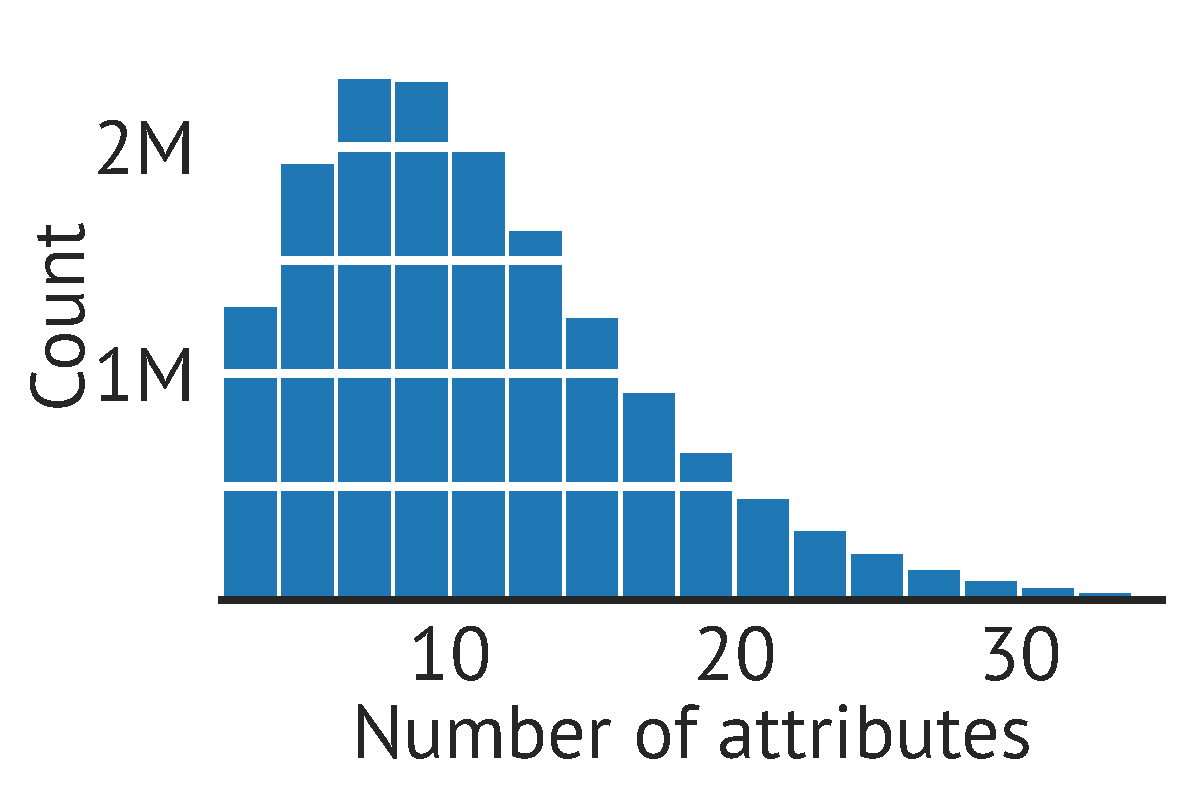
\includegraphics[width=0.6\linewidth]{ch-rfs/fig/hist_meals}
%  \vspace*{-8mm}
  \caption{A histogram of the number of foods illustrates the statistical
    challenge of building models to rank from sets. Even in this subset of the
    data, 50k users consume 16M meals in one year. This means when building a
    model to rank meals, a model with unique parameters for every datapoint is
    inefficient: models should share parameters across meals.}
  % \end{minipage}
  % \begin{minipage}[c]{0.49\linewidth}
  %   \centering
  %   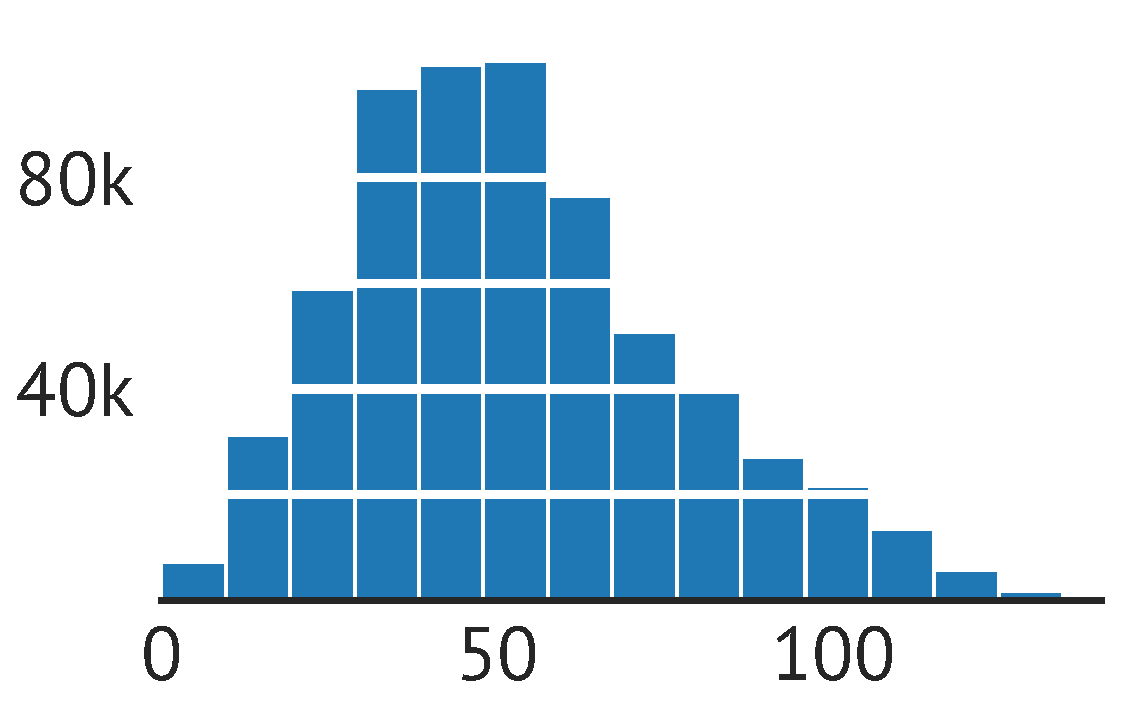
\includegraphics[width=\textwidth]{ch-rfs/fig/hist_arxiv}
  %   \vspace*{-8mm}
  %   \caption*{\# words in arXiv abstracts}
  % \end{minipage}
  % \caption{\textbf{Corpora where items have set-valued attributes have a large
  %     number of unique features.}}
  \label{fig:hist}
\end{figure}

% % hook: why you should read on. world-as-it-could-be if you join us on the ride
% We develop \gls{rfs}, a recommendation model that meets the above
% criteria of parameter-sharing and order-invariance, and guarantees improvement
% in recall and ability to approximate other models. Other order-invariant models
% such as matrix factorization do not have such theoretical backing of improved
% evaluation metrics and ability to approximate other models. The theory we
% develop for \gls{rfs} frees practitioners to focus on building
% efficient architectures for one model, rather than comparing across that may not
% be able to approximate others, or that may not provably improve recall.
% % at a high level, what are the insights needed to solve the problem?
% The key insight that guarantees that \gls{rfs} improves recall is
% the framing of recall as classification. Recall measures the fraction of items a
% user consumed in a ranking returned by a recommendation model. This is
% inherently a binary task: a model does or does not recall an item. It follows
% that a perfect classifier maximizes recall. This framing enables us build
% \gls{rfs} as a classifier and leverage recent innovations from
% deep learning~\citep{Mikolov2013} to fit our model. We define negative samples as
% items users are unlikely to consume. This allows us to fit
% \gls{rfs} to implicit feedback data, where there are only
% user-item interactions, and users do not explicitly indicate dislike of items.
% % universal approximation
% The second goal of building a model that approximates others is achieved by
% parameterizing \gls{rfs} using neural networks. This enables us to
% show that the model can approximate other recommenders that rank from sets. We
% describe several neural network architectures, including one based on residual
% networks~\citep{DBLP:journals/corr/HeZRS15}.
% % describe our model, how it is trained, an how it recommends
% \gls{rfs} is a classifier whose output is the probability of a
% user consuming an item. The model is trained to discriminate items users consume
% from items users are unlikely to consume (negative samples). The probability
% of item consumption output by the model is used to rank items for
% recommendation.
% % deep learning-> universal approximation, and architectures to satisfy
% % order-invariance and parameter-sharing
% We parameterize \gls{rfs} using neural networks, enabling the
% approximation of other models. The architectures of the neural networks are
% defined to meet the criteria of parameter-sharing and order-invariance arising
% from the properties of items represented by sets of attributes.
% % results
% We demonstrate our method by comparing it to several recommendation models on
% two datasets. The first dataset consists of users consuming $16$M meals from a
% food tracking app, and the second consists of users consuming $637$k preprints
% on the arXiv. The model outperforms order-invariant recurrent neural
% networks~\citep{Hochreiter1997}, a word embedding model~\citep{Mikolov2013}, and
% content-based Poisson factorization~\citep{Gopalana}. We also find that
% \gls{rfs} yields interpretable patterns in user behavior as in
% \Cref{fig:arxiv_tsne}.
% \paragraph{Related work.} Regression models such as deep
% sets~\citep{DBLP:journals/corr/ZaheerKRPSS17} have been developed for set-valued
% data. The deep sets model is a regression, not recommendation model, and does
% not use negative sampling in contrast to \gls{rfs}. Several
% recommendation algorithms use negative sampling to improve performance
% \citep{he2017neural,Chen:2017:SSN:3097983.3098202}. There are also deep learning
% models for collaborative filtering~\citep{zhang2017deep}. However, such work is
% centered on recommending items without side information. We focus on items with
% side information comprised of sets of attributes. In this regime the large
% number of unique sets of attributes is an obstacle and requires additional
% modeling choices. \citet{tansey2016diet2vec} also analyze diet data, but do not
% address recommendation. Probabilistic deep learning approaches for
% recommendation exist~\citep{Ranganath:2015} but do not include negative samples
% in the likelihood; we show this improves performance.
% % set up the task of recommendation, foreshadow how we will solve it via
% % classification
% Sets of attributes represent many types of items. A user might be associated
% with a photo that has tags, a disease with diagnosis codes, or a playlist of
% songs. Recommendation models for such items use the item attributes to rank
% items for users. Central to building recommendation models is evaluation, and a
% common metric is recall. But existing models such as matrix factorization do not
% have associated theoretical guarantees of improved recall. Currently, models are
% built on a case-by-case basis and adapted to the data at hand, and must be
% painstakingly compared to see which extension leads to improvement of the
% evaluation metric.
% % foreshadow desiderata
% Our goal is to build a recommendation model to rank items from attributes, and
% buttress the model with theoretical guarantees of universal approximation
% (ability to approximate other models) and of improved recommendation performance
% vis-\`a-vis recall.
% % desideratum #1: statistical challenge
% Building models that rank items from sets of attributes must address two
% difficulties arising from the properties of sets. The first difficulty is the
% statistical challenge posed by the large number of possible sets. The number of
% sets of attributes is large; we cannot posit a model with unique parameters for
% every set of attributes. The meal recommendation problem illustrates this
% statistical challenge. \Cref{fig:hist} shows the number of meals in data from a
% food tracking app. Even in this small fraction of the data, there are over ten
% million unique meals. In building a recommendation model to rank meals based on
% their constituent foods, the model should satisfy the criterion of
% parameter-sharing, and share parameters across meals with similar foods. For
% example, matrix factorization does not satisfy this criteria: it requires
% learning parameters for every meal. This is inefficient, as most meals are
% consumed by a single user in this data. The criterion of parameter-sharing is
% necessary for models to scale to large real-world datasets as in
% \Cref{fig:hist}.
% % desideratum #2
% In addition to parameter-sharing across sets, models that rank items based on
% their sets of attributes must be invariant to the order of set elements. This
% criterion is called order-invariance. For example, a meal is a set of foods, and
% remains the same meal if we permute the foods it contains. Recommendation models
% should yield the same output regardless of the order that set elements are fed
% to the model. Matrix factorization is an example of an order-invariant model.
% \begin{figure}[t!]
  \centering
  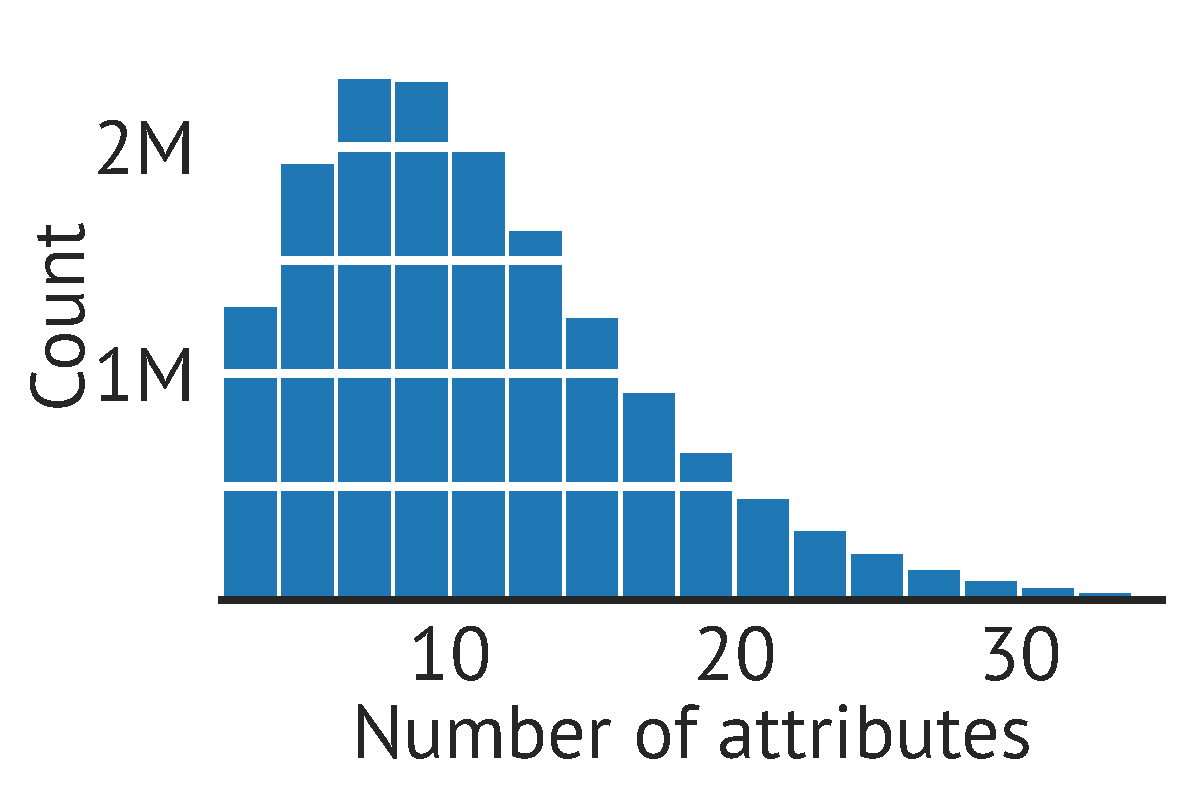
\includegraphics[width=0.6\linewidth]{ch-rfs/fig/hist_meals}
%  \vspace*{-8mm}
  \caption{A histogram of the number of foods illustrates the statistical
    challenge of building models to rank from sets. Even in this subset of the
    data, 50k users consume 16M meals in one year. This means when building a
    model to rank meals, a model with unique parameters for every datapoint is
    inefficient: models should share parameters across meals.}
  % \end{minipage}
  % \begin{minipage}[c]{0.49\linewidth}
  %   \centering
  %   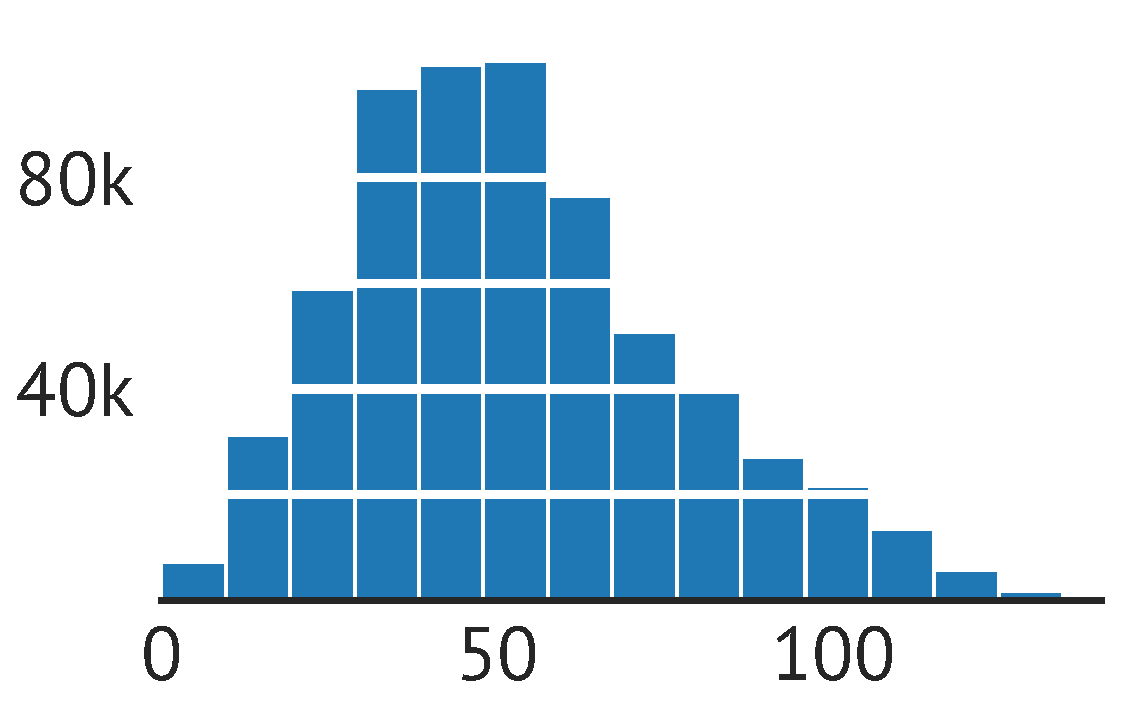
\includegraphics[width=\textwidth]{ch-rfs/fig/hist_arxiv}
  %   \vspace*{-8mm}
  %   \caption*{\# words in arXiv abstracts}
  % \end{minipage}
  % \caption{\textbf{Corpora where items have set-valued attributes have a large
  %     number of unique features.}}
  \label{fig:hist}
\end{figure}

% % hook: why you should read on. world-as-it-could-be if you join us on the ride
% We develop \gls{rfs}, a recommendation model that meets the above
% criteria of parameter-sharing and order-invariance, and guarantees improvement
% in recall and ability to approximate other models. Other order-invariant models
% such as matrix factorization do not have such theoretical backing of improved
% evaluation metrics and ability to approximate other models. The theory we
% develop for \gls{rfs} frees practitioners to focus on building
% efficient architectures for one model, rather than comparing across models that
% may not provably improve recall (or be able to approximate other models).
% % at a high level, what are the insights needed to solve the problem?
% The key insight that guarantees that \gls{rfs} improves recall is
% the framing of recall as classification. Recall measures the fraction of items a
% user consumed in a ranking returned by a recommendation model. This is
% inherently a binary task: a model does or does not recall an item. It follows
% that a perfect classifier maximizes recall. This framing enables us build
% \gls{rfs} as a classifier and leverage recent innovations from
% deep learning~\citep{Mikolov2013} to fit our model. We define negative samples as
% items users are unlikely to consume. This allows us to fit
% \gls{rfs} to implicit feedback data, where there are only
% user-item interactions, and users do not explicitly indicate dislike of items.
% % universal approximation
% The second goal of building a model that approximates others is achieved by
% parameterizing \gls{rfs} using neural networks. This enables us to
% show that the model can approximate other recommenders that rank from sets. We
% describe several neural network architectures, including one based on residual
% networks~\citep{DBLP:journals/corr/HeZRS15}.
% % describe our model, how it is trained, an how it recommends
% \gls{rfs} is a classifier whose output is the probability of a
% user consuming an item. The model is trained to discriminate items users consume
% from items users are unlikely to consume (negative samples). The probability
% of item consumption output by the model is used to rank items for
% recommendation.
% % deep learning-> universal approximation, and architectures to satisfy
% % order-invariance and parameter-sharing
% We parameterize \gls{rfs} using neural networks, enabling the
% approximation of other models. The architectures of the neural networks are
% defined to meet the criteria of parameter-sharing and order-invariance arising
% from the properties of items represented by sets of attributes.
% % results
% We demonstrate our method by comparing it to several recommendation models on
% two datasets. The first dataset consists of users consuming $16$M meals from a
% food tracking app, and the second consists of users consuming $637$k preprints
% on the arXiv. The model outperforms order-invariant recurrent neural
% networks~\citep{Hochreiter1997}, a word embedding model~\citep{Mikolov2013}, and
% content-based Poisson factorization~\citep{Gopalana}. We also find that
% \gls{rfs} yields interpretable patterns in user behavior as in
% \Cref{fig:arxiv_tsne}.
% \paragraph{Related work.} Regression models such as deep
% sets~\citep{DBLP:journals/corr/ZaheerKRPSS17} have been developed for set-valued
% data. The deep sets model is a regression, not recommendation model, and does
% not use negative sampling in contrast to \gls{rfs}. Several
% recommendation algorithms use negative sampling to improve performance
% \citep{he2017neural,Chen:2017:SSN:3097983.3098202}. There are also deep learning
% models for collaborative filtering~\citep{zhang2017deep}. However, such work is
% centered on recommending items without side information. We focus on items with
% side information comprised of sets of attributes. In this regime the large
% number of unique sets of attributes is an obstacle and requires additional
% modeling choices. \citet{tansey2016diet2vec} also analyze diet data, but do not
% address recommendation. Probabilistic deep learning approaches for
% recommendation exist~\citep{Ranganath:2015} but do not include negative samples
% in the likelihood; we show this improves performance.
% !TEX root = ../main.tex
% \section{Modeling desiderata}
% \label{sec:desiderata}
% Our goal is to build a recommendation model that provably maximizes an
% evaluation metric. The model should also approximate other models that recommend
% items based on sets of attributes. We propose criteria for models that rank from
% sets, and then exhibit a model satisfying these desiderata:
% \begin{itemize}
% \item Order-invariance: if the input to the model includes an unordered set of
%   attributes, the output of the model should not depend on the order that the
%   set elements are fed to the model.
% \item Improved recall: training the model should provably improve the evaluation
%   metric of recall. Models that satisfy this desideratum make good recommenders.
%   (In contrast, it is unclear whether a model that reconstructs the training
%   data well will lead to maximum recall performance.)
% \item Universal approximation: the model should be able to approximate any other
%   order-invariant model. This reduces the need to compare to other models in
%   lieu of comparing parameterizations of a single model.
% \item Parameter-sharing: the model should share parameters across items with
%   similar sets of attributes. This enables the model to scale to large
%   real-world datasets.
% \end{itemize}
% The criterion of order-invariance is necessary due to the set-valued features
% associated with every item. The parameter-sharing desideratum further narrows
% the set of models and guides the development of architectures parameterizing a
% model. The desiderata of improved recall and universal approximation, if
% satisfied, frees practitioners to focus on building architectures for a single
% model. Intra-model comparisons, rather than arduous inter-model comparisons,
% enable the development of generic architectures that work across many datasets
% for ranking from sets.
\section{RankFromSets}
\label{sec:rankfromsets}
\acrfull{rfs} is a class of recommendation models that recommend items with attributes to users. Let~$u~\in~\{1, \ldots, N\}$ be a user, $m \in \{1, \ldots, M\}$ be an item, and $\yum~\in~\{0,1\}$ be a binary indicator where $1$ indicates user $u$ consumed item $m$. For each item $m$, there is an associated set of attributes $x_m \in \{0,1\}^{|V|}$ from a vocabulary of $V$ attributes. The observed data is a collection of user-item interactions $\{(u, m)\}$ and the sets of attributes associated with items $\{x_m\}$.

We assume that a recommendation model is given a budget of $K$ recommendations to be made for each user. In response, the recommender system produces a list of $K$ distinct recommendations $\mathbf{r}_u~=~(r_{u1}, \ldots, r_{uK})$ for each user. The goal of the recommendation task in this paper is to maximize the expected Recall@$K$,
\begin{equation}
\textrm{Recall}@K = \mathbb{E}_{u}\left[\frac{\sum_{r \in \mathbf{r}_u} y_{ur}}{\sum_{m} \yum}\right]\, ,
\label{eq:recall}
\end{equation}
with the expectation over users in the empirical distribution $\cD$.

We combine three techniques to maximize Recall@$K$ with \gls{rfs}. First, we cast recommendation as a classification task. Second, we learn user- and attribute-level embeddings. Statistical strength is shared between items with similar attributes by representing items as the mean of their attribute embeddings. Third, we scale \gls{rfs} to large datasets using a stochastic optimization-based negative sampling training procedure.

\gls{rfs} casts the recommendation problem as a classification task. Given a user-item pair $(u,m)$ and regression function $f$, \gls{rfs} learns to predict the probability that item~$m$~will be consumed by user $u$:
$$p(\yum = 1 \mid u, m) = \sigma\left( f \left (u, x_m\right) \right)\, ,$$
where $x_m$ is the set of attributes of item $m$ and $\sigma$ is the sigmoid function. Recommendations made by \gls{rfs} are the maximum likelihood set formed by ranking a set of items for a user according to the model $f(u, x_m)$. We motivate treating recommendation as classification with the following observation.
% \begin{equation}
% \label{eqn:argmax}
% \mathbf{r}_u(K) = \underset{\mathbf{r} \in \mathbb{N}^K}{\text{argmax}} \sum_{m\in\mathbf{r}} f \left( u, x_{m} \right) \, .
% \end{equation}
% Setup the problem here as a generic classification problem. the recommendations are going to be the argmax over the probabilities output by a classifier.
% \vspace{0.5cm}
\begin{prop}
\label{prop:maximizing-recall}
Let $u \in \mathcal{U}$ be a user, $m \in \mathcal{M}$ be an item, and
$y(u,m) \in \{0,1\}$ be an indicator of whether user $u$ logged item $m$. Let
$\mathcal{E}$ be the worst-case error for binary classifier $\hat{y}(u,m)$ on
any~$(u,m)$ pair drawn from the data $\mathcal{D}$,
\begin{equation*}
  \mathcal{E} = \max_{(u, m) \in \mathcal{D}} \mathbb{1}\left[ \hat y(u, m) \neq y(u, m) \right] \, .
\end{equation*}
A binary classifier with zero worst-case error ($\mathcal{E}=0$) maximizes
recommendation recall.
\end{prop}
\begin{proof}
  A model with zero worst-case error is a perfect classifier, assigning greater probability to data with positive labels than to data with negative labels. In other words, it ranks positive examples above negative examples. Recall@$K$ is measured by the fraction of items with positive labels in a ranking returned by the model. In a classifier that achieves zero worst-case error, positively-labeled datapoints must be ranked higher than other datapoints, maximizing recall.
\end{proof}

\Cref{prop:maximizing-recall} is simple, but conceptually important. Under the assumption that a perfect classifier exists, a consistent method for learning a classifier will be a consistent method for learning a recommendation system that targets expected recall. Put another way, recall is inherently binary: a model does or does not recall an item; an item is or is not in the top $K$ recommendations in the numerator of \Cref{eq:recall}. So the best one can hope to do if recall is used to assess recommendation performance is to train a binary classifier. In practice, as with any regression method, a perfect classifier is unachievable. \Cref{prop:maximizing-recall} is a guiding principle rather than a finite-sample guarantee of maximal performance. As we show in \Cref{sec:rfs-experiments}, the classification approach of \gls{rfs} performs well in practice.

For recommending items with attributes, \Cref{prop:maximizing-recall} says that building a classifier such as \gls{rfs} is optimal if we measure recommendation performance with recall. To parameterize the \gls{rfs} classifier, a regression function $f(u, x_m)$ is needed. A straightforward parameterization is an inner product,
\begin{equation}
\label{eqn:rankfromsets}
  f\left(u, x_m\right) = \theta_u^\top\left(\frac{1}{|x_m|}\sum_{j\in x_m}
  \beta_j + g(x_m)\right) + h(x_m) \, .
\end{equation}
Each element in the inner product regression function in \Cref{eqn:rankfromsets} has an intuitive interpretation. The user embedding $\theta_u \in \mathbb{R}^d$ captures the latent preferences for user $u$. This captures the individual-level tastes of a user and is analogous to the user preference vector in classical collaborative filtering or the row embedding in matrix factorization. The attribute embedding $\beta_j \in \mathbb{R}^d$ is the latent quality conveyed through item $m$ having attribute $j$. (The set $x_m$ contains only attributes with~$x_{mj}=1$. Attributes that are not associated with item $m$ are ignored.) The item embedding function~${g(x_m)\in\mathbb{R}^d}$~represents qualities not conveyed through the set of item attributes. This term in the regression function enables collaborative filtering by capturing unobserved patterns in item consumption such as popularity. We describe how to construct this function below. The scalar item intercept function $h(x_m) \in \mathbb{R}$ makes an item more or less likely due to availability.
% !TEX root = ../../main.tex
\begin{table*}[htb!]
\centering
\resizebox{1.0\textwidth}{!}{%
\begin{tabular}{p{80mm}|p{80mm}}
  \toprule
  Query Item & Nearest Item by Cosine Similarity \\
  \midrule
  Two scoops of Raisin Bran cereal, organic Moroccan green tea, almond milk,
  light honey, tap water, large banana, large strawberries
       &
         Vita Bee bread, salted butter, fresh medium tomatoes, large fried whole
         egg, small banana\\\hline
  Iceberg lettuce, cantaloupe cubes, diced honeydew melon, cherry tomatoes, olives, dry-cooked unsalted
  hulled sunflower seed kernels, chopped hard-boiled
  egg, cucumbers, dried cranberries, fat-free ranch dressing
       &
         Green leaf lettuce, chopped sweet red bell peppers, crumbled feta cheese,
         large hard-boiled egg,
         chopped cucumber, oil-roasted salted sunflower seeds, sliced radishes, sliced strawberries, pitted Calamata olives, fat-free
         balsamic vinegar\\\hline
  Boston roast pork, mackerel, artichoke hearts, spinach, pimiento-stuffed
  Manzanilla olives, carrots, mushrooms, peppercorn ranch dressing
       &
         Broiled top round steak, tomatoes, cucumber, baby yellow squash, zucchini, black olives, extra virgin olive oil\\\hline
  Meatloaf with tomato sauce, chopped sweet red bell peppers, extra virgin olive oil, cooked asparagus spears, sweet potatoes, orange, cantaloupe cubes
       &
         Chicken breast, breadcrumbs, fresh tomatoes, shredded green leaf
         lettuce, extra virgin olive oil, spinach, chopped yellow onion, sweet
         large yellow bell peppers, whole mushrooms, chili peppers, vinaigrette
  \\\hline
  Ciabatta bun, cooked skinless chicken breast, fresh baby spinach, shredded iceberg lettuce,
  shredded mozzarella cheese, ketchup, frozen yogurt bar
             &
               Small whole wheat submarine roll, broiled round roast
               beef, roasted light turkey meat without skin, fresh medium
               tomatoes, honey smoked ham, shredded iceberg lettuce, sliced mozzarella cheese\\
         \bottomrule
\end{tabular}
}
\caption[Qualitative evaluation of \textsc{rfs} for food recommendation]{\textbf{\acrlong{rfs} trained on food consumption data provides diverse meal recommendations.} \gls{rfs} with \Cref{eqn:residual} is fit to data from a diet tracking app; items are meals and attributes are the ingredients in the meal. Meals are represented the average of their attribute embeddings, and cosine similarity between meal representations is used to find the nearest neighbors of meals (user-level information cannot be shown as this is personal diet data). \gls{rfs} reveals eating patterns: for example, the second-last query meal is a mix of meat, vegetables, and fruit, and the nearest neighbor meal is a different meat with a side of salad; the last query meal is a sandwich, and its nearest neighbor is also a sandwich with different ingredients.}% This reveals
% that \acrlong{rfs} uncovers latent patterns of consumption in the attribute
% embeddings that can be leveraged to improve recommendations.
\label{tab:nearest_meals}
\end{table*}

To define scalable item embedding and item intercept functions, note that the parameterization of the item embedding function $g(x_m)$ depends on the size of the data. If the number of items is small, $g$ can function as a lookup for unique intercepts for every item. However, if the number of items is so large that unique item intercepts lead to overfitting, a scalable parameterization of item embeddings $g$ can be defined using additional information about every item. For example, if the data consists of foods in meals, we can define a meal intercept as the mean of food intercepts, yielding a scalable item intercept function. The item intercept function $h(x_m)$ that maps item attributes to scalars is constructed in the same way. We study both of these choices in \Cref{sec:rfs-experiments}.

The inner product regression function in \Cref{eqn:rankfromsets} has several benefits. It requires computing a sum over only the attributes with which each item is associated. This enables \gls{rfs} to scale to large attribute vocabularies where traditional matrix factorization methods are intractable. Second, the embed-and-average approach to set modeling is provably flexible as we show later. We now describe deep variants of \gls{rfs} and detail how \gls{rfs} can approximate other recommendation models.% Consider the example from \Cref{sec:rfs-introduction}
% of predicting whether a user
% would enjoy a meal. Each user has some preferences about which meals they enjoy.
% A meal is made up of foods or attributes. One does not need to consider foods
% that are not in a meal; unused foods can be ignored. In addition, a meal is more
% than its foods. For instance, a user trying to eat healthier may enjoy all the
% ingredients in a meal, but if it is deep fried, it will be unappealing. The
% regression function in \gls{rfs} should be able to learn such latent patterns in
% meal consumption. Finally, even if a meal is not very appealing to a user, it
% may be popular and available everywhere, making it more likely to be consumed.

% The regression function $f(u, x_m)$ parameterizes the generative process of the
% labels conditional on the item attributes and user,
% $\yum \sim \textrm{Bernoulli}\left(\yum; \sigma(f(u, x_m)\right)$.

% Specifically, recent results in deep learning for set-valued data show that
% such an approach is sufficient to model nearly any function
% \citep{DBLP:journals/corr/ZaheerKRPSS17}. In theory, it may be necessary to
% apply a nonlinearity, such as a deep neural network, to $f$ to learn any
% function. In preliminary experiments, we found increasing the embedding size
% $d$ in the embedding model offered a better tradeoff between parameter size
% and model performance than the additional parameters added by a neural
% network.

The \gls{rfs} inner product regression function in \Cref{eqn:rankfromsets} is a log-bilinear model. But there are several other choices of regression function, and we draw on the deep learning toolkit for classification to build two other example architectures. With finite data and finite compute, one architecture may outperform another, or prove insufficient to capture patterns in user consumption. (Later, we show that all architectures are equivalent under fewer assumptions.) First, as an alternative to the log-bilinear model in \Cref{eqn:rankfromsets}, we can use a deep neural network as a regression function:
\begin{align}
  f\left(u, x_m\right) = \phi\left(\theta_u, \frac{1}{|x_m|}\sum_{j\in x_m}
  \beta_j, g(x_m)\right) + h(x_m) \, ,
  \label{eqn:neural-network}
\end{align}
where the deep network $\phi$ has weights and biases and takes as inputs the user embedding, sum of attribute embeddings, and item intercept. Such a neural network can represent functions that may or may not include the inner product in \Cref{eqn:rankfromsets}; \emph{ex~ante}, it is unclear whether a finite-depth, finite-width neural network can represent the inner product.

Another regression function for \gls{rfs} is a combination of
\Cref{eqn:rankfromsets,eqn:neural-network}, using an idea borrowed from deep
residual networks for image classification~\citep{he2015deep}. In this
architecture, a neural network $\phi$ with the same inputs as in
\Cref{eqn:neural-network} learns the residual of the inner product model:
\begin{align}
  f\left(u, x_m\right) = \theta_u^\top\left(\frac{1}{|x_m|}\sum_{j\in x_m}
  \beta_j + g(x_m)\right) + \phi + h(x_m) \, .
  \label{eqn:residual}
\end{align}
The choice of regression function in \acrshort{rfs} depends on the data. On finite data, with finite compute, one parameterization of \gls{rfs} will outperform another. To demonstrate this, we simulated synthetic data from the same generative process \gls{rfs} employs with a ground-truth regression function (a square kernel), and found that the residual and deep parameterizations outperformed the inner product architecture. These results are included in \Cref{sec:simulation}, and motivate exploring other architectures than the three examples here.
% We conclude this section by showing that in the regime of infinite
% data and compute, all the \gls{rfs} architectures we propose, including the
% inner product, can approximate other recommendation models that operate on
% set-valued input such as matrix factorization.

Stepping back from the setting of finite data and compute, a bigger picture emerges, which reveals the choice of regression function in \gls{rfs} does not matter. We show that any \gls{rfs} architecture is sufficiently flexible to approximate recommendation models that operate on set-valued input. We define permutation-invariant models before deriving this result.

The regression function $f$ in \gls{rfs} operates on set-valued input: the unordered collection of item attributes $x_m$. A set is, by definition, permutation-invariant: it remains the same if we permute its elements. Functions that operate on set-valued inputs must also be permutation-invariant. \gls{rfs} is permutation-invariant; the set of attributes associated with an item enter into \Cref{eqn:rankfromsets,eqn:neural-network,eqn:residual} via summation. Other examples of permutation-invariant recommendation models are multiple matrix factorization, models based on word embeddings, and permutation-marginalized recurrent neural networks. These models are shown to be permutation-invariant in \Cref{sec:models} and evaluated in \Cref{sec:rfs-experiments}. We now show that \gls{rfs} can approximate other permutation-invariant recommendation models such as matrix factorization.

\begin{prop}
  Assume the vocabulary of attributes (set elements) is countable, $\lvert V \rvert < \lvert \bbN_0 \rvert$. Then \acrshort{rfs} can approximate any permutation-invariant recommendation model.
  \label{prop:universal-approximation}
\end{prop}
The proof follows directly from Theorem~2 in \citet{zaheer2017deep} and we will not
restate it here. (The only change to the proof is the mapping from set elements
to one-hot vectors, $c \colon V \to \left\{0, 1\right\}^{\lvert V \rvert}$ to
yield a unique representation of every object in the powerset.)
\Cref{prop:universal-approximation} means that any of the parameterizations in
\Cref{eqn:rankfromsets,eqn:neural-network,eqn:residual} is flexible enough to
approximate other principled recommendation models that leverage item
attributes, such as multiple matrix
factorization~\citep{gopalan2014content-based,wang2011collaborative}.% This proposition also supports
% exploring other parameterizations of \gls{rfs} that may have better
% computational or statistical properties.

The parameters for \gls{rfs} are learned by stochastic optimization. Denote
the full set of \gls{rfs} model parameters by $\mbgamma$, and let~$\cD_u$~be the
empirical data distribution for a user. Let $\lambda_u$ be a reweighting
parameter. The per-user maximum likelihood objective for \gls{rfs} is
\begin{equation}
  \label{eq:objective}
  \begin{aligned}
  \cL(\mbgamma, \lambda_u) = \E_u\big[ \E_{m \sim \cD_u \mid \yum = 1}%&
  \left
  [\log p(\yum =1 \mid x_m; \mbgamma)\right]
  + \lambda_u \E_{k \sim \cD_u \mid \yuk = 0}%&
  \left[\log p(\yuk = 0 \mid x_k;
  \mbgamma)\right]
                \big]
  \end{aligned}
\end{equation}

In traditional regression, altering the ratio of positive to negative examples
by reweighting leads to inconsistent parameter estimation. The inconsistency
stems from the randomness in the labels, given the features. However, Recall@$K$ assumes that each user, item attribute set pair ($u, x_m$) uniquely determines
whether the item was consumed or not (the label $\yum$). Here, all reweightings
produce the same result. This means that for any negative example weight
$\lambda_u$, the learned model will be the same. In practice we set $\lambda_u$
to balance the positive and negative examples for each user. We use stochastic
optimization to maximize \Cref{eq:objective}, and describe two negative sampling
schemes that are dependent on the choice of evaluation metric.
% for a single datapoint $(x_m, \yum=1)$ is
% \begin{align}
% \begin{split}
%   \cL(\theta, & (x_m, \yum), \{(x_k, \yuk)\}) =\\
%   &\log p(\yum = 1 \mid x_m; \theta) + \sum_{k=1}^L \log p(\yuk = 0 \mid x_k;
%   \theta),\\
%   &\textrm{with}~x_k\sim\textrm{Uniform}(I).
%   \label{eq:objective}
% \end{split}
% \end{align}
% As users only interact with a small number of items, this objective function is
% dominated by negatively-labeled datapoints with~$\yum = 0$. We use stochastic
% optimization to maximize \Cref{eq:objective} and learn parameters jointly.
% Stochastic optimization requires subsampling the terms in the objective with
% negative labels. Such subsampling directly leads to a binary classification
% binary classification loss function with negative samples, as in previous work
% on word embeddings~\citep{mikolov2013distributed} and recommender
% systems~\citep{he2017neural,song2018neural}.
% The \gls{rfs} parameterization in
% \Cref{eqn:prob_y_given_um,eqn:argmax,eqn:rankfromsets} is bi-convex and could be
% fit through alternating coordinate descent. That is, fixing the user embeddings,
% the problem is convex in each of the other parameters; similarly, the problem is
% convex in the user parameters if the other parameters are fixed. For each
% coordinate in the user step, such a procedure would require iterating over all
% items. The massive number of items in the datasets in \Cref{sec:rfs-experiments}
% makes this intractable; similar issues could also arise for datasets with many
% users.
% \paragraph{Negative sampling} All observed positive labels (i.e. instances where
% $\yum = 1$) are divided into mini-batches. For each mini-batch, each
% positively-labeled sample is paired with a negatively-labeled sample. The
% negatively-labeled sample has the same user as its paired sample, but the item
% is sampled uniformly from a set of items. This procedure is not unbiased, but
% still leads to a consistent classifier: note that any reweighting of items that
% assigns nonzero weight to all items can be arbitrarily biased, but still lead to
% a consistent classifier. As long as every item has nonzero weight, the infinite
% data limit ensures that the classifier will learn to discriminate between
% positively- and negatively-labeled datapoints. We decide to balance
% positively-labeled datapoints with negative samples in each mini-batch as it is
% easy to implement as shown in \Cref{sec:code}.
% We note that any negative sampling
% scheme that assigns nonzero weight to every item leads to a consistent
% classifier.

% Ideally, the sampling set should be the set of all items which the user has not
% consumed, where~$\yum~=~0$. But maintaining and sampling from user-specific sets
% of negative labels can be computationally prohibitive. When the item set is
% large and labels are sparse (that is, $\yum = 0$ for most user, item pairs),
% embedding models are often trained by drawing negative samples uniformly from
% the item set~\citep{mikolov2013distributed}. For training \gls{rfs}, we propose
% two different negative sampling distributions that trade off quality of the
% learned parameters for scalability of the training procedure.

Negative samples can be drawn uniformly over the entire corpus of items, which we define to be corpus sampling. If the item set is large, this can be an expensive procedure. This negative sampling scheme leads to objective functions used in other recommender systems~\citep{he2017neural,song2018neural}.

On large datasets, it is infeasible to calculate Recall@$K$ for evaluation, as this requires ranking every item for every user (e.g. in \Cref{sec:rfs-experiments} we study a dataset with over $10$M items). We define a scalable evaluation metric based on recall, and describe how it leads to a natural choice of negative sampling distribution.

Sampled recall is defined as follows. Consider held-out datapoints with positive labels,~${(x_m, \yum = 1)}$. For every held-out datapoint, $K-1$ datapoints with negative labels~${(x_k, \yuk = 0)}$ are sampled from the rest of the held-out data, which together yield a set of $K$ datapoints. A recommendation model is used to rank the $K$ datapoints $r_{u1}, \ldots, r_{uK}$. SampledRecall@$k$ is the fraction of the $K$ held-out datapoints that the model ranks in the top~$k$:
\begin{equation}
  \textrm{SampledRecall@}k = \frac{1}{K}{\E_{um}\left[\sum_{r\in
\{\mb{r}_{u1},
\ldots \mb{r}_{uk}\}} y_{ur}\right]}\, .
\label{eq:sampled-recall}
\end{equation}

The expectation is over users and items in the held-out set of datapoints. This evaluation metric is scalable: instead of using a model to rank every item, SampledRecall@$k$ requires ranking only $K$ items. Sampled recall is~$1$~if $k~=~K$, as the held-out datapoint with $\yum = 1$ is in each list of $K$ datapoints to be ranked. This metric is used in recommender systems when the number of items is large~\citep{ebesu2018collaborative,yang2018openrec:}.
% For
% example, with $M=10$, an average sampled recall@1 of $0.5$ means for 50\% of the
% held-out datapoints, the item consumed by the user was ranked first by the model
% (out of $9$~items randomly sampled from the held-out data of other users). For
% the sampled recall metric we choose $M=10$, meaning $9$ `fake' meals are sampled
% uniformly from other users' meals in the held-out validation and test sets.

When sampled recall is used as an evaluation metric, batch sampling is a natural way to draw negative samples. Sampled recall is calculated on items drawn from other user's data. We define batch sampling as generating negative samples by permuting mini-batch items. Besides corresponding to the sampled recall metric, this technique is memory-efficient, as it requires that only the current mini-batch be in memory.

In addition to scalability, both negative sampling procedures above have
the advantage of implicitly balancing the classifier. As shown in
\citet{veitch2019empirical}, using stochastic gradient descent with
negative sampling is equivalent to a Monte Carlo approximation of the
reweighted (balanced) classification loss.

% !TEX root = ../main.tex
\section{Permutation-invariant Recommender Models}
\label{sec:models}
\Cref{prop:universal-approximation} shows that \gls{rfs} can approximate permutation-invariant recommendation models. We describe several common recommendation models and show that they are permutation-invariant, before comparing their performance to \gls{rfs} in \Cref{sec:rfs-experiments}.

\citet{gopalan2014content-based} develop a probabilistic matrix factorization model of user consumption data. \Gls{ctpf} models user preferences using a generative process,
% !TEX root = ../main.tex
\begin{enumerate}
  \item \textbf{Document model:}
  \begin{enumerate}
  \item Draw topics $\beta_{vk} \sim \Gam(a, b)$
  \item Draw document topic intensities $\theta_{dk} \sim \Gam(c, d)$
  \item Draw word count $w_{dv} \sim \Pois(\theta_d^T \beta_v)$.
  \end{enumerate}
  \item \textbf{Recommendation model:}
  \begin{enumerate}
  \item Draw user preferences $\eta_{uk} \sim \Gam(e, f)$
  \item Draw document topic offsets $\epsilon_{dk} \sim \Gam(g, h)$
  \item Draw $r_{ud} \sim \Pois(\eta_u^T (\theta_d + \epsilon_d))$.
  \end{enumerate}
\end{enumerate}
To show that \gls{ctpf} is permutation-invariant, consider the Poisson likelihood function over words $w_{dv}$. Conditional on the latent item representation $\theta_d$ and latent word representation $\beta_v$, every word in the document $w_{dv}$ is independent; the joint probability of words in a document factorizes:
\begin{align}
  p(w_{d} \mid \theta_d, \beta_v) &= \prod_{w_{dv} \in w_d} p(w_{dv} \mid \theta_d, \beta_v)\, .
\end{align}
\gls{ctpf} makes predictions using expectations under the posterior. The posterior is proportional to the the log joint of the model, and the attributes of items (words in documents) enter into the model only via the above product. The product of the probability of words in a document is invariant to a reordering of the words in the document, and therefore \gls{ctpf} is permutation-invariant.

Word embedding models~\citep{mikolov2013distributed} can be used as recommendation models if the embeddings are learned using a modified context window. For an item with attributes $x_m$, let the context window for attribute ${j\in x_m}$ be the set of other attributes of the same item ${j' \in x_m: j'\neq j}$. To recommend items using this model of attributes $\beta_j$ for $j \in V$, item embeddings are computed as the average of their attribute embeddings. Users are represented as the average of the embeddings of the items they consume, and recommendation is performed using the cosine similarity of user and item embeddings. This is a permutation-invariant model, as the output of the model depends on the sum of attribute embeddings (summation is invariant to permutation).

StarSpace is also an embedding model and represents users as a sum over a user's consumed items' attribute embeddings (there is no explicit user embedding). In contrast to the word embedding model, StarSpace is trained on a classification objective with negative samples drawn from the the set of items~\citep{wu2018starspace:}. As model predictions depend on sums of attributes, StarSpace is a permutation-invariant recommendation model.

We next consider LightFM~\citep{kula2015metadata}, a permutation-invariant recommendation model. We show that if the \gls{bpr} objective~\citep{rendle2009bpr:} is used, LightFM is an instance of \acrshort{rfs}. \footnote{The LightFM paper~\citep{kula2015metadata} uses a logistic objective to which \Cref{prop:maximizing-recall} applies. LightFM with the \gls{bpr} objective is unpublished but implemented in code released by the author. For completeness, we studied LightFM with both objectives to ensure its performance is equivalent to \gls{rfs} when the \gls{bpr} objective is used.} Although the \gls{bpr} objective is designed for ranking, models trained with it can be used to construct classifiers. The \gls{bpr} objective is
$${\log\sigma\left(f(u, x_m; \mbgamma) - f(u, x_k; \mbgamma)\right)}\, ,$$
where $m$ corresponds to a positive label $\yum = 1$, $k$ corresponds to a negative label $\yuk = 0$, and $f$ is parameterized as in \gls{rfs}~\citep{kula2015metadata}. A ranking function $f$ optimizes the \gls{bpr} objective if~${f\rightarrow \infty}$ for the positive example and $f$ is constant for the negative example; or, if $f$ is constant for the positive example and $f\rightarrow -\infty$ for the negative example. In either case, a constant can be added to yield a perfect classifier from the ranking function $f$ (positive examples are ranked higher than negative examples in the optimal ranking, so there exists such a constant). That we can construct a classifier from the \gls{bpr} objective means that \Cref{prop:maximizing-recall} applies: permutation-invariant models such as LightFM, trained with the \gls{bpr} objective, are instances of the \gls{rfs} class of recommendation models.

The regression function $f$ in \gls{rfs} can also be parameterized using a recurrent network, as in \citet{bansal2016ask-the-gru:}. Such a recommendation model can be made permutation-invariant if averaged over permutations of attributes fed to the network. Attributes are treated as a sequence and the marginalization is over these permutations,
\begin{equation}
p(\yum = 1 \mid x_m) =
  \frac{1}{\lvert \pi(x_m) \rvert}\sum_{\pi \in \pi(x_m)}\sigma\left(\phi(\theta_u,\{\beta_{\pi(1)}, \ldots,
  \beta_{\pi(J)}\})\right) \, .
\label{eq:rnn}
\end{equation}
Here $\beta_j$ are attribute embeddings, $\pi(x_m)$ denotes the set of all permutations of the attributes $x_m$, and $\phi$ is the output of a recurrent neural network architecture~\citep{bansal2016ask-the-gru:} projected to a scalar.
% !TEX root = ../main.tex
\section{Empirical Study}
\label{sec:rfs-experiments}
We study \gls{rfs} on two datasets and tasks. The first data consists of researcher reading behavior from the arXiv; the semi-synthetic task is to recommend documents to scientists. The second is crowdsourced food consumption data from a diet tracking app, and the task is meal recommendation. On both benchmarks, models in the \gls{rfs} class outperform several baseline methods. The permutation-invariant models we compare to are described in \Cref{sec:models}, and the hyperparameters used are described in \Cref{sec:appendix-empirical}. To show the relative ease of implementation of \gls{rfs} we give example code in \Cref{sec:code}.\footnote{Full source code is available at \url{https://github.com/altosaar/rankfromsets} for reproducibility.}

\paragraph{Recommending Research Papers.} We benchmark \gls{rfs} on data of scientists reading research papers on the arXiv, where the goal is to recommend papers to scientists. This is a semi-synthetic task: it uses real-world data, but the item side information (article abstracts) is not set-valued. Nevertheless, document recommendation is a standard benchmark to study whether \gls{rfs} performs well in settings outside its target purview of meal recommendation. The arXiv data represents one year of usage (2012) and consists of $65$k users, $636$k preprints, and $7.6$M clicks. For evaluation, we match \citep{gopalan2014content-based}, using the same test and validation splits and the same set of held-out $10$k users. As in~ \citep{gopalan2014content-based} we compute precision in addition to recall. The held-out validation and test splits each consist of $20\%$ of the clicks and $1\%$ of the documents. In-matrix documents refer to documents that have clicks in the training data, while out-matrix or cold-start documents have no previous clicks.
% !TEX root = ../../main.tex
%   \hspace{1.8cm}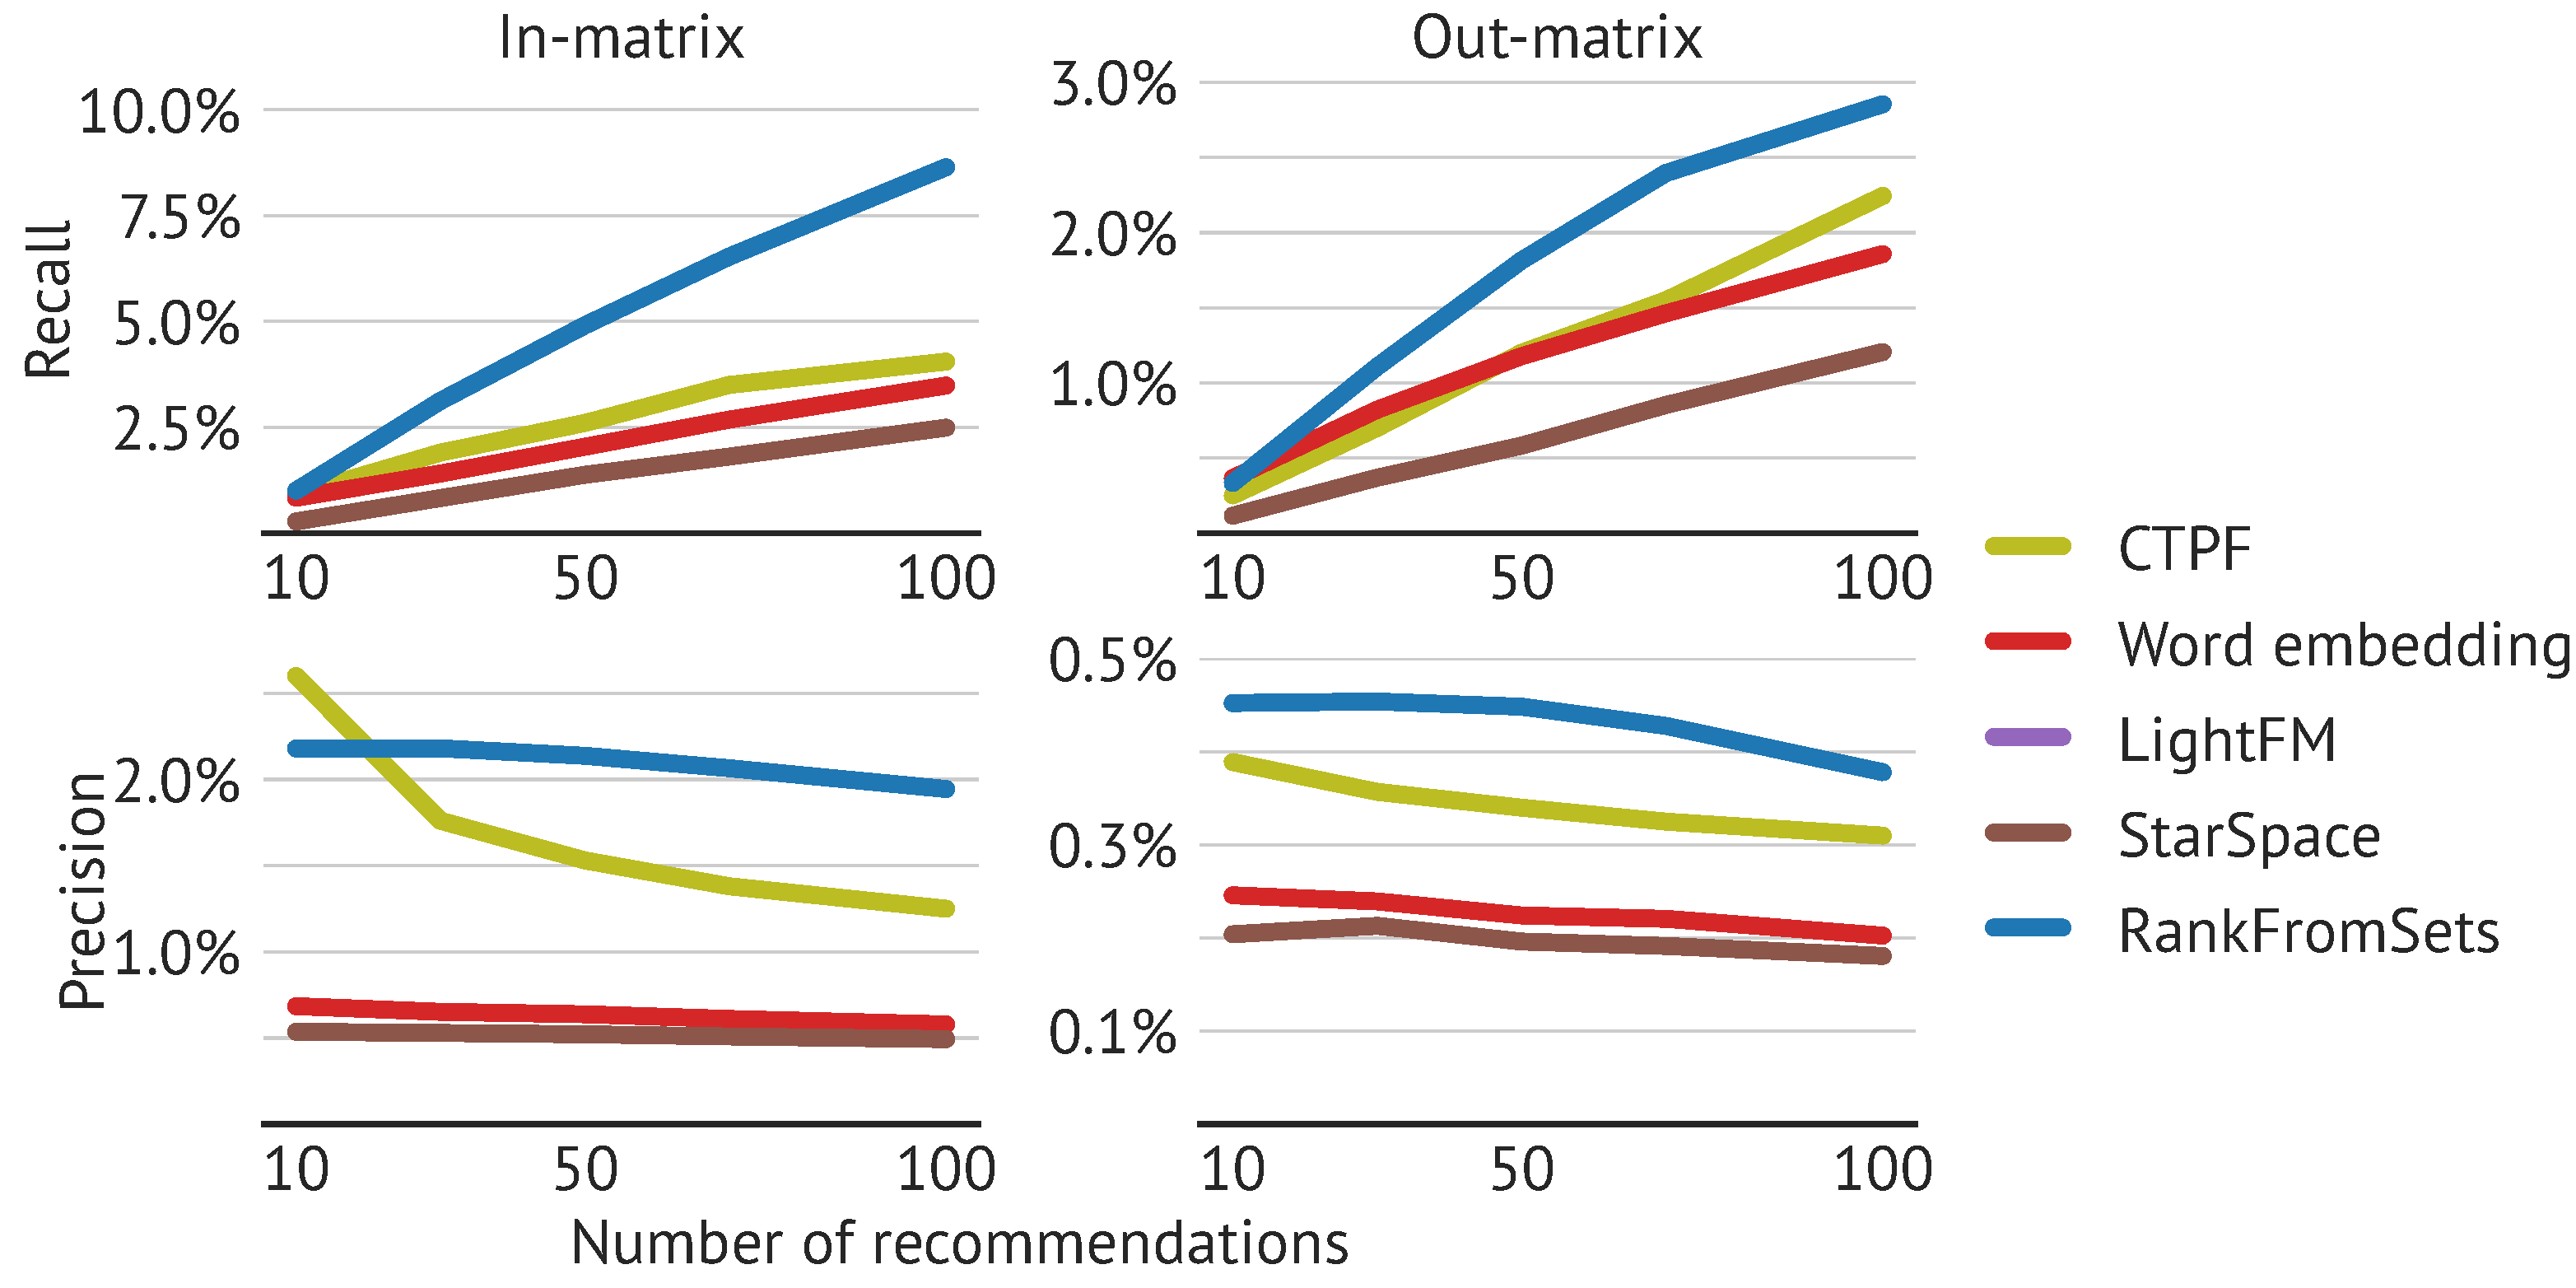
\includegraphics[width=0.7\linewidth]{ch-rfs/fig/arxiv}
\begin{figure*}[t]
  \centering
  \begin{subfigure}{\linewidth}
    \centering
    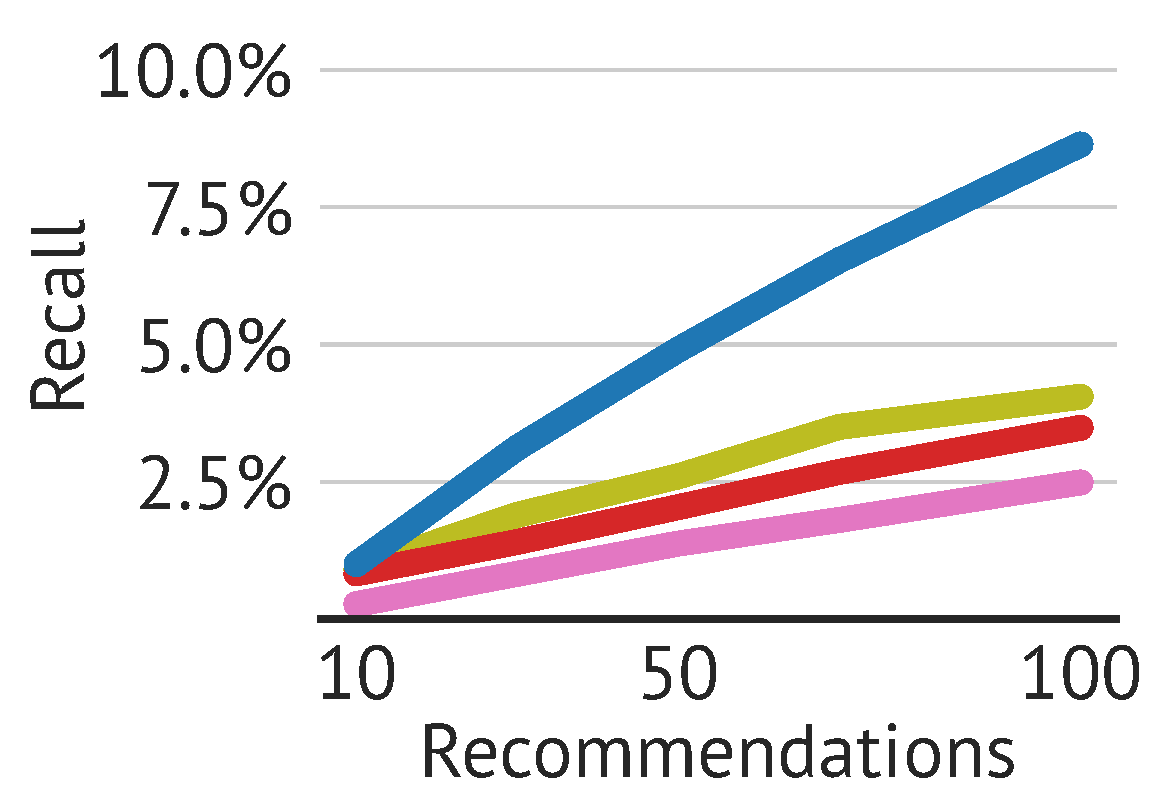
\includegraphics[width=.3\linewidth]{ch-rfs/fig/arxiv-in-matrix-recall}
    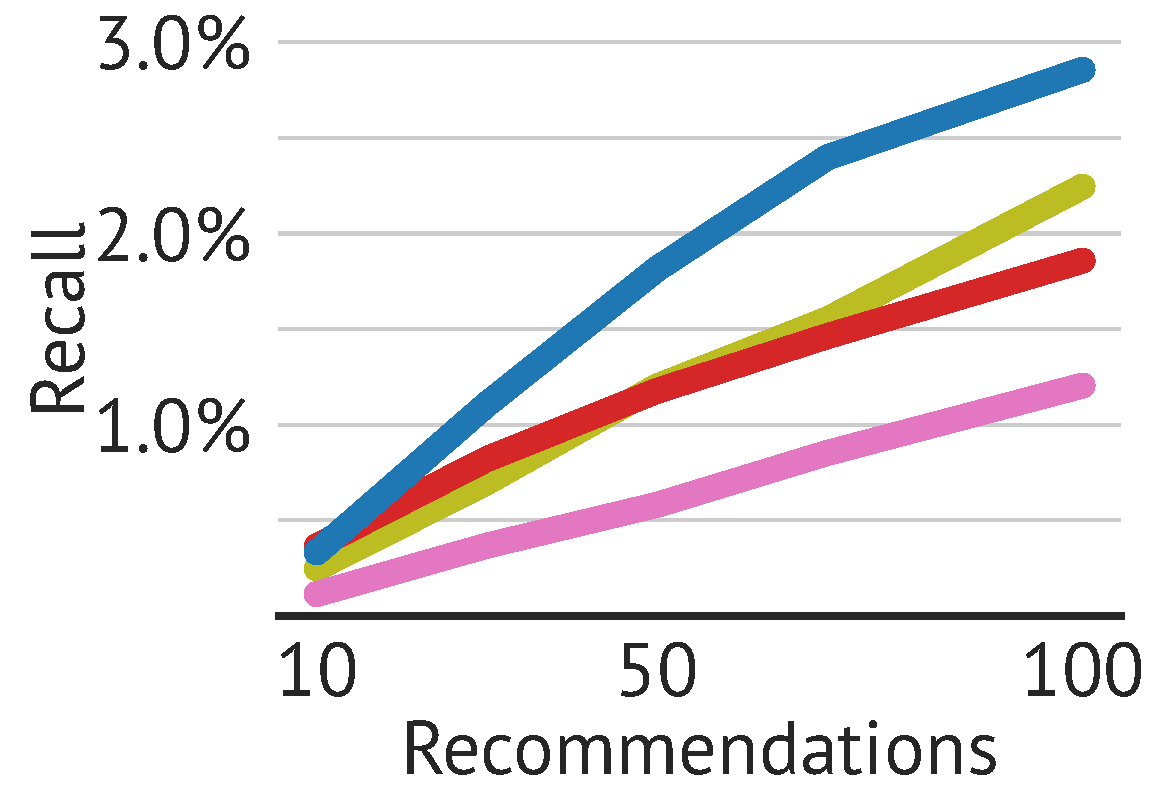
\includegraphics[width=.3\linewidth]{ch-rfs/fig/arxiv-out-matrix-recall}
    \hspace{3mm}
    \raisebox{9mm}{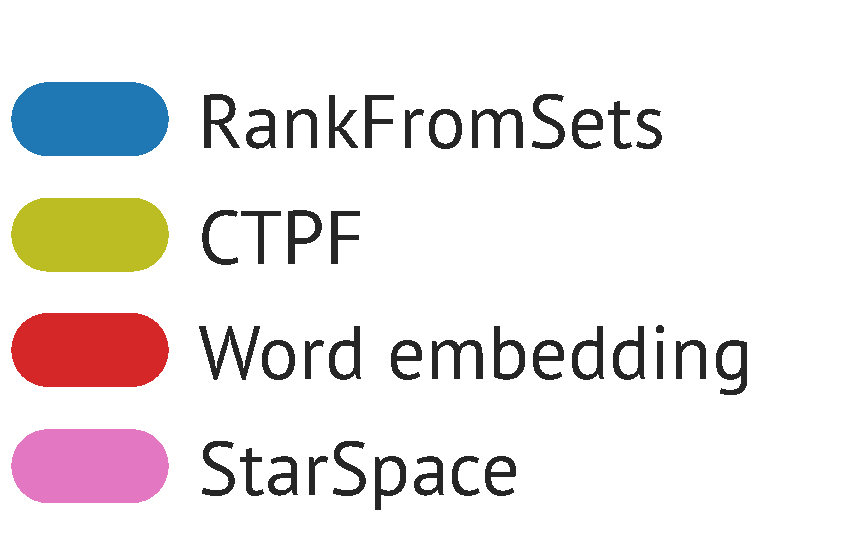
\includegraphics[width=0.2\linewidth]{ch-rfs/fig/arxiv-legend}}
    \caption{Recall for in-matrix (left) and out-matrix (right) documents.}
    \vspace*{0.5cm}
  \end{subfigure}
  \begin{subfigure}{\linewidth}
    \centering
    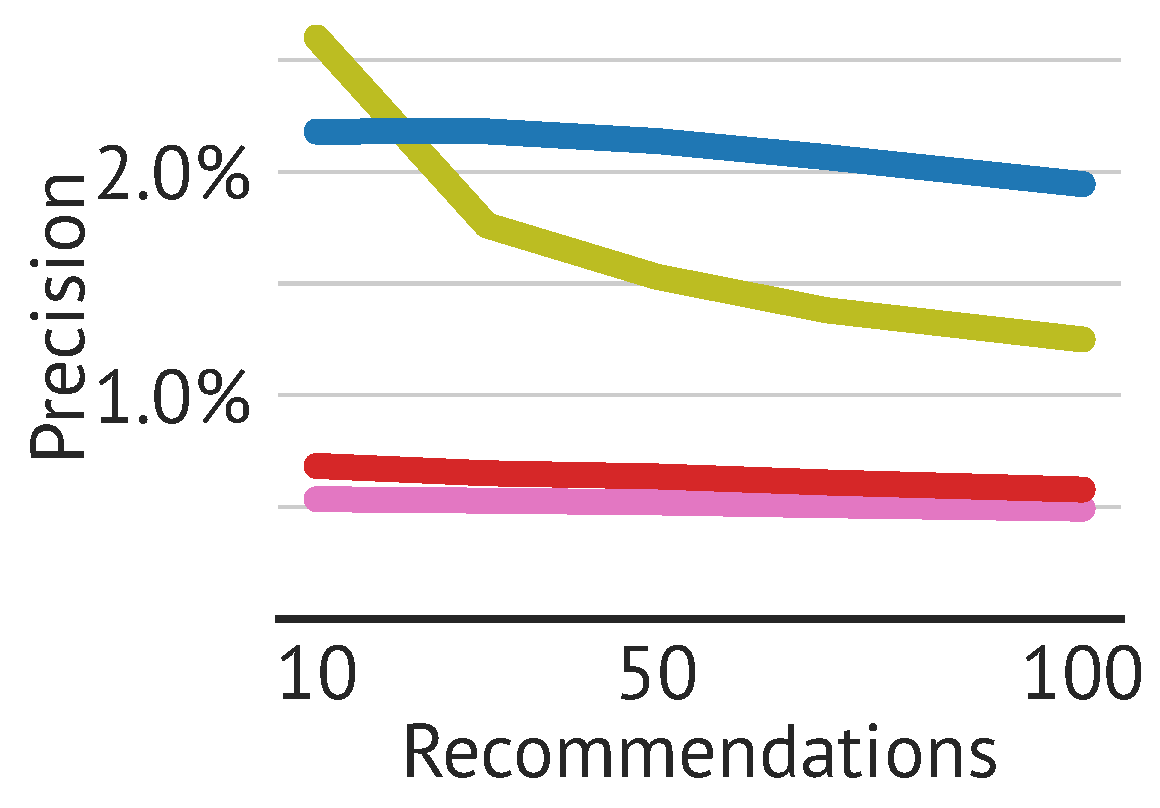
\includegraphics[width=.3\linewidth]{ch-rfs/fig/arxiv-in-matrix-precision}
    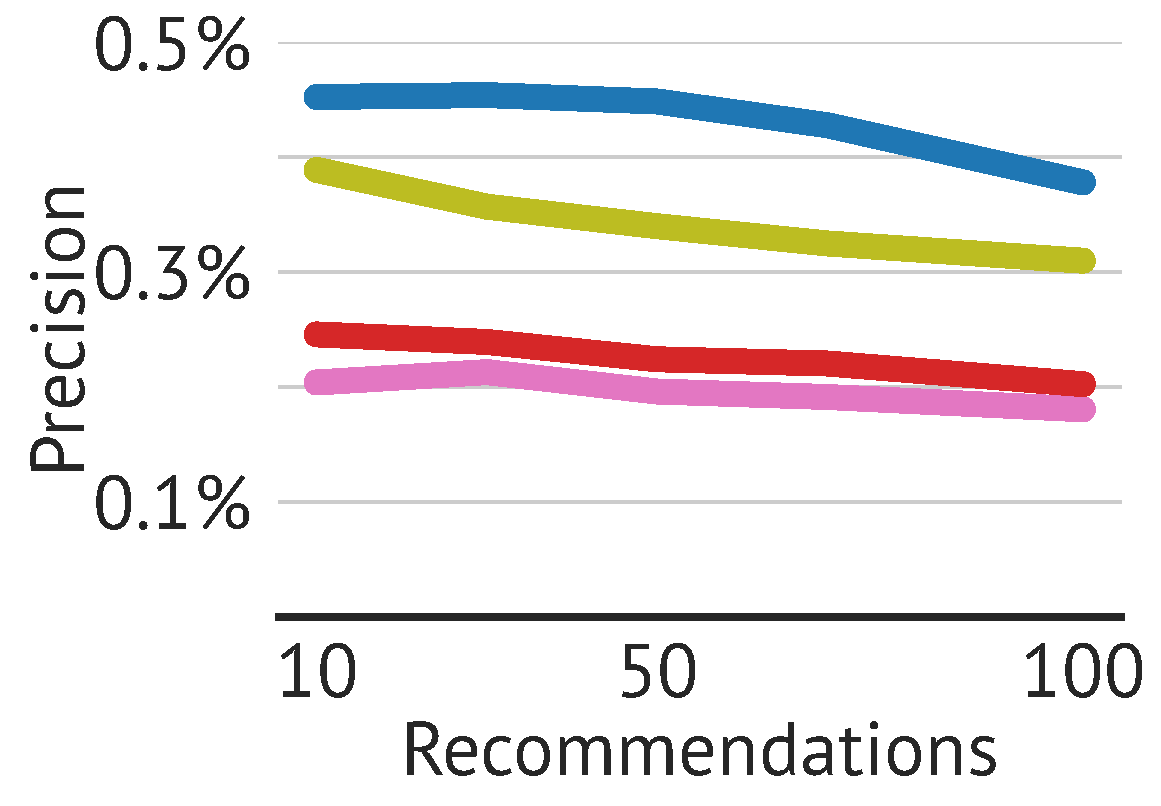
\includegraphics[width=.3\linewidth]{ch-rfs/fig/arxiv-out-matrix-precision}
    \hspace{3mm}
    \raisebox{9mm}{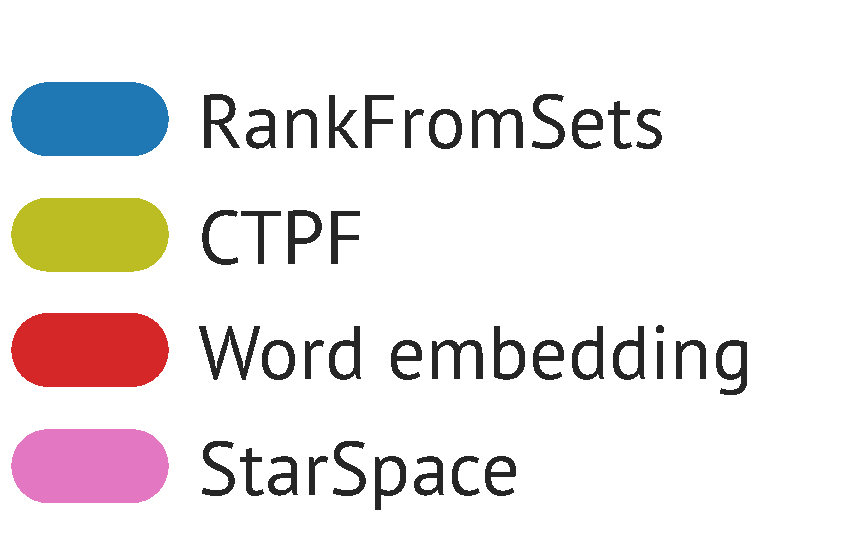
\includegraphics[width=0.2\linewidth]{ch-rfs/fig/arxiv-legend}}
    \caption{Precision for in-matrix (left) and out-matrix (right) documents.}
  \end{subfigure}
  % \begin{subfigure}[b]{\figwidthrfs}
  %   \centering
  %   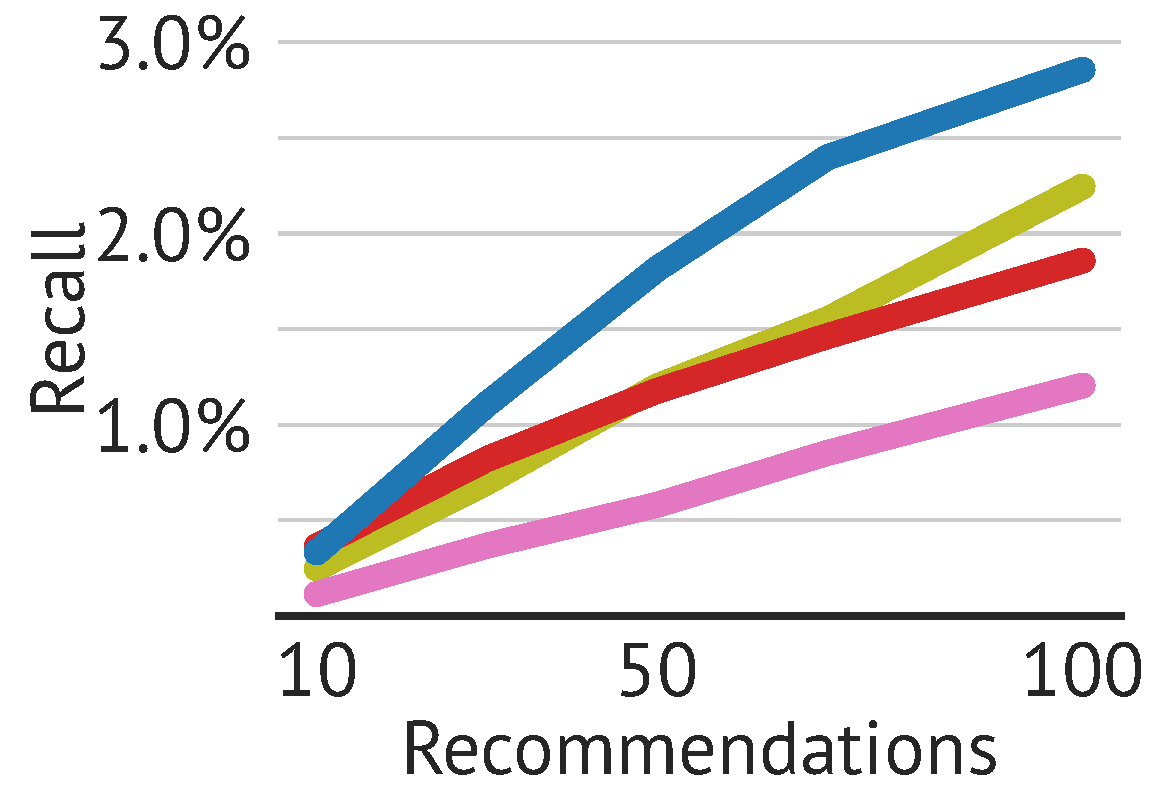
\includegraphics[width=\mysizerfs]{ch-rfs/fig/arxiv-out-matrix-recall}
  %   \caption{Out-matrix}%
  %   \label{fig:arxiv-out-recall}%
  % \end{subfigure}
  % \begin{subfigure}[b]{\figwidthrfs}
  %   \centering
  %   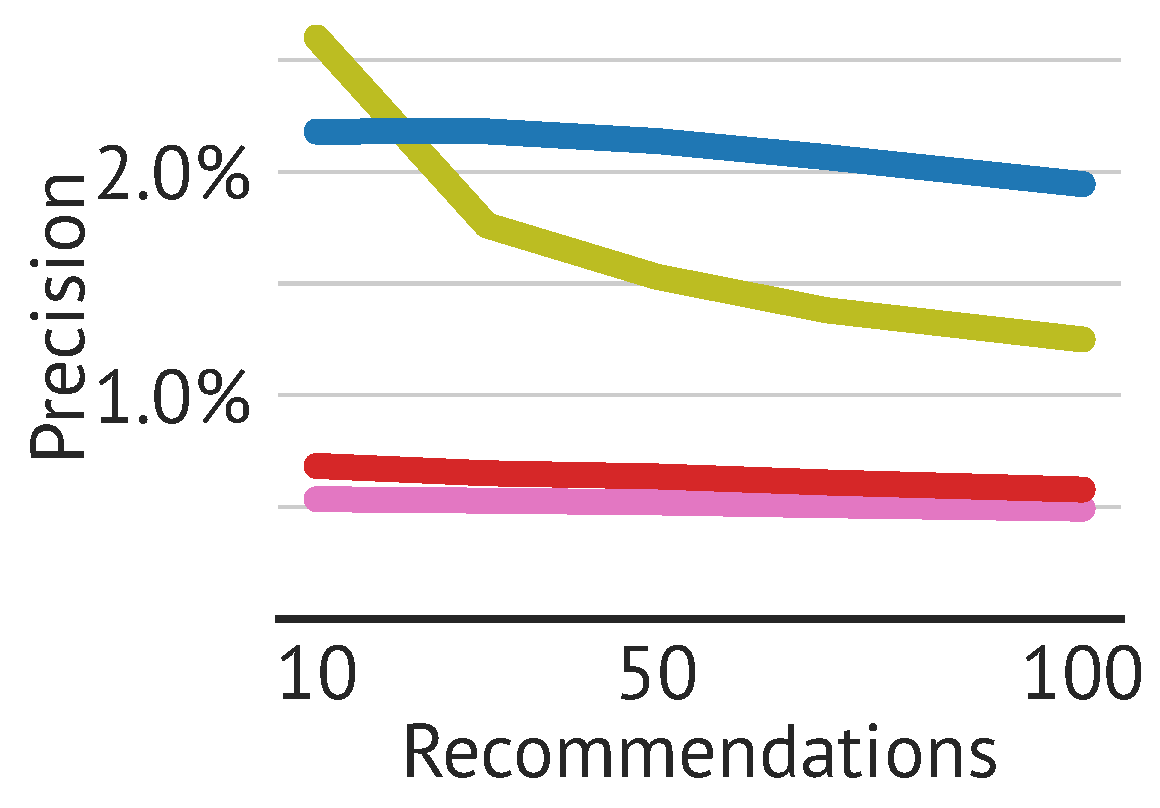
\includegraphics[width=\mysizerfs]{ch-rfs/fig/arxiv-in-matrix-precision}
  %   \caption{In-matrix}%
  %   \label{fig:arxiv-in-precision}%
  % \end{subfigure}
  % \begin{subfigure}[b]{\figwidthrfs}
  %   \centering
  %   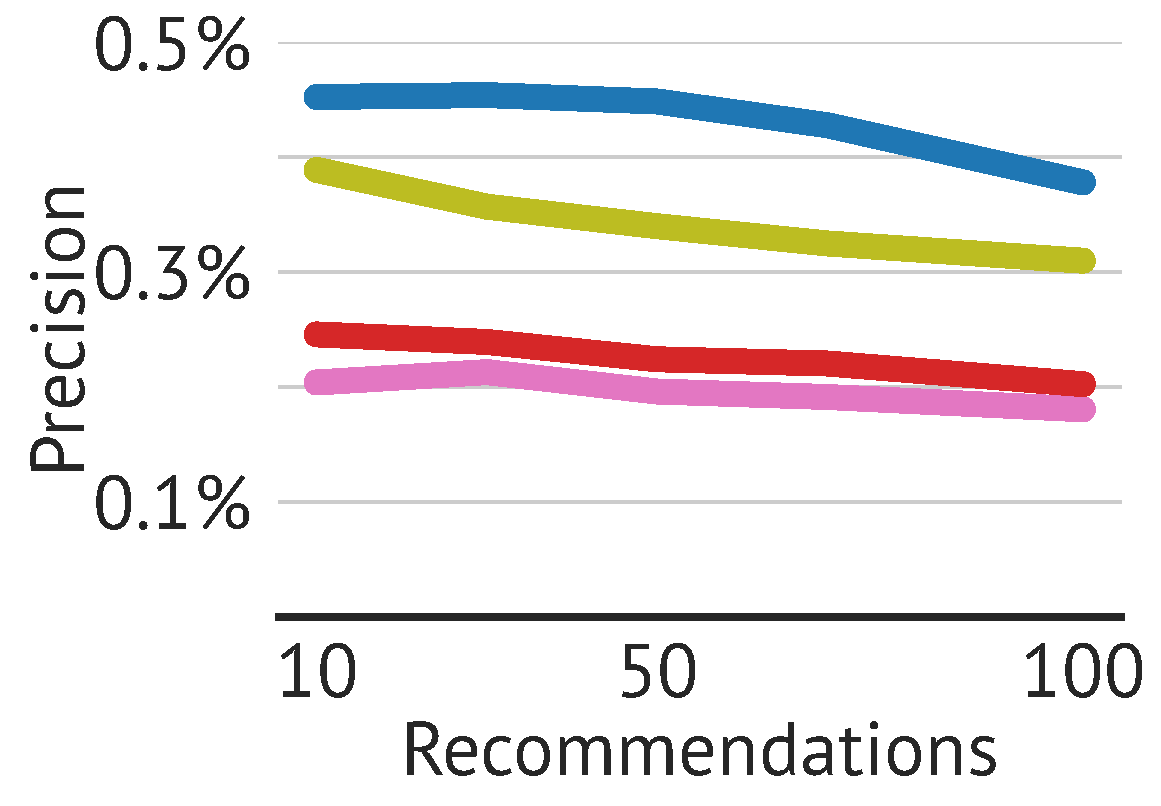
\includegraphics[width=\mysizerfs]{ch-rfs/fig/arxiv-out-matrix-precision}
  %   \caption{Out-matrix}%
  %   \label{fig:arxiv-out-precision}%
  % \end{subfigure}
  \caption[\textsc{rfs} results on arXiv data for article recommendation]{\label{fig:arxiv-performance} \textbf{\acrlong{rfs} outperforms collaborative topic Poisson factorization (\acrshort{ctpf})~\citep{gopalan2014content-based} and other models on recommending arXiv papers to scientists.} The items are documents and the attributes are the unique words in the abstracts. Recommendation performance is evaluated using both precision and recall to match the evaluation in \citep{gopalan2014content-based}. The metrics are reported on training (in-matrix) documents and cold-start (out-matrix) documents with no clicks in the training set. All \acrshort{gru} and \acrshort{lstm}-based models in \citet{bansal2016ask-the-gru:} performed an order of magnitude worse, and these results are omitted (training details are in \Cref{sec:appendix-empirical}).}
\end{figure*}

%As described in \Cref{sec:rfs-experiments}, the unpublished variant of LightFM~\citep{kula2015metadata} with the \acrlong{bpr} objective~\citep{rendle2009bpr:} is equivalent to a classifier. This means it is in the class of \gls{rfs} models and performs equally well (the curves overlap) as anticipated by \Cref {prop:maximizing-recall}.
\Cref{fig:arxiv-performance} shows that models in the \gls{rfs} class outperform others. \gls{rfs} with the inner product parameterization or LightFM with the \gls{bpr} objective have identical performance (as we showed, the \gls{bpr} objective yields a classifier equivalent to \gls{rfs}).  These \gls{rfs} models outperform \gls{ctpf} in terms of in-matrix recall by over $90\%$. \gls{rfs} models also improve over \gls{ctpf} in terms of out-matrix recall, out-matrix precision, and in-matrix precision (for the latter, only when the number of recommendations is greater than $30$). The word embedding model performs comparably to \gls{ctpf} in terms of recall, and performs worse in terms of precision. Recurrent neural network recommendation models were implemented following \citet{bansal2016ask-the-gru:} and given access to full sequence information, unlike \gls{rfs}. (The permutation-marginalized version of these models in \Cref{eq:rnn} is evaluated on meal recommendation where the order of foods in a meal does not carry information.) The training details for the recurrent neural networks are in \Cref{sec:appendix-empirical}, but their performance was an order of magnitude worse than the other methods and these results are omitted. The \gls{rfs} regression function used is in \Cref{eqn:rankfromsets}; the other parameterizations did not fit in GPU memory.

Qualitatively, \gls{rfs} reveals patterns in usage of the arXiv. \Cref{fig:arxiv_tsne} is a dimensionality-reduced plot of the user embeddings that reveals connections between fields of study. Scientists who focus on high energy physics, \texttt{hep}, neighbor specialists in differential geometry, \texttt{math.DG}; these areas share techniques. Machine learning researchers (\texttt{stat.ML} readers) neighbor statisticians (\texttt{math.ST} readers), highlighting the close connection between these fields. Plots for document embeddings show similar patterns. This illustrates how \gls{rfs} captures rich patterns of interaction between users and items, while benefitting from information in the item attributes.

This experiment in recommending research papers also highlights a trade-off in computational budget and desired performance in recommender systems. As described in \Cref{sec:hyper-arxiv}, the recurrent neural network recommendation models in \citet{bansal2016ask-the-gru:} did not perform well with the computational budget allocated for all methods (one day of compute on Tesla P100 GPUs). In further experiments, the performance improved marginally with a larger computational budget of several days. Further research in this domain might compare to transformer models \citep{vaswani2017attention,devlin2019bert:}. Transformers preserve sequence information, unlike \gls{rfs}, although they require large computational budgets to make accurate predictions. This means transformer-based methods may present a different trade-off in recommendation performance than the recurrent neural networks we evaluated in this task.
\paragraph{Recommending Meals.} We evaluate \gls{rfs} on data collected from the LoseIt! diet tracking app. This app enables users to track their food intake to eat healthy. We use a year's worth of data from $55$k active users. This corresponds to $16$M meals, where each meal is comprised of a subset of $3$M foods. To preprocess, we filter the vocabulary by keeping words that occur at least $20$~times in the food names, resulting in $9963$~words. A meal is represented as the union of the sets of words occurring in the food names. For evaluation, 1\% of the items (meals) are held out for evaluating validation and test performance respectively. We evaluate models using SampledRecall@$K$ with $K=10$.

% !TEX root = ../../main.tex
\begin{figure}[t]
  \centering
  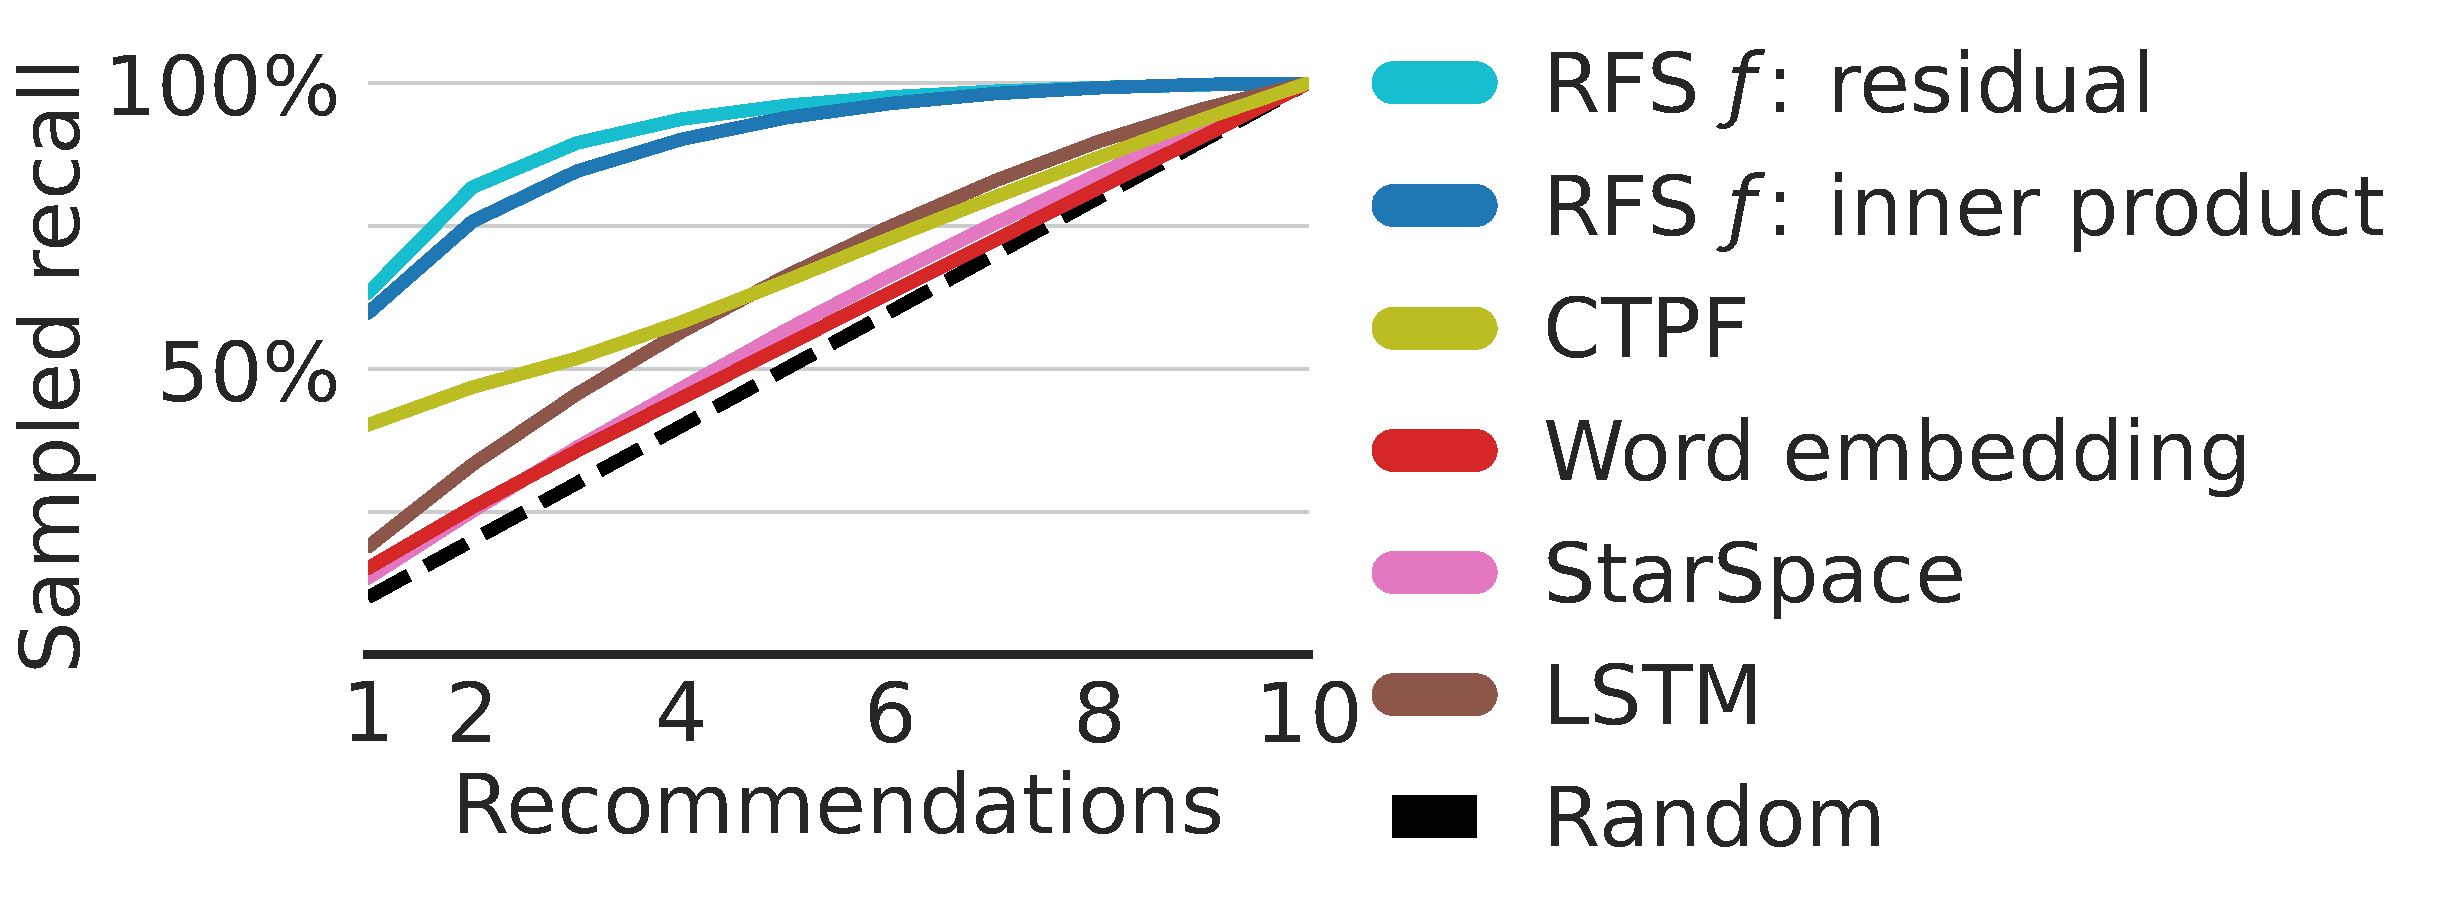
\includegraphics[width=0.7\linewidth]{ch-rfs/fig/meal-recall}
  \caption[\textsc{rfs} results on meal recommendation]{
  \textbf{\acrlong{rfs} models outperform competitors in meal
 recommendation in terms of sampled recall computed using \Cref{eq:sampled-recall}. Comparison models are described in \Cref{sec:models} (see \Cref{sec:appendix-empirical} for hyperparameters). The \gls{rfs} regression functions $f$ are defined in \Cref{eqn:rankfromsets,eqn:neural-network,eqn:residual} for the inner product, neural network, and residual models, respectively.}%
   % % The recommendation models
 % are trained on data from a food
    % tracking app as described in \Cref{sec:experiments_meals} and are evaluated
    % using the sampled recall metric, \Cref{eq:sampled-recall}. The inner
    % product, neural network, and residual regression functions for \acrlong{rfs}
    % are in \Cref{eqn:rankfromsets,eqn:neural-network,eqn:residual}
    }
  \label{fig:meal-recall}
  % \vspace{-0.5cm}
\end{figure}
\Cref{fig:meal-recall} shows the sampled recall: models in the \gls{rfs} class outperform others, such as permutation-marginalized recurrent neural networks and word embedding models. The residual \gls{rfs} model outperforms the \gls{rfs} inner product parameterization (and the equivalent LightFM model trained on the \gls{bpr} objective). The code released with~\citet{gopalan2014content-based} or \citet{wang2011collaborative} did not scale to this size of data, despite sufficient computing resources. This experiment further verifies \Cref {prop:maximizing-recall}: \gls{rfs} models can maximize recall.

Qualitatively, \gls{rfs} learns an interpretable representation of items, as
shown by nearest neighbors of meals in \Cref{tab:nearest_meals}. In this table,
we display breakfast, lunch, and dinner meals, alongside their nearest
neighbors. We find that the nearest neighbors are also breakfast, lunch, and
dinner meals respectively, showing that the attribute embeddings learned by the
model can be used to explore qualitative patterns in the learned latent space.
%%% Local Variables:
%%% mode: latex
%%% TeX-master: "set_recommendation"
%%% End:
% !TEX root = ../main.tex
% !TEX root = ../../main.tex
\newcommand{\y}{\faCheck}
% \newcommand{\y}{\checkmark}
\newcommand{\myscale}{0.1}
\newcolumntype{C}[1]{>{\centering}p{#1\linewidth}}
\begin{table*}[htb!]
  \begin{center}
  % \resizebox{1.0\textwidth}{!}{%
    \begin{tabular}{l
                    C{\myscale}
                    C{\myscale}
                    C{\myscale}
                    C{\myscale}
                    C{\myscale}
                    }
      \toprule
      Model & Attributes & Implicit & Scalable
      & Invariant & Evaluation \tabularnewline
      \midrule
      \acrlong{rfs} & \y & \y & \y & \y & \y \tabularnewline
      \acrshort{ctpf}, \citet{gopalan2014content-based}& \y & \y  &  & \y &\tabularnewline
      StarSpace, \citet{wu2018starspace:} &\y & \y &\y &\y
      &\tabularnewline
      LightFM, \citet{kula2015metadata} & \y & \y & \y & \y
      &\tabularnewline
      \acrshort{bpr}, \citet{rendle2009bpr:}&  & \y &  & & \y\tabularnewline
      \citet{wang2011collaborative} & \y & \y & & \y &
      \tabularnewline
     \citet{lian2018towards} & & & \y & & \tabularnewline
      \citet{dong2017a-hybrid}& \y & & & \y &\tabularnewline
      \citet{chen2017joint}&\y & &\y & &\tabularnewline
      \citet{bansal2016ask-the-gru:}&\y & \y & & &\tabularnewline
      \citet{xu2017tag-aware}& \y & & \y & \y &\tabularnewline
      % \citet{shi2012tfmap:} &\y & \y & & \y & \y\tabularnewline
      \citet{shi2012climf:} & & \y & & &\y \tabularnewline
      \citet{chen2018a-collective} & \y & \y & & \y & \tabularnewline
      \citet{liu2014recommending} & \y & & & \y & \y \tabularnewline
      \citet{cao2017embedding} & \y & &  & & \y \tabularnewline
      \citet{okura2017embedding-based} & \y & & \y & & \y \tabularnewline
%      \citett{zhang2018discrete} & \y & \y & \y & \y &\tabularnewline
      \bottomrule
    \end{tabular}
    % }
    \caption[\textsc{rfs}-related work]{
    \label{tab:background}
    \textbf{\acrlong{rfs} recommends items using attributes, and is
    trained to maximize the evaluation metric of recall.} Most
    methods we highlight leverage item attributes (Attributes); some require
    data in addition to the implicit feedback data of user-item interactions
    (Implicit). Few methods are scalable, as most models that use
    item side information require learning parameters for every item. Some
    models are invariant to permutation of the attributes (Invariant), and some
    enjoy a loss function that is connected to a recommender performance
    metric (Evaluation).}
    % \vspace{-0.5cm}
  \end{center}
\end{table*}
\section{Related Work}
We survey food recommender systems and recommendation models, focusing on models that leverage content information and scale to large numbers of users, items, and attributes.

Existing food recommendation systems focus on healthy recommendation~\citep{trattner2019an-evaluation,freyne2011recipe,khan2019personalized,yang2017yum-me:}, while \gls{rfs} focuses on the scalability challenge of meal recommendation. After training a recommendation model, it is possible to filter the recommendations by nutritional information to nudge users towards healthier eating habits~\citep{elsweiler2017exploiting}; such approaches can be used to include nutritional information into \gls{rfs} recommendations. When data is used in food recommender systems, it is usually recipe data~\citep{trattner2017food}; \gls{rfs} is designed to recommend meals using crowdsourced food consumption data which may accurately reflect user behavior~\citep{trattner2019what}.

We highlight several themes in research on recommendation models. We describe recommendation models that incorporate side information, models that recommend through classification, and models that optimize proxies of ranking metrics. This related work is summarized in~\Cref{tab:background}. We focus on deep learning-based and matrix factorization methods to include side information in recommendation models. Item side information can be modeled with deep representations or can be included in content-based matrix factorization models as an additional matrix. Some deep learning approaches scale to large datasets, but may not have objective functions tied to evaluation metrics, or may require data beyond user-item interactions~\citep{okura2017embedding-based}. Content-based matrix factorization methods require learning parameters for every item, and do not scale to data with large numbers of items~\citep{wang2011collaborative,gopalan2014content-based}, whereas \gls{rfs} scales and is tied to evaluation.

% \citep{zhang2017deep,bansal2016ask-the-gru:,lian2018towards,dong2017a-hybrid,chen2017joint,liang2018trsdl:,zuo2016tag-aware,xu2017tag-aware}
\paragraph{Deep Representations of Side Information.} Deep learning-based recommendation models incorporate side information in multiple ways \citep{zhang2017deep}. For example, items that have words as attributes can be represented using neural networks~\citep{bansal2016ask-the-gru:,chen2018a-collective} or embeddings~\citep{wu2018starspace:}. \gls{rfs} uses both embeddings and deep learning techniques such as residual networks~\citep{he2015deep} to include side information. \citet{lian2018towards} use an attention mechanism to weight recommendations according to available item and user side information, and \citet{dong2017a-hybrid} use denoising autoencoders to model side information in a deep recommendation model, but these methods require fitting parameters for every item and hence cannot scale. An example of a more efficient approach is the method in \citet{chen2017joint}, where embeddings are jointly learned for users, items, and item text for recommendation, but this method focuses on unsupervised pre-training of text representations. \gls{rfs} is complementary to such approaches, as the user, attribute, and item embeddings can be initialized using pre-training. Deep structured semantic models are designed for document retrieval given query words~\citep{huang2013learning,palangi2016deep}; it is unclear how to use this setup for recommending items with set-valued side information to users. There are several examples of `tag-aware' or `tag-based' deep recommendation models~\citep{liang2018trsdl:,zuo2016tag-aware}, such as \citet{xu2017tag-aware}, which focuses on data where users and items have different attributes and uses autoencoders to learn user, item, and attribute representations. \citet{xu2017tag-aware} uses a cosine similarity-based objective function which is not tied to a metric used to evaluate recommendation performance, whereas \gls{rfs} is tied to recall as shown in \Cref{prop:maximizing-recall}.
%, but this method requires collecting information about which items users decided not to consume.

\paragraph{Recommendation via Classification.} The framing of recommendation as classification has been around for a long time~\citep{basu1998recommendation}, and several works build deep learning-based classifiers for recommendation \citep{covington2016deep,cheng2016wide,guo2017deepfm:,he2017neural}. \citet{covington2016deep} focus on scalable inclusion of user and item attributes for video recommendation, \citet{cheng2016wide} jointly train generalized linear models and deep neural networks for recommendation, while \citet{guo2017deepfm:} use factorization machines to learn high- and low-order interactions of features. Our work is complementary to these approaches: \gls{rfs} focuses on scalable inclusion of set-valued side information, and provides theoretical undergirding to these recommendation models. We connect such models that rely on classification to optimal recall in \Cref{prop:maximizing-recall}. And if a specific architecture developed in these works is a permutation-invariant recommendation model, we proved that \gls{rfs} is a universal function approximator (\Cref{prop:universal-approximation}). So if performance is measured by recall, an \gls{rfs} model can converge to an optimal recommender.
%\citep{shi2014collaborative,gopalan2014content-based,wang2011collaborative,zhen2009tagicofi:,loepp2019interactive,bogers2018tag-based}

\paragraph{Matrix Factorization with Side Information.} While matrix factorization methods perform well in recommending items that have consumption data in the training set~\citep{hu2008collaborative,liang2016factorization}, they cannot recommend items that have not been consumed in the training data. Including side information in matrix factorization enables recommendation of these items with no consumption data. \citet{shi2014collaborative} survey several matrix factorization methods that leverage  side information. \citet{gopalan2014content-based} develop a Bayesian matrix factorization model for recommending items based on side information in the form of words in documents, and we compare \gls{rfs} to this method in \Cref{sec:rfs-experiments}. \citet{wang2011collaborative} develop a regression model that uses a topic model to incorporate side information into recommendations. There are also several `tag-based' or `tag-aware' content-based matrix factorization models~\citep{zhen2009tagicofi:,loepp2019interactive,bogers2018tag-based}. Such content-based matrix factorization methods maximize the conditional log-likelihood of the data (or a bound on the log-likelihood); optimizing these objective functions may not optimize an evaluation metric. These methods are not scalable to large numbers of items as they require learning unique parameters for every item. Specifically, such content-based matrix factorization methods require learning a matrix that has a row for every item. For items with attributes, it is often infeasible to store this matrix in memory or exploit efficient coordinate ascent optimization schemes that require processing this entire matrix. \gls{rfs}, however, is designed to scale to tens of millions of items, as we demonstrate empirically in \Cref{sec:rfs-experiments}.

\paragraph{Learning to Rank.} The learning to rank literature includes several recommendation models trained on objectives that approximate ranking-based evaluation metrics \citep{yu2018walkranker-fixed,liang2018top-n-rank:,rendle2009bpr:,song2018neural}, and some of these models include side information \citep{shi2012tfmap:,shi2012climf:,yuan2016optimizing,ying2016collaborative,cao2017embedding,okura2017embedding-based}. Such approaches can require data in addition to the user-item matrix, such as per-item parameters, or might use models whose output depends on the ordering of item attributes (making them infeasible for set-valued side information). In \Cref{sec:rfs-experiments}, we show that the ranking-based \gls{bpr} objective function~\citep{rendle2009bpr:,kula2015metadata} is in the \gls{rfs} class, so \Cref{prop:maximizing-recall} can help frame this related work. \citet{li2016a-relaxed} use an objective that is in the same class as \gls{bpr}, and other work bounds the \gls{bpr} objective~\citep{zhang2018discrete-deep}; these are also examples of \gls{rfs} models if a permutation-invariant architecture is specified and we study one such choice~\citep{kula2015metadata} in \Cref{sec:rfs-experiments}.
%%%%%%%%%%%%%%%%%%%%%%%%%%%%%%%%%%%%%%%%%%%%%%%%%%%%%%%%%%%%%%%%%%%%%%%%%%%%%%%%%%%%%%%%%%%%%%%%%%%%%%%%%%%%%%
% \subsection{Recommendation via ranking}
% We describe recommendation models trained on
% such loss functions and extensions that include side information.
% \paragraph{Learning to rank}
% The literature on learning to rank includes models that optimize proxies of
% evaluation metrics, such as mean average precision, mean reciprocal rank, or
% discounted cumulative gain~\citep{yu2018walkranker:,liang2018top-n-rank:}. Forb
% example, Bayesian personalized ranking models optimize a pairwise ranking
% objective function \citep{rendle2009bpr:} that trains the model to rank items a
% user consumed higher than items a user did not consume. This objective is a
% heuristic motivated by an analogy to the receiver operating characteristic; a
% model trained on this objective does not provably maximize this metric.
% \citet{song2018neural} extend Bayesian personalized ranking using deep neural
% networks, but do not model side information.
% \paragraph{Learning to rank with side information}
% Models that optimize proxies of ranking metrics that use side information
% include \citet{shi2012tfmap:}, where a smoothed approximation of mean average
% precision is used as a loss function. \citet{yuan2016optimizing} use a proxy of
% a ranking loss to fit a polynomial that models predictions of item consumption
% using item and side information features. \citet{ying2016collaborative} uses
% denoising autoencoders to represent item information in a model trained with a
% pairwise ranking loss. \citet{cao2017embedding} use a ranking loss to jointly
% learn embeddings of items and attributes; they focus on the case where users
% interact directly with both attributes and items with said attributes. All of
% these models require learning unique parameters for every item, and do not scale
% to large numbers of items. An example of a scalable method that uses the
% Bayesian personalized ranking criterion is in \citet{okura2017embedding-based},
% but this approach requires data with timestamps and negative item feedback.
% \paragraph{Order-invariant models.} Deep learning architectures have been
% developed for set-valued input. Such architectures are invariant to permutations
% of set elements and can approximate any order-invariant function
% \citep{zaheer2017deep,ravanbakhsh2017equivariance}. This work
% addresses regression whereas we focus on recommendation, and develop a negative
% sampling technique.
% %
% \citet{kumar2018representation} extend the order-invariant architectures to the
% problem of a set-valued response; we focus on set-valued input for which data is
% more readily available.
% %
% \citet{benson2018sequences} study the problem of predicting sets in a sequential
% order. The task is to predict attributes of a new item given the number of
% attributes. These attributes are modeled as coming from the attributes of the
% items a user has recently consumed. In contrast, we do not focus on temporal
% data and do not focus on repeated consumption of whole or partial copies of of
% items' sets of attributes.
% \paragraph{Ranking models.} Bayesian personalized ranking models optimize a
% ranking criterion \citep{rendle2009bpr:} that trains the model to rank items a
% user consumed higher than items a user did not consume. The criterion is
% motivated by an analogy to the receiver operating characteristic, but they do
% not prove that optimizing the criterion is equivalent to optimizing this metric.
% In our work, we prove (in \Cref{prop:maximizing-recall}) that our approach
% directly optimizes recall.
% %
% The Bayesian personalized ranking criterion has been extended to recommending
% news articles \citep{okura2017embedding-based}, but this approach requires the
% collection of observed (but not consumed) items. Our method applies to data
% where this additional information is not required.
% % c.f. https://data.princeton.edu/wws509/notes/c6s3
% \paragraph{Discrete choice econometrics models.} Conditional logit models are
% used in economics to study purchasing decisions \citep{mcfadden1973conditional},
% and may include characteristics of items such as attributes.
% %
% \citet{ruiz2017shopper:} develop a sequential model for discrete choice of
% consumer behavior. They focus on predicting additional attributes for an item
% conditioned on its existing attributes, whereas our task concerns ranking items
% given their attributes.
% %
% \citet{chiong2019random} use random projections to reduce the dimensionality of
% the choice set in a discrete choice model (the number of items). However, it is
% unclear whether their model scales: they study a dataset with a choice set of
% size $3$k. The choice set in the diet data we study has tens of millions of
% items.
% %
% \citet{overgoor2018choosing} develop a discrete choice model for graph-based
% data where the task is predicting new edges. They use negative sampling as
% training data for missing links in the graph, but do not address the case where
% nodes have set-valued attributes (that is the case we focus on).
% \paragraph{Deep learning-based recommender systems.} \citet{zhang2017deep}
% reviews several deep learning models for recommending items to users. However,
% these models are recommend items without leveraging side information as we do in
% this work.
% %
% For example, \citet{nguyen2018npe:} develop a model for recommendation with
% negative sampling, where the context items are other items a user has consumed.
% (They not study the case where items are represented by sets of attributes.)
% %
% \citet{trofimov2018inferring} use a ranking loss with negative sampling for
% learning embeddings to predict attributes of an item conditional on existing
% attributes. Our task differs in that we aim to recommend items conditional on
% their full set of attributes.
% %
% \citet{chen2017joint} study the task of ranking text for users by incorporating
% different unsupervised representations of text. They do not address the task of
% recommending items that are represented by sets of attributes as we focus on
% here.
% \paragraph{Negative sampling in recommender systems.}
% \citet{chen2017on-sampling} analyze computational tradeoffs of different
% negative sampling strategies for recommender systems. Their work is
% complementary to ours, and could speed up the training of our model.

% !TEX root = rankfromsets.tex
\section{Discussion}
The task of recommending items with attributes is difficult for several reasons. It is unclear how to incorporate set-valued side information into models that scale to large numbers of items and attributes. In addition, existing recommendation models that leverage item attributes (for example, content-based matrix factorization) are not directly tied to evaluation metrics. We developed \gls{rfs}, a class of scalable recommendation models for items with attributes. Theoretically, we showed that optimizing the \gls{rfs} objective optimizes recall, and that \gls{rfs} can approximate permutation-invariant recommendation models including content-based matrix factorization. Empirically, models in the \gls{rfs} class outperform competing models and scale to large datasets, such as our motivating problem of meal recommendation for 55k users who consume 16M meals.

How well does binary classification perform for other ranking-based recommendation metrics, such as non-discounted cumulative gain? Analyzing this question is more difficult, and we leave this to future work. For generalization theory, we conjecture that a different loss function should allow a similar proof to \Cref{prop:maximizing-recall}. With sufficient data, \gls{rfs} can learn arbitrary distributions of users consuming items with attributes. But performance on finite data can vary, and developing generalization theory for \gls{rfs} remains an open question.

% \paragraph{Simple theory and implementation} It is surprising that \gls{rfs}
% outperforms the collaborative topic Poisson factorization model in
% \citet{gopalan2014content-based}, as \gls{rfs} is a much simpler model.
% \gls{rfs} does not require approximate posterior inference as in \gls{ctpf}, but
% mere binary classification. \gls{rfs} is also simpler in terms of
% implementation: a scalable example is a few dozen lines of python in
% \Cref{sec:code}, compared to several thousand lines of C++ released by the
% authors of \gls{ctpf}.

% \paragraph{Architectures} There is a wealth of deep learning models that can be
% used to parameterize \gls{rfs}. For example, attention-based transformer
% networks can operate on set-valued input~\citep{lee2018set-transformer} and are
% an interesting choice of architecture for \gls{rfs}.

% larger batch sizes on cpu
% For good performance on the arXiv dataset, large batch sizes were necessary. We
% were limited in batch size due to our use of a GPU. Reimplementing the model in
% C++ would free the model from GPU memory restrictions, enabling larger batch
% sizes and better performance.
% optimization: ctpf benefits from coordinate ascent
% \paragraph{Optimization} Collaborative topic Poisson factorization as the latter
% enjoys an efficient optimization algorithm. The conjugacy properties of the
% matrix factorization model permit coordinate ascent and fast convergence in few
% iterations. The nonconvex objective function that \gls{rfs} relies on may be
% amenable to certain optimization techniques, such as dual coordinate
% ascent~\citep{yu2011dual}, and we leave this to future work.

% \paragraph{Side information} The \gls{rfs} model can easily accommodate various
% metadata about users, items, or attributes. Attribute-level or user-level side
% information is particularly interesting, and when available, should lead to
% improved recommendation performance.

% % we did not study regularization
% \paragraph{Regularization} Further performance gains from regularizing \gls{rfs}
% are also interesting avenues for future work. L2 regularization for sparsity and
% dropout for decorrelation may yield improvements.

% RMSProp~\citep{graves2013generating} was also tested when fitting
% \gls{rfs} to the arXiv data. This optimizer outperformed
% collaborative topic Poisson factorization in terms of both in-matrix precision
% and recall, but matched the performance of the matrix factorization model in
% terms of out-matrix precision and recall. This means there are tradeoffs of
% using different optimizers that depend on the data and evaluation metrics of
% interest.
% initializing to word2vec
% \paragraph{Pretrained embeddings} We note that the word embedding baseline
% performed slightly worse as collaborative topic Poisson factorization, which is
% surprising given that the word embedding model is much simpler. Further
% performance gains in \gls{rfs} should be possible by initializing user and item
% attribute embeddings to pretrained word embeddings as in \citet{chen2017joint}.

% % gap in prop 2
% \paragraph{Theory (approximation)} \Cref{prop:universal-approximation} means
% that \gls{rfs} can approximate the output of any order-invariant model
% such as matrix factorization. However, there is no guarantee that fit with
% maximum likelihood estimation using the objective in \Cref{eq:objective},
% \gls{rfs} \emph{will} approximate a specific model. We leave the development of
% such approximation techniques to future work.
% out-of-vocabulary words
% An open question is how to account for new attributes, for example in
% crowdsourced data. An extension of this work would be to combine it with
% character-level embeddings as in \citep{bojanowski2017enriching} to enable the
% model to better perform recommendations for out-of-vocabulary attributes.
% can we optimize metrics other than recall?


% \section*{Acknowledgments}
% % and emotional support
% J.A. is grateful to Mark Goldstein and Bharat Srikisan for helpful
% discussions, and to Kyle Cranmer
% and the Center for Data Science at New York University for desk space. The
% experiments presented in this article were performed on computational resources
% supported by the Princeton Institute for Computational Science and Engineering
% and the Office of Information Technology's High Performance Computing Center and
% Visualization Laboratory at Princeton University.

%%% Local Variables:
%%% mode: latex
%%% TeX-master: "set_recommendation"
%%% End:
% !TEX root = ../main.tex
% \appendix
\section{Appendix}
\subsection{Empirical Study Hyperparameters}
\label{sec:appendix-empirical}

Experiments for \gls{rfs}, LightFM, and recurrent neural network models are run on a cluster with Tesla P100 GPUs using PyTorch; all other experiments are performed on a 20-core computer.

\paragraph{Hyperparameters for Word Embedding Model and StarSpace.} For the word embedding model and StarSpace, we use the software packages released alongside the respective papers~\citep{bojanowski2017enriching,wu2018starspace:} with recommended hyperparameters, and grid search over embedding sizes of $\{128, 256, 512, 1024\}$ for both datasets.

\paragraph{Hyperparameters for LightFM.} On both datasets, LightFM with the logistic objective reported in \citet{kula2015metadata} performs poorly and we omit these results. \citet{kula2015metadata} does not use the \gls{bpr} objective in the paper; nevertheless, we study LightFM with the \gls{bpr} objective (this variant is unpublished, yet implemented in the code released in \citep{kula2015metadata}) and use the same hyperparameters as \gls{rfs} for comparison.

\subsection{Recommending Research Papers}
\label{sec:hyper-arxiv}
\paragraph{Hyperparameters for \acrshort{rfs}.} We test the stochastic gradient descent algorithm with and without momentum \citep{sutskever2013on-the-importance}. We use a linear learning rate decay that decays to zero in the maximum number of iterations, $200$k. We perform a grid search over learning rates of $\{1, 5, 10, 15, 25\}$ and momenta of $\{0.5, 0.9, 0.95, 0.99\}$. The minibatch size is set to $2^{16}$. We use a single negative sample per datapoint, sampled uniformly over the entire dataset; such corpus sampling is defined in \Cref{sec:rankfromsets}. As the number of items is small relative to the larger diet tracking data, the item intercept function is simply a scalar for every item, and the item embedding function learns item embeddings. To match the hyperparameters in \citet{gopalan2014content-based}, we set the dimensionality of user and item embeddings to $100$. Evaluation is performed every $20$k iterations.

\paragraph{Hyperparameters for Recurrent Neural Network Models.} We implement the model in \citet{bansal2016ask-the-gru:} using PyTorch and match the hyperparameters where possible. We test \gls{gru} cells and \gls{lstm} cells with the objective function in \Cref{eq:objective}. The model has access to full sequence information, unlike \gls{rfs}, as abstracts of research papers have meaningful sequence information (marginalizing using \Cref{eq:rnn} would destroy information and decrease performance). The attribute embedding size is fixed to $100$ to match the other models and attribute embeddings are initialized to word embeddings pretrained on all 636k document abstracts as in \citet{bansal2016ask-the-gru:}, using the word embedding implementation in \citet{bojanowski2017enriching}. The first layer of the recurrent neural network is bidirectional and of hidden size $400$, the second layer is unidirectional and of hidden size $200$, and dropout is used with the same settings as in \citet{bansal2016ask-the-gru:}. Evaluation is performed every $20$k iterations. We grid search over learning rates of $\{10^{-1}, 10^{-2}, 10^{-3}, 10^{-4}\}$ with the Adam optimizer \citep{kingma2015adam:} and batch sizes of $\{64, 128, 256, 512, 1024, 4096, 8192\}$. As evaluation is much more expensive for sequence models, we randomly select a subset of $100$ users from the held-out set of 10k users. If validation performance does not improve, we reload the best parameters and optimizer states, and divide the learning rate by half. In both experiments, \gls{lstm} cells outperformed \gls{gru} cells.

\subsection{Recommending Meals}
\paragraph{Hyperparameters for \gls{rfs}.} The embedding size is set to $128$. For the neural network and residual models in \Cref{eqn:neural-network,eqn:residual} the number of hidden layers is two, and the number of hidden units is set to $256$ with rectifier nonlinearities. The item embeddings $g(x_m)$, and item intercepts $h(x_m)$, are computed as the mean of learned food embeddings and intercepts, respectively. We use the RMSProp optimizer in \citet{graves2013generating} and grid search over the learning rates $\{10^{-2}, 10^{-3}, 10^{-4}, 10^{-5}\}$. We use a batch size of $64$ and a single negative sample for every datapoint in a minibatch (batch sampling is defined in \Cref{sec:rankfromsets}). Evaluation is performed every $50$k iterations.

\paragraph{Hyperparameters for Permutation-marginalized Recurrent Neural Networks.} We use the same settings as described in \Cref{sec:hyper-arxiv}, but the data in this case has no sequence information so we use \Cref{eq:rnn} to average predictions of the model in \citet{bansal2016ask-the-gru:} over permutations. Evaluation for sequence models is already prohibitive, so for every item in a minibatch we sample a single permutation of attributes to approximate the sum over permutations in \Cref{eq:rnn}. We use a single negative sample per datapoint (minibatch sampling), and set the embedding and hidden state sizes to $128$. We use the Adam optimizer~\citep{kingma2015adam:} and grid search over the same learning rates, learning rate decay, and batch sizes as in \Cref{sec:hyper-arxiv}, with evaluation every 1k iterations.

\subsection{Generalization Simulation Study}
\label{sec:simulation}
% In this simulation, the regression function $f$ was the square kernel between
% the user embedding $\theta_u$ and the mean of item attribute embeddings
% ${\beta_j: j \in x^+_m}$. For a fair comparison, the regression functions in
% \Cref{eqn:rankfromsets,eqn:neural-network,eqn:residual} were chosen to have the
% same number of parameters. For data generated using the square kernel, the
% residual and deep parameterizations outperformed the inner product
% parameterization.
\Cref{prop:universal-approximation} is a universal function approximation theorem in the regime of infinite data. With finite data and a finite number of parameters, the optimal parameterization of \gls{rfs} is dependent on the data-generating distribution. From \Cref{fig:meal-recall}, the inner product \gls{rfs} parameterization outperforms the neural network parameterization. We demonstrate a simulated dataset where this order is reversed, to motivate the exploration of novel architectures. Recall that observations of user-item interactions are generated by a Bernoulli distribution with logit function $f$. We describe a choice of logit function $f$ that leads to the residual and deep architectures in \Cref{eqn:residual,eqn:neural-network} outperforming the inner product architecture in \Cref{eqn:rankfromsets} in terms of predictive performance. We will release all code required to replicate this experiment.
\begin{enumerate}
  \item \textbf{For every user $u$:} Draw user embedding $\theta_u \sim \textrm{Normal}(0, \mbI)$.
  \item \textbf{For every attribute $j$:} Draw attribute embedding $\beta_j \sim \textrm{Normal}(0, \mbI)$.
  \item \textbf{For every item $m$:}
    \begin{enumerate}
    \item Draw item topics $\theta_m \sim \textrm{Dirichlet}(\alpha)$
    \item Draw number of item attributes $M \sim \textrm{Poisson}(\lambda)$
    \item Draw nonzero item attributes $x_m \sim \textrm{Multinomial}(M, \theta_m)$.
    \end{enumerate}
  \item \textbf{For every user, item:} $\yum \sim \textrm{Bernoulli}\left(\yum; \sigma(f(\theta_u, x_m)\right)$.
\end{enumerate}
The logit function $f$ is the square kernel:
$$f(\theta_u, x_m) = \left(\theta_u^\top \frac{1}{|x_m|}\sum_{j \in x_m}
  \beta_j\right)^2.$$
The output of $f$ is standardized across users and centered at $7$ to achieve sparse user-item observations.

For this simulation study, we set the Dirichlet parameter to be $\alpha=0.01$ and the Poisson rate to be $\lambda=20$. We generate data for $1$k users, $5$k item attributes, $30$k items, and hold out $100$ users for each of the validation and test sets. The embedding sizes are fixed to $100$, and for parameterizations with neural networks two hidden layers are used with rectifier nonlinearities. The hidden size of models with neural networks is chosen so the total number of parameters matches the number of parameters in the inner product model. We fix the momentum to $0.9$~\citep{sutskever2013on-the-importance} and grid search over stochastic gradient descent learning rates of ${10, 1, 0.1, 0.01}$ and over two learning rate decay schedules. The first linear learning rate decay goes to zero over $100$k iterations, while the second divides the learning rate by $10$ if the validation in-matrix recall does not improve (evaluation is performed every $500$ iterations). We run the grid search on one instance of data generated from this model. We regenerate data $30$ times and average results over these synthetic datasets, using the best performing hyperparameters for each model trained on the first instance.

% !TEX root = ../../main.tex
\begin{table}[tb!]
\sisetup{table-figures-uncertainty=1}
\centering
\begin{tabular}{
  l
  S[table-format=1.2,
   table-figures-uncertainty=1]
  S[table-format=1.2,
  table-figures-uncertainty=1]
  S[table-format=1.2,
  table-figures-uncertainty=1]
  }
  \toprule
   & {Inner product} & {Deep} & {Residual} \\
  \midrule
  Recall & 0.29 \pm 0.15 & 0.32 \pm 0.14 & 0.33 \pm 0.18 \\
  \bottomrule\\
\end{tabular}
\caption[\textsc{rfs} simulation study]{\textbf{A simulation study demonstrating that the choice of     parameterization of \acrlong{rfs} is data-dependent.} We report the   in-matrix recall averaged over 100~users, over 30~replications of the simulation. The residual model in \Cref{eqn:residual}   outperforms the deep model in \Cref{eqn:neural-network} and the inner product   model in \Cref{eqn:rankfromsets}.} \label{tab:simulation}
\end{table}
The results in \Cref{tab:simulation} demonstrate that the residual model outperforms both the deep and inner product architectures for data generated by the above generative process. This shows that the choice of architecture in \gls{rfs} is data-dependent and leads to considering when a \gls{rfs} recommendation model supports generalization. To ensure that the model does not overfit as new users or items are included in the training data, we need to compare the number of parameters to the number of datapoints. A model with parameters the size of the training data can overfit by memorizing the training data. For generalization to be possible, overfitting can be avoided if the number of parameters grows slower than the size of the data. The technical backing for this comes from asymptotic statistics and the concept of sieved likelihoods. Specifically, the maximum likelihood estimation procedure with the objective function in \Cref{eq:objective} can be replaced by maximization of a sieved likelihood function. The `sieve' refers to filtering information as the number of parameters (in this case, the number of parameters in user and item representations) grows with the number of observations. The sieved likelihood function enables the analysis of asymptotic behavior as the number of users grows $U\rightarrow \infty$ and the number of items grows $I\rightarrow \infty$. An example of a technique to grow the number of parameters in a way that supports generalization is given in Chapter 25 of \citet{vaart1998asymptotic}.

\clearpage
\subsection{Code}
\label{sec:code}
We give an example implementation of \acrlong{rfs} with the inner product regression function in \Cref{eqn:rankfromsets} in python with the PyTorch package. This implementation is easy to port to new applications and achieves state-of-the-art results in \Cref{sec:rfs-experiments}.
\lstinputlisting[language=Python]{ch-rfs/code.py}

% !TEX root = altosaar-2020-thesis.tex
\chapter{Proximity Variational Inference}
\label{ch:pvi}
\lettrine[image=true,lines=3]{design/P}{reviously}, \Cref{ch:hvm,ch:rfs} highlighted how consideration of the problem structure enabled efficient probabilistic modeling solutions to applied questions in physics and recommender systems. Can problem structure be of use at a higher level, in an inference algorithm that can be re-used across probability models? We develop \acrlong{PVI} in this chapter, which enables \acrlong{vi} to leverage information about variational approximations during optimization to improve the accuracy of inference.
% !TEX root = ../main.tex
\section{Introduction}
\label{sec:pvi-introduction}
\Gls{VI} is a powerful method for probabilistic modeling.  \gls{VI} uses optimization to approximate difficult-to-compute conditional distributions~\citep{jordan1999introduction}.  In its modern incarnation, it has scaled Bayesian computation to large data sets~\citep{hoffman2013stochastic}, generalized to large classes of models~\citep{kingma2014autoencoding,ranganath2014black,Rezende:2015}, and has been deployed as a computational engine in probabilistic programming systems~\citep{DBLP:journals/corr/MansinghkaSP14,Kucukelbir:2015,tran2016edward}.

Despite these significant advances, however, \gls{VI} has drawbacks. For one, it tries to iteratively solve a difficult nonconvex optimization problem and its objective contains many local optima. Consequently, \gls{VI} is sensitive to initialization and easily gets stuck in a poor solution.  We develop a new optimization method for \gls{VI} and show that it finds better optima.

Consider a probability model $p(\mbz,\mbx)$ and the goal of calculating the posterior $p(\mbz \mid \mbx)$. The idea behind \gls{VI} is to posit a family of distributions over the hidden variables $q(\mbz ; \mblambda)$ and then fit the variational parameters $\mblambda$ to minimize the \gls{KL} divergence between the approximating family and the exact posterior, $\textsc{kl}(q(\mbz ; \mblambda) || p(\mbz \mid \mbx))$. The \gls{KL} is not tractable so \gls{VI} optimizes a proxy.  That proxy is the
\gls{ELBO},
\begin{align}
\cL(\mblambda) = \E[\log p(\mbz,\mbx)] - \E[\log q(\mbz ; \mblambda)],
\label{eq:ELBO}
\end{align}
where expectations are taken with respect to $q(\mbz ; \mblambda)$. Maximizing the \gls{ELBO} with respect to $\mblambda$ is equivalent to minimizing the \gls{KL} divergence.
% !TEX root = ../main.tex
\begin{figure*}[t]
\centering
\begin{subfigure}{0.49\linewidth}
  \centering
  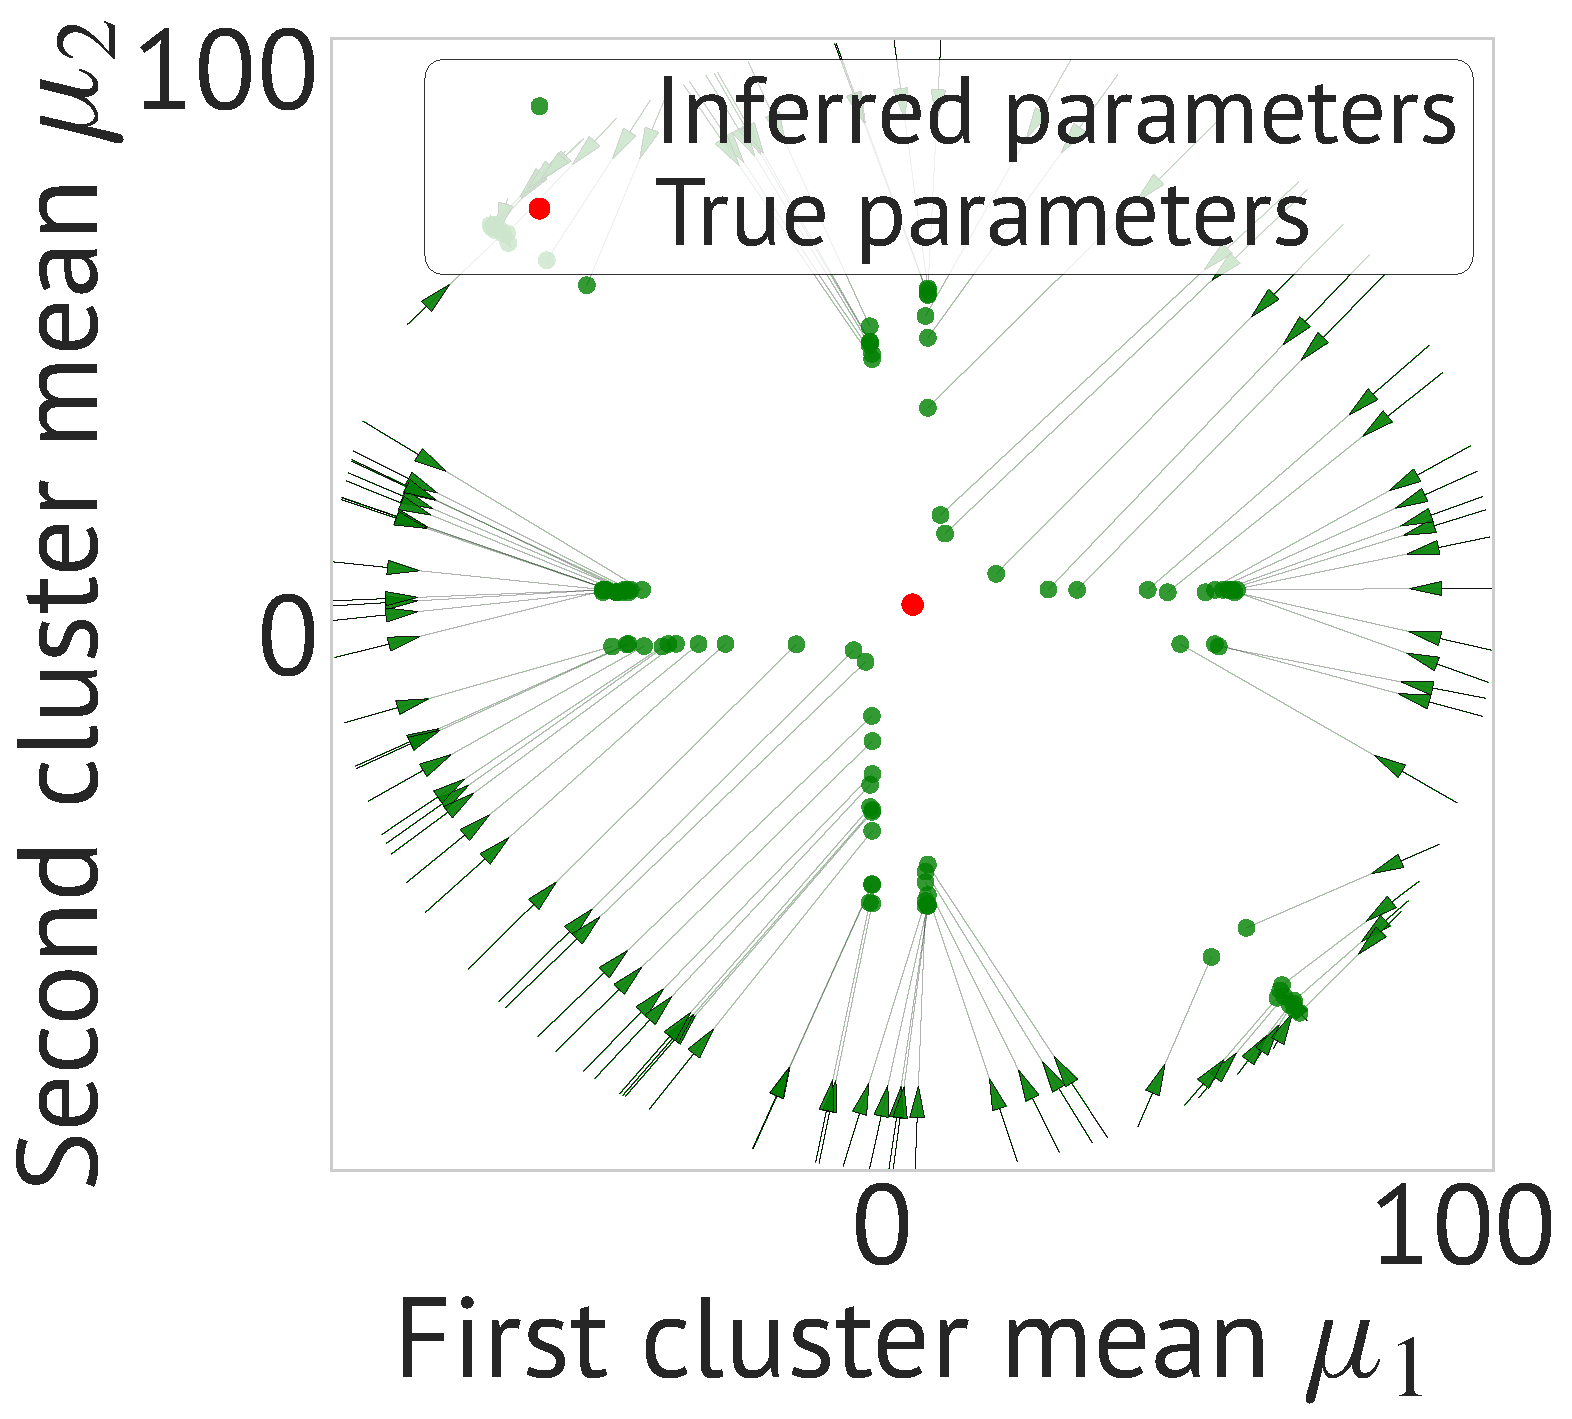
\includegraphics[width=0.8\linewidth]{ch-pvi/img/toy_vanilla}
  \label{fig:bernoulli_vanilla}
  \caption{Variational Inference}
\end{subfigure}
\begin{subfigure}{0.49\linewidth}
    \centering
    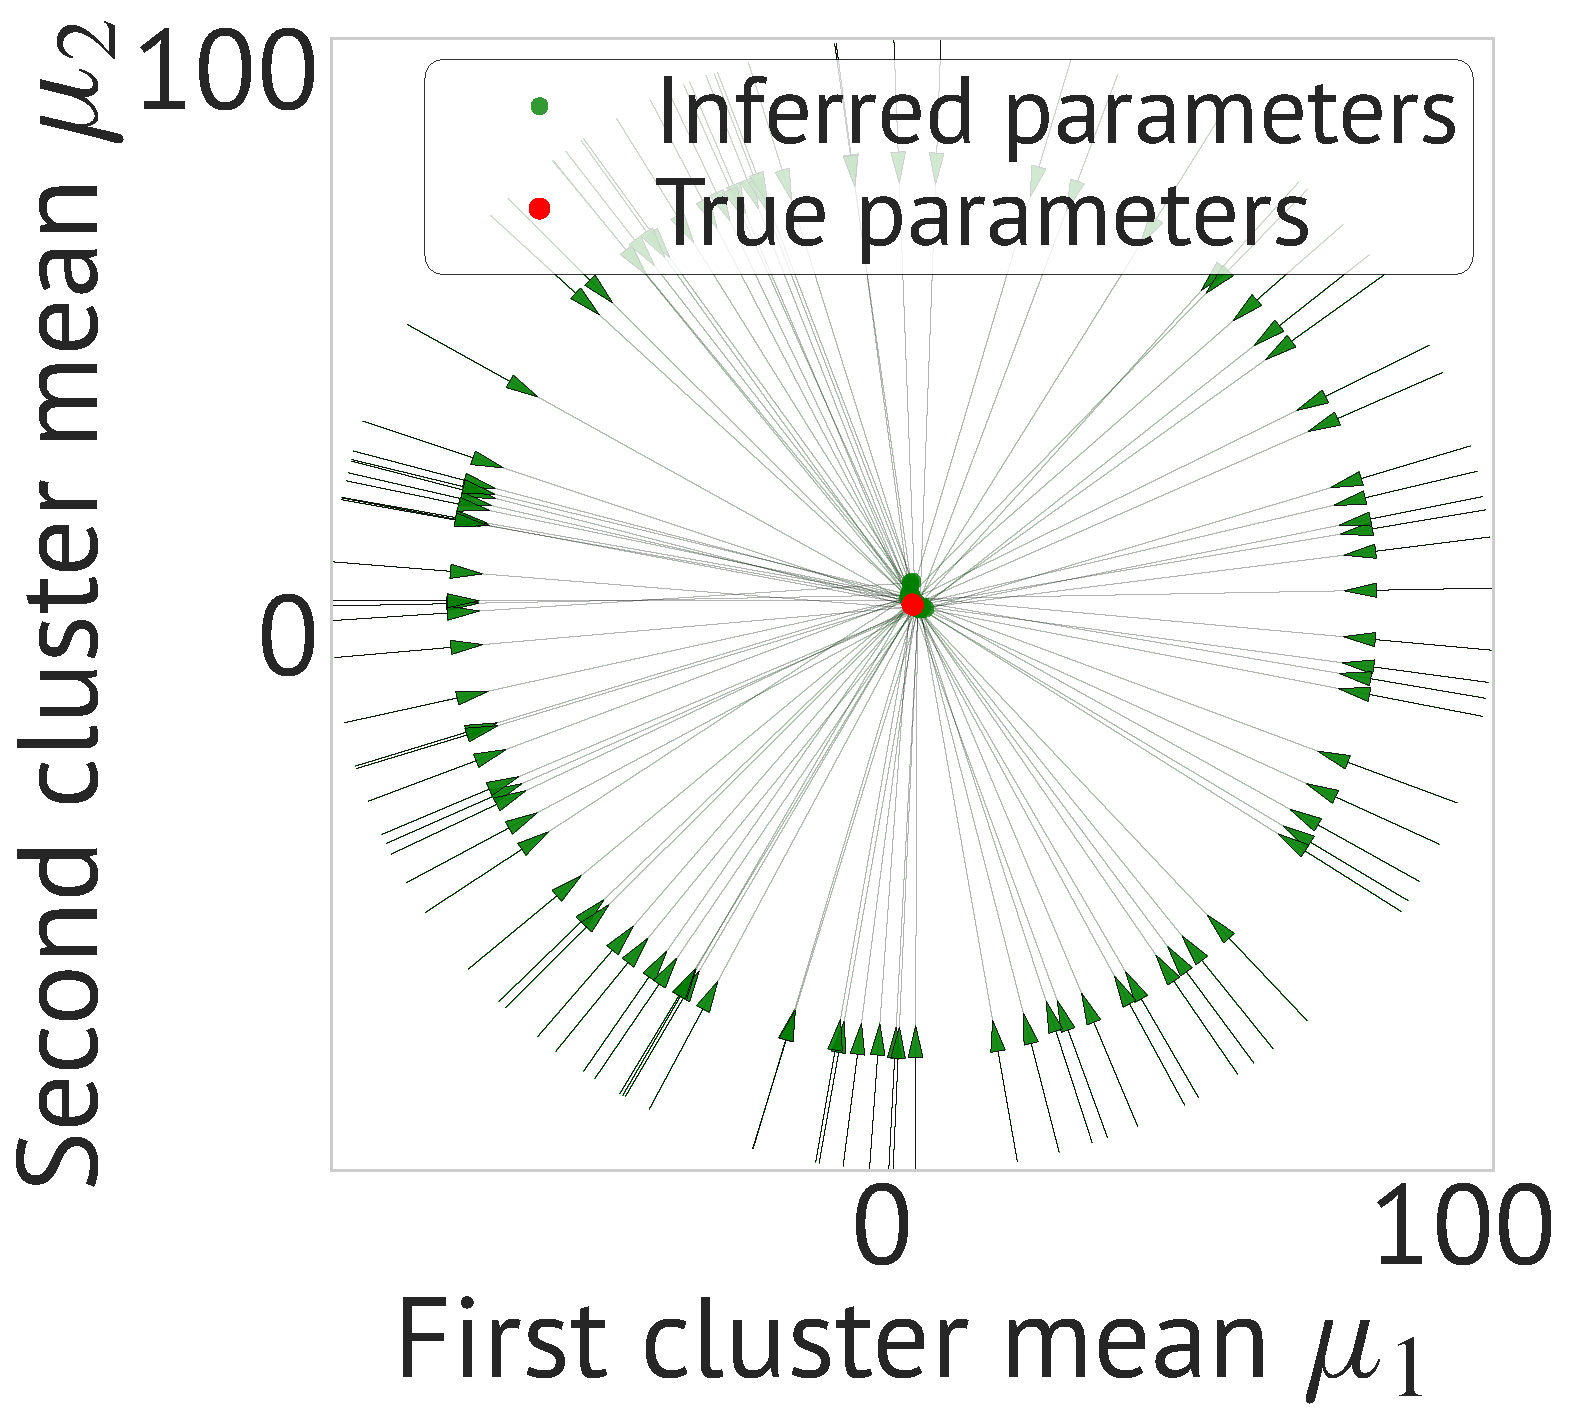
\includegraphics[width=0.8\linewidth]{ch-pvi/img/toy_global}
    \label{fig:bernoulli_global}
    \caption{Proximity \gls{vi}, \Cref{algo:global}}
\end{subfigure}
\caption[\textsc{pvi} makes \textsc{vi} robust to poor initialization]{
\textbf{\Acrlong{PVI} is robust to bad initialization.} We study a Bernoulli factor model. Model parameters are randomly initialized on a ring around the known true parameters (in red) used to generate the data. The arrows start at these parameter initializations and end at the final parameter estimates (shown as green dots). \textbf{(a)} Variational inference with gradient ascent suffers from multiple local optima and cannot reliably recover the truth. \textbf{(b)} \gls{PVI} with an entropy proximity statistic reliably infers the true parameters using \Cref{algo:global}.
}
\label{fig:bernoulli_arrows}
\end{figure*}
The issues around \gls{VI} stem from the \gls{ELBO} and the iterative algorithms used to optimize it. When the algorithm zeroes (or nearly zeroes) some of the support of $q(\mbz ; \mblambda)$, it becomes hard to later ``escape,'' i.e., to add support for the configurations of the latent variables that have been assigned zero probability~\citep{mackay2003information, Burda2016}. This leads to poor local optima and to sensitivity to the starting point, where a misguided initialization will lead to such optima. These problems happen in both gradient-based and coordinate ascent methods. We address these issues with \glsreset{PVI} \gls{PVI}, a variational inference algorithm that is specifically designed to avoid poor local optima and to be robust to different initializations.

\gls{PVI} builds on the proximity perspective of gradient ascent.  The proximity perspective views each step of gradient ascent as a constrained minimization of a Taylor expansion of the objective around the previous step's parameter~\citep{Spall:2003,boyd2004convex}.  The constraint, a \textit{proximity constraint}, enforces that the next point should be inside a Euclidean ball of the previous.  The step size relates to the size of that ball. We construct \gls{PVI} by questioning whether such a Euclidan distance-based constraint is appropriate, and whether other notions of proximity may be useful in constraining gradient ascent steps.

In \gls{VI}, a constraint on the Euclidean distance means that all dimensions of the variational parameters are equally constrained. We posit that this leads to problems; some dimensions need more regularization than others. For example, consider a variational distribution that is Gaussian.  A good optimization will change the variance parameter more slowly than the mean parameter to prevent rapid changes to the support.  The Euclidean constraint cannot enforce this. Furthermore, the constraints enforced by gradient descent are transient; the constraints are relative to the previous iterate---one poor move during the optimization can lead to permanent optimization problems.

To this end, \gls{PVI} uses proximity constraints that are more meaningful to variational inference and to optimization of probability parameters.  A constraint is defined using a proximity statistic and distance function. As one example, we consider a constraint based on the entropy proximity statistic. This limits the change in entropy of the variational approximation from one step to the next.  Consider again a Gaussian approximation. The entropy is a function of the variance alone and thus the entropy constraint counters the pathologies induced by the Euclidean proximity constraint. We also study constraints built from other proximity statistics, such as those that penalize the rapid changes in the mean and variance of the approximate posterior.

\Cref{fig:bernoulli_arrows} provides an illustration of the advantages of \gls{PVI}.  Our goal is to estimate the parameters of a factor analysis model with variational inference, i.e., using the posterior expectation under a fitted variational distribution.  We run variational inference $100$ times, each time initializing the estimates (the model parameters) to a different position on a ring around the truth.

In the figure, red points indicate the true value. The start locations of the green arrows indicate the initialized estimates. Green points indicate the final estimates, after optimizing from the initial points. Panel (a) shows that optimizing the standard \gls{ELBO} with gradients leads to poor local optima and misplaced estimates.  Panel (b) illustrates that regardless of the initialization, \gls{PVI} with an entropy proximity statistic finds estimates that are close to the true value.

The rest of this chapter is organized as follows. \Cref{sec:variational_inference} reviews variational inference and the proximity perspective of gradient optimization.  \Cref{sec:pvi} derives \gls{PVI}; we develop four proximity constraints and two algorithms for optimizing the \gls{ELBO}. We study four models in \Cref{sec:pvi-experiments}: a Bernoulli factor model, a sigmoid belief network \citep{Mnih:2016:VIM:3045390.3045621}, a variational autoencoder~\citep{kingma2014autoencoding,rezende2014stochastic}, and a deep exponential family model of text~\citep{ranganath2015deep}. \gls{PVI} outperforms classical methods for variational inference.

% !TEX root = ../main.tex
\parhead{Related Work.}  Recent work has proposed several related algorithms. \citet{khan2015kullback} and \citet{Theis2015} develop a method to optimize the \gls{ELBO} that imposes a soft limit on the change in \gls{KL} of consecutive variational approximations. This is equivalent to \gls{PVI} with identity proximity statistics and a \gls{KL} distance function. \citet{Khan:2016:FSV:3020948.3020982} extend both prior works to other divergence functions. Their general approach is equivalent to \gls{PVI} identity proximity statistics and distance functions given by strongly-convex divergences. Compared to prior work, \gls{PVI} generalizes to a broader class of proximity statistics. We develop proximity statistics based on entropy, \gls{KL}, orthogonal weight matrices, and the mean and variance of the variational approximation.

The problem of model pruning in variational inference has also been studied and
analytically solved in a matrix factorization model in \citet{nakajima2013}---this method is model-specific, whereas \gls{PVI} applies to a much broader class of latent variable models. Finally, deterministic annealing~\citep{Katihara:2008} consists of adding a temperature parameter to the entropy term in the \gls{ELBO} that initialized to a large value then annealed to unity during inference. This is similar to \gls{PVI} with the entropy proximity statistic which keeps the entropy stable across iterations. Deterministic annealing enforces global penalization of low-entropy configurations of latent variables rather than the smooth constraint used in \gls{PVI}, and cannot accommodate the range of proximity statistics we design in this work.
\section{Variational Inference}
\label{sec:variational_inference}

Consider a model $p(\mbx, \mbz)$, where $\mbx$ is the observed data and $\mbz$ are the latent variables.  As described in \Cref{sec:pvi-introduction}, \gls{VI} posits an approximating family $q(\mbz; \mblambda)$ and maximizes the \gls{ELBO} in \Cref{eq:ELBO}. Solving this optimization is equivalent to finding the variational approximation that minimizes \gls{KL} divergence to the exact posterior \citep{jordan1999introduction,wainwright2008graphical}.

\subsection{Gradient Ascent has Euclidean Proximity}
\label{sec:euclidean_proximity}
Gradient ascent maximizes the \gls{ELBO} by repeatedly following its gradient.  One view of this algorithm is that it repeatedly maximizes the linearized \gls{ELBO} subject to a proximity constraint on the current variational parameter~\citep{Spall:2003}. The name `proximity' comes from constraining subsequent parameters to remain close in the proximity statistic. In gradient ascent, the proximity statistic for the variational parameters is the identity function $f(\mblambda) = \mblambda $, and the distance function is the square difference.

Let $\mblambda_t$ be the variational parameters at iteration $t$ and $\rho$ be a constant. To obtain the next iterate $\mblambda_{t+1}$, gradient ascent maximizes the linearized \gls{ELBO},
\begin{align}
  \label{eq:linearized-elbo}
  % \begin{split}
    U(\mblambda_{t+1}) = %&
    \cL(\mblambda_t) +
    \nabla\cL(\mblambda_t)^\top(\mblambda_{t+1}-\mblambda_t) %\\
     - %&
    \frac{1}{2\rho} (\mblambda_{t+1}-\mblambda_t)^\top
    (\mblambda_{t+1}-\mblambda_t).
  % \end{split}
\end{align}
Specifically, this is the linearized \gls{ELBO} around $\mblambda_t$, subject to $\mblambda_{t+1}$ being close to $\mblambda_t$ in squared Euclidean distance.

Finding the $\mblambda_{t+1}$ which maximizes \Cref{eq:linearized-elbo} yields
\begin{align}
  \mblambda_{t+1} = \mblambda_t + \rho
  \nabla\cL(\mblambda_t). \label{eq:standard_update}
\end{align}
This is the familiar gradient ascent update with a step size of $\rho$. The step size $\rho$ controls the radius of the Euclidean ball which demarcates valid next steps for the parameters.  Note that the Euclidean constraint between subsequent iterates is implicit in all gradient ascent algorithms.

\subsection{An Example where Variational Inference Fails}
\label{sec:bernoulli_factor_model}
We study a setting where variational inference suffers from poor local optima. Consider a factor model, with Bernoulli latent variables and Gaussian likelihood:
\begin{align}
z_{ik}~&\sim~\textrm{Bernoulli}(\pi) \\
x_i~&\sim~\textrm{Gaussian}\left(\mu = \textstyle \sum_k z_{ik}
        \mu_k, \sigma^2=1\right).
\end{align}
This is a ``feature'' model of real-valued data $x$; when one of the features is on (i.e., $z_{ik}=1$), the $i$th mean shifts according the that feature's mean parameter (i.e., $\mu_{k}$).  Thus the binary latent variables $z_{ik}$ control which cluster means $\mu_k$ contribute to the distribution of $x_i$.

The Bernoulli prior is parametrized by $\pi$; we choose a Bernoulli approximate posterior $q(z_k;\lambda_k)~=~\textrm{Bernoulli}(\lambda_{k})$.  A common approach to \gls{VI} is coordinate ascent~\citep{bishop2006pattern}, where we iteratively optimize each variational parameter.  The optimal variational parameter for $z_{ik}$ is
\begin{align}
  \label{eq:z_update} \lambda_{ik} \propto
   \exp \left\{\E_{-z_{ik}} \left[- \frac{1}{2\sigma^2}(x_i -
    \sum_{j} z_{ij} \mu_j)^2\right]\right\}.
\end{align}
We can use this update in a variational expectation-maximization setting.  The
corresponding gradient for $\mu_k$ is
\begin{align}
  \label{eq:mu-gradient}
  \frac{\partial \cL}{\partial\mu_k}
  &= -
    \frac{1}{\sigma^2}\sum_i
    \left(-x_i \lambda_{ik} + \lambda_{ik} \mu_k
    + \lambda_{ik} \sum_{j \neq k}\lambda_{ij}\mu_j\right).
\end{align}
Meditating on these two equations reveals a deficiency in mean field variational inference.  First, if the mean parameters $\mu$ are initialized far from the data then $q^*(z_{ik} = 1)$ will be very small.  The reason is in \Cref{eq:z_update}, where the squared difference between the data $x_i$ and the expected cluster mean will be large and negative.  Second, when the probability of cluster assignment is close to zero, $\lambda_{ik}$ is small.  This means that the norm of the gradient in \Cref{eq:mu-gradient} will be small. Consequently, learning will be slow. We see this phenomenon in \Cref{fig:bernoulli_arrows} (a). Variational inference arrives at poor local optima and does not recover the correct cluster means.
% !TEX root = ../main.tex
\section{Proximity Variational Inference}
\label{sec:pvi}
% !TEX root = ../main.tex
\begin{algorithm}[t]
\DontPrintSemicolon
\KwIn{Initial parameters $\mblambda_0$, proximity statistic $f(\mblambda)$, distance function $d$}
\KwOut{Parameters $\mblambda$ of variational $q(\mblambda)$ that maximize the \gls{ELBO} objective}
\While{$\cL$ not converged} {
  $\mblambda_{t+1} \gets \mblambda_t + \textrm{Noise}$\\
  \While{U not converged} {
    Update $\mblambda_{t+1} \gets \mblambda_{t+1} + \rho \nabla_{\mblambda}U(\mblambda_{t+1})$
  }
  $\mblambda_t \gets \mblambda_{t+1}$\;
}
\Return{$\mblambda$}\;
\caption{\textbf{Proximity Variational Inference}}
\label{algo:local}
\end{algorithm}
We now develop \gls{PVI}, a variational inference method that is robust to initialization and can consistently reach good local optima (\Cref{sec:method}).  \gls{PVI} alters the notion of proximity. We further restrict the iterates of the variational parameters by deforming the Euclidean ball implicit in classical gradient ascent. This is done by choosing proximity statistics that are not the identity function, and distance functions that are different than the square difference. These design choices help guide the variational parameters away from poor local optima (\Cref{sec:proximity_examples}).  One drawback of the proximity perspective is that it requires an inner optimization at each step of the outer optimization. We use a Taylor expansion to avoid this computational burden (\Cref{sec:proximity_taylor}).

\subsection{Proximity Constraints for Variational Inference}
\label{sec:method}
\gls{PVI} enriches the proximity constraint in gradient ascent of the \gls{ELBO}.  We want to develop constraints on the iterates $\mblambda_t$ to counter the pathologies of standard variational inference.

Let $f(\cdot)$ be a \emph{proximity statistic}, and let $d$ be a differentiable
distance function that measures distance between proximity statistic iterates. A \emph{proximity constraint} is the combination of a distance function $d$ applied to a proximity statistic $f$. (Recall that in classical gradient ascent, the Euclidean proximity constraint uses the identity as the proximity statistic and the square difference as the distance.) Let $k$ be the scalar magnitude of the proximity constraint. We define the proximity update equation for the variational parameters $\mblambda_{t+1}$ to be
\begin{align}
  \begin{split}
    U(\mblambda_{t+1}) = &\cL(\mblambda_t)
    + \nabla \cL(\mblambda_t)^\top (\mblambda_{t+1}-\mblambda_t)
    %\\ %&
    -
    \frac{1}{2\rho}
    (\mblambda_{t+1}-\mblambda_t)^\top (\mblambda_{t+1}-\mblambda_t) %\\&
    - k \cdot d(f(\tmblambda), f(\mblambda_{t+1})),
  \end{split}
  \label{eq:f-constrained}
\end{align}
where $\tmblambda$ is the variational parameter to which we are measuring closeness. In gradient ascent, this is the previous parameter $\tmblambda = \mblambda_t$, but our construction can enforce proximity to more than just the previous parameters. For example, we can set $\tmblambda$ to be an exponential moving average\footnote{The exponential moving average of a variable $\mblambda$ is denoted $\tmblambda$ and is updated according to $\tmblambda \leftarrow \alpha\tmblambda + (1-\alpha)\mblambda$, where $\alpha$ is a decay close to one.}---this adds robustness to one-update optimization missteps.

The next parameters are found by maximizing \Cref{eq:f-constrained}.  This enforces that the variational parameters between updates will remain close in the proximity statistic $f(\mblambda)$.  For example, $f(\mblambda)$ might be the entropy of the variational approximation; this can avoid zeroing out some of its support.  This procedure is detailed in \Cref{algo:local}. The magnitude $k$ of the constraint is a hyperparameter. The inner optimization loop optimizes the update equation $U$ at each step.
% !TEX root = ../main.tex
\begin{algorithm}[t]
\DontPrintSemicolon
\KwIn{Initial parameters $\mblambda_0$, adaptive learning rate optimizer, proximity statistic $f(\mblambda)$, distance $d$}
\KwOut{Parameters $\mblambda$ of the variational distribution $q(\mblambda)$ that maximize the \gls{ELBO} objective}
\While{$\cL_\textrm{proximity}$ not converged} {
	$\mblambda_{t+1} = \mblambda_t + \rho(\nabla \cL(\mblambda_t) - k \cdot (\nabla d (f(\tmblambda), f(\mblambda_t)) \nabla f(\mblambda_t)).$ \\
	$\tmblambda = \alpha \tmblambda + (1 - \alpha) \mblambda_{t+1}$
}
\Return{$\mblambda$}\;
\caption{\textbf{Fast Proximity Variational Inference}}
\label{algo:global}
\end{algorithm}

\subsection{Proximity Statistics for Variational Inference}
\label{sec:proximity_examples}
We describe four proximity statistics $f(\mblambda)$ appropriate for variational inference.  Together with a distance function, these proximity statistics yield proximity constraints. (We study them in \Cref{sec:pvi-experiments}.)

\parhead{Entropy Proximity Statistic.} Consider a constraint built from the entropy proximity statistic, $f(\mblambda) = \mathrm{H}(q(\mbz; \mblambda))$. Informally, the entropy measures the amount of randomness present in a distribution.  High entropy distributions look more uniform across their support; low entropy distributions are peaky.

Using the entropy in \Cref{eq:f-constrained} constrains all updates to have entropy close to their previous update. When the variational distributions are initialized with large entropy, this statistic balances the ``zero-forcing'' issue that is intrinsic to variational inference~\citep{mackay2003information}.  \Cref{fig:bernoulli_arrows} demonstrates how \gls{PVI} with an entropy constraint can correct this pathology.

\parhead{KL Proximity Statistic.} We can rewrite the \gls{ELBO} to
include the \gls{KL} between the approximate posterior and the prior \citep{kingma2014autoencoding},
\begin{align*}
  \cL(\mblambda) =
  \E [ \log p(\mb{x} \mid \mb{z})] - \mathrm{KL}(q(\mbz \mid \mbx; \mblambda) || p(\mbz) ).
\end{align*}
Flexible models tend to minimize the \gls{KL} divergence too quickly and get stuck in poor optima~\citep{DBLP:conf/conll/BowmanVVDJB16}. The choice of \gls{KL} as a proximity statistic prevents the \gls{KL} from being optimized too quickly relative to the likelihood.

\parhead{Mean/Variance Proximity Statistic.} A common theme in the problems with variational inference is that the bulk of the probability mass can quickly move to a point where that dimension will no longer be explored~\citep{Burda2016}. One way to address this is to restrict the mean and variance of the variational approximation to change slowly during optimization. This constraint only allows higher order moments of the variational approximation to change rapidly. The mean $\mu=\E_{q(\mbz; \mblambda)}[\mbz]$ and variance $\textrm{Var}(\mbz) = \E_{q(\mbz; \mblambda)}[(\mbz - \mu)^2]$ are the statistics $f(\mblambda)$ we constrain.

\parhead{Orthogonal Proximity Statistic.} In Bayesian deep learning models such as the variational autoencoder~\citep{kingma2014autoencoding,rezende2014stochastic} it is common to parametrize the variational distribution with a neural network. Orthogonal weight matrices make optimization easier in neural networks by allowing gradients to propagate further~\citep{saxe2013exact}. We can exploit this fact to design an orthogonal proximity statistic for the weight matrices $W$ of neural networks: $f(W) = WW^\top$. With an orthogonal initialization for the weights, this statistic enables efficient optimization.

We gave four examples of proximity statistics that, together with a distance function, yield proximity constraints. We emphasize that any function of the variational parameters $f(\mblambda)$ can be designed to ameliorate issues with variational inference. We discuss how to select a proximity statistic in \Cref {sec:discussion}.

\subsection{Taylor-expanding the Proximity Constraint for Speed}
\label{sec:proximity_taylor}
\gls{PVI} in \Cref{algo:local} requires optimizing the update equation, \Cref{eq:f-constrained}, at each iteration. This rarely has a closed-form solution and requires a separate optimization procedure that is computationally expensive.

An alternative is to use a first-order Taylor expansion of the proximity constraint. Let $\nabla d$ be the gradient with respect to the second argument of the distance function, and $f(\tmblambda)$ be the first argument to the distance. We compute the expansion around $\mblambda_t$ (the variational parameters at step $t$),
\begin{align*}
  U(\mblambda_{t+1}) = &\cL(\mblambda_t) + \nabla \cL(\mblambda_t)^\top(\mblambda_{t+1}-\mblambda_t) \\
                       &- \frac{1}{2\rho} (\mblambda_{t+1}-\mblambda_t)^\top (\mblambda_{t+1}-\mblambda_t)\\
                       & - k \cdot (d(f(\tmblambda), f(\mblambda_{t}))  \\
                       &+ \nabla d (f(\tmblambda), f(\mblambda_t)) \nabla f(\mblambda_t)^\top (\mblambda_{t+1}-\mblambda_t)).
\end{align*}
This Taylor expansion enjoys a closed-form solution for the variational parameters $\mblambda_{t+1}$,
\begin{align}
  \mblambda_{t+1} = \mblambda_t + \rho(\nabla \cL(\mblambda_t) - k \cdot (\nabla d (f(\tmblambda), f(\mblambda_t)) \nabla f(\mblambda_t)).
  \label{eq:fast-update}
\end{align}
Note that setting $\tmblambda$ to the current parameter $\mblambda_t$ removes the proximity constraint. Distance functions are minimized at zero so their derivative is zero at that point.

Fast \gls{PVI} is detailed in \Cref{algo:global}. Unlike \gls{PVI} in \Cref{algo:local}, the update in \Cref{eq:fast-update} does not require an inner optimization. Fast \gls{PVI} is tested in \Cref{sec:case-study}. The complexity of fast \gls{PVI} is similar to standard \gls{VI} because fast \gls{PVI} optimizes the \gls{ELBO} subject to the distance constraint in $f$. (The added complexity comes from computing the derivative of $f$; no inner optimization loop is required.)

Finally, note that fast \gls{PVI} implies a global objective which varies over time.  It is
\begin{align*}
% \begin{split}
  \cL_{\textrm{proximity}}(\mblambda_{t+1}) = &\E_q [ \log p(\mbx, \mbz)] - \E_q [ \log q(\mblambda_{t+ 1})] %\\&
  - k \cdot d(f(\tmblambda), f(\mblambda_{t+1})).
% \end{split}
\end{align*}
Because $d$ is a distance, this remains a lower bound on the evidence, but where new variational approximations remain close in $f$ to previous iterations' distributions.
% !TEX root = ../main.tex
\section{Empirical Study}
\label{sec:case-study}
\label{sec:pvi-experiments}
% !TEX root = ../main.tex
\begin{table}[tb]
\centering
\label{table:sbn_1_layer}
\begin{tabular}{lSSSS}
\toprule
Inference Method & \multicolumn{1}{c}{\gls{ELBO}} & \multicolumn{1}{c}{Likelihood} \\
\midrule
Variational Inference  & -121.4 & -113.7 \\
Deterministic Annealing  & -116.8 & -108.8 \\
\gls{PVI}, Entropy Constraint  & \bfseries -113.3 &\bfseries -106.7 \\
\gls{PVI}, Mean/Variance Constraint & -114.9 & -107.4 \\
\bottomrule
\end{tabular}
% \vspace{1ex}
\caption[\textsc{pvi} results for a sigmoid belief network]{\textbf{\Acrlong{PVI} improves on deterministic annealing~\citep{Katihara:2008} and \gls{VI} in a one-layer sigmoid belief network.} We report the test set \glsreset{ELBO}\gls{ELBO} and marginal likelihood on the binary MNIST dataset~\citep{pmlr-v15-larochelle11a}. The model has one stochastic layer of $200$~latent variables. \gls{PVI} outperforms deterministic annealing~\citep{Katihara:2008} and the classical variational inference algorithm.}
\end{table}
We developed \acrfull{PVI}. We now empirically study \gls{PVI}, variational inference, and deterministic annealing~\citep{Katihara:2008}.\footnote{Source code for reproducibility is available at \url{https://github.com/altosaar/proximity_vi}.}

We first study sigmoid belief networks and find that \gls{PVI} improves over deterministic annealing and \gls{VI} in terms of held-out values of the \gls{ELBO} and marginal likelihood. We then study a variational autoencoder model of images.  Using an orthogonal proximity statistic, we show that \gls{PVI} improves over classical \gls{VI} by reducing overpruning. Finally, we study a deep generative model fit to a large corpus of text, where \gls{PVI} yields better predictive performance with little hyperparameter tuning.\footnote{We also compared \gls{PVI} to \citet{khan2015kullback}. Specifically, we tested \gls{PVI} on the Bayesian logistic regression model from that paper and with the same data.  Because Bayesian logistic regression has a single mode, all   methods performed equally well.  We note that we could not apply their algorithm to the sigmoid belief network because it would require approximating difficult iterated expectations.}

\paragraph{Hyperparameters.} For \gls{PVI}, we use the inverse Huber distance for $d$.\footnote{We define the inverse Huber distance   $d(x, y)$ to be $|x - y|$ if $|x - y| < 1$ and $0.5(x-y)^2 + 0.5$   otherwise. The constants ensure the function and its derivative are   continuous at $|x-y| = 1$.} The inverse Huber distance penalizes smaller values than the square difference. For \gls{PVI} \Cref{algo:global}, we set the exponential moving average decay constant for $\tmblambda$ to $\alpha=0.9999$. We set the constraint scale $k$ (or temperature parameter in deterministic annealing) to the initial absolute value of the \gls{ELBO} unless otherwise specified. We explore two annealing schedules for \gls{PVI} and deterministic annealing: a linear decay and an exponential decay. For the exponential decay, the value of the magnitude at iteration $t$ of $T$ total iterations is set to $k\cdot \gamma^{\frac{t}{T}}$ where $\gamma$ is the decay rate. We use the Adam optimizer~\citep{kingma2015adam:} unless otherwise specified.
\subsection{Sigmoid Belief Network}
The sigmoid belief network is a discrete latent variable model with layers of Bernoulli latent variables~\citep{neal1992connectionist,ranganath2015deep}. It is used to benchmark variational inference algorithms~\citep{Mnih:2016:VIM:3045390.3045621}. The approximate posterior is a collection of Bernoullis, parameterized by an inference network with weights and biases.  We fit these variational parameters with \gls{VI}, deterministic annealing~\citep{Katihara:2008}, or \gls{PVI}, and learn the model parameters (weights and biases) using variational expectation-maximization.

% !TEX root = ../main.tex
\begin{table}[tb]
\centering
\begin{tabular}{lSSSS}
\toprule
Inference Method & \multicolumn{1}{c}{\gls{ELBO}} & \multicolumn{1}{c}{Likelihood} \\
\midrule
Variational Inference  & -116.2 & -104.9 \\
Deterministic Annealing & -102.0 & -94.2 \\
\gls{PVI}, Entropy Constraint  & \bfseries -99.7 &\bfseries -93.2\\
\gls{PVI}, Mean/Variance Constraint  & -100.7 & -93.3 \\
\bottomrule
\end{tabular}
% \vspace{1ex}
\caption[\textsc{pvi} results for a deep sigmoid belief network]{
\textbf{\Acrlong{PVI} improves over deterministic annealing and \gls{VI} in a three-layer sigmoid belief network.} The model has three layers of $200$~latent variables. We report the \glsreset{ELBO}\gls{ELBO} and marginal likelihood on the MNIST test set~\citep{pmlr-v15-larochelle11a}.}
\label{table:sbn_3_layer}
\end{table}
We learn the weights and biases of the model with gradient ascent. We use a step size of $\rho=10^{-3}$ and train for $4\times10^6$ iterations with a batch size of $20$.  For \gls{PVI} \Cref{algo:global} and deterministic annealing, we grid search over exponential decays with rates $\gamma\in \{10^{-5}, 10^{-6}, ..., 10^{-10}, 10^{-20}, 10^{-30}\}$ and report the best results for each algorithm.  (We also explored linear decays but they did not perform as well.)  To reduce the variance of the gradients, we use the leave-one-out control variate of~\citet{Mnih:2016:VIM:3045390.3045621} with $5$ samples. (This is an extension to the black box variational inference algorithm in \citet{ranganath2014black}.)

\paragraph{Results on MNIST.} We train a sigmoid belief network model on the binary MNIST dataset of handwritten digits~\citep{pmlr-v15-larochelle11a}. For evaluation, we compute the \gls{ELBO} and held-out marginal likelihood with importance sampling on the validation set of $10^4$ digits using $5000$ samples, as in \citet{rezende2014stochastic}. In Table~$1$ we show the results for a model with one layer of $200$ latent variables. \Cref{table:sbn_3_layer} displays similar results for a three-layer model with $200$~latent variables per layer. In both one and three-layer models the \gls{KL} proximity statistic performs worse than the mean/variance and entropy statistics; it requires different decay schedules. Overall, \gls{PVI} with the entropy and mean/variance proximity statistics yields improvements in the held-out marginal likelihood in comparison to deterministic annealing and \gls{VI}.

% !TEX root = ../main.tex
\begin{table}[tb]
\centering
\begin{tabular}{lSS}
\toprule
Inference Method & \multicolumn{1}{c}{\gls{ELBO}} & \multicolumn{1}{c}{Likelihood}
\\
\midrule
Variational Inference & -101.0 & -94.2 \\
\gls{PVI}, Orthogonal Constraint &\bfseries -100.4 &\bfseries -93.9 \\
\bottomrule
\end{tabular}
\vspace{1ex}
\caption[\textsc{pvi} results for a deep latent Gaussian model]{\textbf{\Acrlong{PVI} with an orthogonal proximity statistic makes optimization easier in a variational autoencoder model~\citep{kingma2014autoencoding,rezende2014stochastic}.} We report the held-out \glsreset{ELBO}\gls{ELBO} and estimates of the marginal likelihood on the binarized MNIST~\citep{pmlr-v15-larochelle11a} test set.}
\label{table:dlgm2}
\end{table}
\subsection{Variational Autoencoder}
\label{sec:variational_autoencoder}
To demonstrate the value of designing proximity statistics tailored to specific   models,  we study the variational autoencoder~ \citep{kingma2014autoencoding,rezende2014stochastic}. This model is difficult to optimize, and current optimization techniques yield solutions that do not use the full model capacity~\citep{Burda2016}. In \Cref{sec:proximity_examples} we designed an orthogonal proximity statistic to make backpropagation in neural networks easier. We show that this statistic enables us to find a better approximate posterior in the variational autoencoder by reducing overpruning.

We fit the variational autoencoder to binary MNIST data~\citep{pmlr-v15-larochelle11a} with variational expectation-maximization. The model has one layer of $100$ Gaussian latent variables. The inference network and generative network are chosen to have two hidden layers of size $200$ with rectified linear units. We use an orthogonal initialization for the inference network weights. The learning rate is set to $10^{-3}$ and we run \gls{VI} and \gls{PVI} for $5\times 10^4$ iterations. The orthogonal proximity statistic changes rapidly during optimization, so we use constraint magnitudes $k \in \{1, 10^{-1}, 10^{-2}, ..., 10^{-5}\}$, with no decay, and report the best result.

We compute the \gls{ELBO} and importance-sampled marginal likelihood estimates on the validation set. \Cref{table:dlgm2} shows that \gls{PVI} with the orthogonal proximity statistic on the weights of the inference network enables easier optimization and improves over \gls{VI}.

Why does \gls{PVI} improve upon \gls{VI} in the variational autoencoder? The choice of rectified linear units in the inference network allows us to  study overpruning of the latent code~\citep{mackay2001,Burda2016}. We study  the fraction of `dead units'--- the fraction of rectified linear units in each layer of the inference   neural network whose input is below zero. With \gls{PVI} \Cref{algo:global} and the orthogonal proximity constraint, the inference network has $1.6\%$ fewer dead units in the hidden layer and shows a $3.2\%$ reduction in the output layer than in the same model learned using classic variational inference.

Once the input to a rectified linear unit drops below zero, the unit stops receiving gradient updates. The output layer parametrizes the latent variable distribution, so this means \gls{PVI} reduced the pruning of the approximate posterior and led to the utilization of $3$ additional latent variables. This is the reason it outperformed a variational autoencoder fit with \gls{VI}.

% !TEX root = ../main.tex
\begin{table}[tb]
\centering
\begin{tabular}{lSS}
\toprule
Inference Method & \multicolumn{1}{c} {Perplexity} \\
\midrule
Variational Inference & 2329 \\
\gls{PVI}, Mean/Variance Constraint &\bfseries 2294 \\
\bottomrule
\end{tabular}
% \vspace{1ex}
\caption[Quantitative \textsc{pvi} results on a deep exponential family model of text]{\textbf{\Acrlong{PVI} with a mean/variance proximity statistic
improves predictive performance in a deep exponential family model with
Poisson latent variables.} We report the held-out
perplexity on the \emph{Science} corpus of journal articles.}
\label{table:poisson}
\end{table}
\subsection{Deep Generative Model of Text}
\label{sec:poisson_factor_analysis}
Deep exponential family models, Bayesian analogues to neural networks, represent a flexible class of models~\citep{ranganath2015deep}. However, black box variational inference is commonly used to fit these models, which requires variance reduction~\citep{ranganath2014black}. Deep exponential family models with Poisson latent variables present a challenging approximate inference problem because they are discrete and high-variance. We demonstrate that \gls{PVI} with the mean/variance proximity constraint improves predictive performance in such an unsupervised model of text.

The generative process for a single-layer deep exponential family model of text, with Poisson latent variables and Poisson likelihood, is
\begin{align*}
\mbz &\sim \textrm{Poisson}(\mblambda) \\
\mbx &\sim \textrm{Poisson}(\mbz^\top g(W)) \,,
\end{align*}
where $W$ are real-valued model parameters and $g$ is an elementwise function that maps to the positive reals (we use the softplus function). The dimension of $\mbz$ is $K$, so the model parameters must have shape $(K, V)$ where $V$ is the cardinality of the count-valued observations $\mbx$. We use this as a model of documents, so $\mbx$ is the bag-of-words representation of word counts, $W$ represents the common factors in documents, and the per-document latent variable $\mbz$ captures factors prevalent in documents' language.

We study the performance of our method on a corpus of articles from the academic journal \emph{Science}. The corpus contains $138$k documents in the training set, $1$k documents in the test set, and $5.9$k terms. We set the latent dimension to $100$, and fit the variational Poisson parameters using black box variational inference~\citep{ranganath2014black} using minibatches of size $64$ and $32$~samples of the latent variables to estimate the gradients.

Poisson variables have high variance, so we use  the optimal control variate scaling developed in \citet{ranganath2014black} and estimate this scaling in a round-robin fashion as in \citet{Mnih:2016:VIM:3045390.3045621} for efficiency. We use the RMSProp adaptive gradient optimizer~\citep{Hinton} with a step size of $0.01$. For \gls{PVI}~\Cref{algo:global} with the mean/variance proximity statistic, we use an exponential decay for the constraint and test decay rates $\gamma$ of $10^{-5}$ and $10^{-10}$. We train for $10^6$ iterations on the \emph{Science} corpus, using variational expectation-maximization to learn the model parameters.

% !TEX root = ../main.tex
\begin{table}[tb]
\centering
\resizebox{0.4\textwidth}{!}{%
\begin{tabular}{ccc}
\toprule
university& fig& disease\\
 new& dna& virus\\
 department& protein & hiv\\
york & cells& aids\\
research & cell & human\\
 science& gene& patients\\
 state& binding& diseases\\
 laboratory& two& cases\\
 national& sequence& infection\\
 california & proteins& infected\\
\bottomrule
\end{tabular}
}
\vspace{1ex}
\caption[Qualitative \textsc{pvi} results on a deep exponential family model of text]{\textbf{The top ten words for three factors of a
deep exponential family model with Poisson latent variables fit to the \emph{Science} corpus of scientific articles.}
We show topics from a model fit with \acrlong{PVI}; the topics for the same
model fit
with \acrlong{VI} are similar.} \label{table:poisson_topics}
\end{table}
For evaluation, we keep the model parameters fixed and hold out $90\%$ of the words in each document in the test set. Using the $10\%$ of observed words in each document, we learn the variational parameters using \gls{PVI} or variational inference with $300$ iterations per document. We compute perplexity on the held-out documents, which is given by
\begin{align*}
\exp\left(\frac{-\sum_{d\in{\textrm{docs}}} \sum_{w\in d} \log p(w \mid
\textrm{\# held-out in d})}{N_{\textrm{held-out words}}}\right).
\end{align*}
Conditional on the number of held-out words in a document, the distribution over held-out words is multinomial. The mean of the conditional multinomial is the normalized Poisson rate of the document matrix-multiplied with the softplus of the weights. This is the same evaluation metric as in \citet{ranganath2015deep}. The results of fitting the model to the corpus of \emph{Science} documents are reported in \Cref{table:poisson} and \Cref{table:poisson_topics}. While the topics found by models fit with both \gls{PVI} and \gls{VI} are similar, \gls{PVI} gives better predictive performance in terms of held-out perplexity.
% !TEX root = ../main.tex
\section{Discussion}
\label{sec:discussion}
We presented \acrlong{PVI}, a flexible method designed to avoid bad local optima. We showed that classic \acrlong{VI} gets trapped in these local optima and cannot recover. The choice of proximity statistic $f$ and distance $d$ enables the design of a variety of constraints that improve optimization. As examples of proximity statistics, we gave the entropy, \gls{KL} divergence, orthogonal proximity statistic, and the mean and variance of the approximate posterior. We evaluated our method in four models to demonstrate that it is easy to implement, readily extensible, and leads to beneficial statistical properties of variational inference algorithms.

The empirical results also yield guidelines for choosing proximity statistics. The entropy is useful for models with discrete latent variables which are prone to quickly getting stuck in local optima or flat regions of the objective. We also saw that the \gls{KL} statistic gives poor performance empirically, and that the orthogonal proximity statistic reduces pruning in deep generative models such as the variational autoencoder. In models like the deep exponential family model of text, the entropy is not tractable so the mean/variance proximity statistic is a natural choice.

\paragraph{Future Work.} Simplifying optimization is necessary for truly black-box variational inference. An adaptive magnitude decay based on the value of the constraint should further improve the technique (this could be done per-parameter). New proximity constraints are also easy to design and test. For example, the variance of the gradients of the variational parameters is a valid proximity statistic---which can be used to avoid variational approximations that have high-variance gradients. Another set of interesting proximity statistics are empirical statistics of the variational distribution, such as the mean, for when analytic forms are unavailable. We also leave the design and study of constraints that admit coordinate updates to future work.

% !TEX root = altosaar-2020-thesis.tex
\chapter{Discussion}
\label{ch:discussion}
\lettrine[image=true,lines=3]{design/P}{robabilistic} modeling is useful across scientific domains. However, probabilistic modeling methods that do not take into account the structure of a problem, the form of individual datapoints, or information about probability distributions during optimization leave performance gains on the table.

As a motivating example, we built the structure of a statistical physics model into a probabilistic modeling method with \acrlongpl{hvm}. Efficient use of the connectivity patterns in physics models enabled scaling variational approximations to models with millions of random variables.

There is also utility in constructing probabilistic models with knowledge about individual datapoints. \acrlong{rfs} outperforms competitive recommendation models that either fail to take into account the goals of recommendation or the structure of items with sets of attributes.

We also improved variational inference, by making use of information about probability distributions within the \acrlong{PVI} algorithm. This enabled accurate inferences about probability distributions.

To further unify the thesis of problem structure as utile in probabilistic modeling, we test \acrlong{PVI} to measure whether the benefits of leveraging knowledge about a probability distributions are additive to performance gains from developing applied methods.

% !TEX root = altosaar-2020-thesis.tex
\begin{table}[tb]
\centering
\begin{tabular}{lS}
\toprule
Inference Method & \multicolumn{1}{c}{Free Energy}
\\
\midrule
Variational Inference & -2.144 \\
\gls{PVI}, Entropy Constraint &\bfseries -2.158 \\
\bottomrule
\end{tabular}
% \vspace{1ex}
\caption[\textsc{pvi} results for an \textsc{hvm} applied to the Ising model]{\textbf{\Acrlong{PVI} with the entropy proximity statistic improves the accuracy of an \gls{hvm} applied to an Ising model with 256 random variables.} Building on the tools developed in \Cref{ch:hvm} and \Cref{ch:pvi}, we report an importance sampling estimate of the free energy (lower is better; the exact value is $F\approx -2.198$ at inverse temperature $\beta=0.4$).}
\label{tab:pvi-hvm}
\end{table}
Consider an Ising model studied in \Cref{ch:hvm}, where the goal is accurate inference of the free energy. \Cref{tab:pvi-hvm} shows a comparison between \gls{vi} and \gls{PVI} in an \gls{hvm}. This is a result of testing the best-performing settings from \Cref{ch:pvi} with the entropy constraint on both the variational prior and recursive variational approximation in an \gls{hvm}. The additional information \gls{PVI} makes available to the variational approximation during optimization leads to more accurate inference of the free energy.

Further, \gls{PVI} can be applied to probability models fit with maximum likelihood estimation. \Cref{tab:pvi-rfs} reports the performance of a \gls{rfs} model from \Cref{sec:rfs-experiments} fit to arXiv user behavior data. Fitting the recommendation model using the \gls{PVI} entropy proximity constraint improves top-10 recommendation recall. Metrics other than out-matrix recall (e.g. in-matrix recall) were comparable between these methods. With the \gls{PVI} entropy constraint, the recommendation performance of \gls{rfs} also improved in the meal recommendation task. \Cref{tab:pvi-rfs-meals} reports these results. The best-performing settings from \Cref{ch:pvi} generalize to maximum likelihood estimation in recommender systems, here giving a $6.9\%$ boost in top-$1$ recommender recall.

That \gls{PVI} yielded improvements when applied to both \glspl{hvm} applied to statistical physics problems and the \gls{rfs} recommendation model highlights several directions for further research. First, might \gls{PVI} yield further gains in accuracy when applied to statistical physics models with millions of random variables? Practitioners are willing to trade off diminished accuracy for scale in some cases, and \gls{PVI} is straightforward to test in new probability models and might help reduce the need for such trade-offs.
% !TEX root = altosaar-2020-thesis.tex
\begin{table}[tb]
\centering
\begin{tabular}{lSS}
\toprule
Model & \multicolumn{1}{c}{Recall @ 10 (\%)} & \multicolumn{1}{c}{Recall @ 100 (\%)}
\\
\midrule
\gls{rfs} & 0.32 & 2.54\\
\gls{rfs}, Entropy Constraint &\bfseries 0.44 & 2.54 \\
\bottomrule
\end{tabular}
% \vspace{1ex}
\caption[\textsc{pvi} results for \textsc{rfs} on arXiv user behavior data]{\textbf{\Acrlong{PVI} with the entropy proximity statistic improves top-10 out-matrix recall of \gls{rfs} fit to arXiv user behavior data.} We report the recall for items with no clicks in the training data (described in \Cref{sec:rfs-experiments}) for the best-performing settings of both \gls{PVI} and \gls{rfs}. Recall at $100$ recommendations is comparable between the methods.}
\label{tab:pvi-rfs}
\end{table}

Studying where \gls{PVI} yields marginal gains is also worth considering. For example, the entropy proximity constraint yielded less-significant improvements when applied to \gls{rfs} fit to the meal recommendation data in \Cref{sec:rfs-experiments}. This may be because the large size of data helped prevent overfitting, leading to reduced benefits of constraining parameter updates. In contrast, \glspl{hvm} fit to statistical physics models in \Cref{sec:hvm-experiments} converged to a solution very quickly, so monitoring convergence rates may be an additional source of information for proximity statistics.
% !TEX root = altosaar-2020-thesis.tex
\begin{table}[tb]
\centering
\begin{tabular}{lS}
\toprule
Model & \multicolumn{1}{c}{Sampled Recall (\%)}
\\
\midrule
% /scratch/gpfs/altosaar/log/food_rec/2018-07-14/include_item_counts=False_grid/model=EmbeddingDotProd
\gls{rfs} &  58 \\
% /scratch/gpfs/altosaar/log/food_rec/2020-04-07/loseit-pvi-rfs/proximity_constraint=True_init_magnitude_scale=10.0_proximity_decay_steps=100000_decay_rate=1e-05
\gls{rfs}, Entropy Constraint &\bfseries 62 \\

\bottomrule
\end{tabular}
% \vspace{1ex}
\caption[\textsc{pvi} results for \textsc{rfs} applied to meal recommendation]{\textbf{\Acrlong{PVI} with the entropy proximity statistic improves top-1 recall on a meal recommendation task.}}
\label{tab:pvi-rfs-meals}
\end{table}

While \Cref{ch:hvm} studied classical statistical physics models, future work in computational materials science and computational drug discovery will need to incorporate or approximate quantum effects. Density functional theory calculations based on quantum mechanics are expensive~\citep{schmidt2019recent} and limit the length of time that a material or drug binding to a protein can be simulated. Future work in this area should include study of the trade-off between the size of a system and the accuracy needed to study the behavior of a system to achieve a materials design or drug design goal. For example, suppose the behavior of a drug binding to a protein over the course of several seconds is of clinical interest. Then a practitioner might tolerate more inaccuracy in an \gls{hvm} approximation than they would if the short-run behavior could be accurately captured in a density functional theory calculation. One way of improving the trade-off may be to reduce the cost of fitting \glspl{hvm} by derive objective functions with better gradient signal-to-noise ratio~\citep{tucker2018doubly,rainforth2018tighter}. A similar trade-off occurs for system size, and it is unclear where \glspl{hvm} may provide the only way to model a large-scale physical system.

\Cref{ch:rfs} developed \gls{rfs}, and there remain several directions for future work on recommendation models for items with sets of attributes. Probabilistic generative models for use in recommendation may enable better recommendations under uncertainty, or easier incorporation of prior knowledge. However, probability distributions of sets of attributes are difficult to parameterize. One example of a distribution defined on sets is the Wallenius distribution~\citep{wallenius1963biased,junqu2000wallenius}. It is interesting to consider how a distribution on sets might be parameterized using a permutation-invariant model such as \gls{rfs}~\citep{bloem-reddy2019probabilistic,lee2018set-transformer}. Further, generalization bounds are necessary follow-up work to universal approximation properties. A model may be able to represent a distribution, but for practical purposes a key desideratum is finding functions, nonlinearities, and architectures that make optimization easy and generalization feasible~\citep{dziugaite2017computing}.

Another line of work is in developing robust negative sampling-based objective functions. The numeric value of the negative log-likelihood objective function used in \gls{rfs} or other models that use negative samples and embeddings cannot reliably assess convergence. This is due to embeddings that are used in both positive and negative examples, leading stochastic gradient updates to increase and decrease Monte Carlo estimates of the objective during optimization. Reliable methods to estimate the value of objective functions may help reduce the need for expensive recommender systems evaluation metrics where a model may need to be evaluated on every item in an evaluation set. While \gls{rfs} was designed for the recall evaluation metric, connecting binary classification objective functions with negative examples to ranking-based metrics such as normalized discounted cumulative gain would make these models useful broadly.

In \Cref{ch:rfs}, we found that \gls{rfs} outperforms \gls{lstm} recurrent neural networks in the task of recommending arXiv documents to users. This is counterintuitive, as the order of item attributes (words in abstracts) should carry significant information.  However, the computational budget was fixed for both models, and it is unclear which recommendation model to use with a large computational budget. Models such as transformers~\citep{vaswani2017attention,devlin2019bert:,lee2018set-transformer} might lead to improved recommendation performance, but at a greater computational cost than models such as \gls{rfs} with inner product parameterizations. Analyzing these trade-offs will help make informed choices of computational budget given performance requirements in practice. Under computational constraints due to monetary budget or privacy regulation, such as in clinical settings~\citep{huang2019clinicalbert:}, models such as \gls{rfs} that make fast, accurate, predictions may be preferable to more accurate, slower models.

Through careful consideration of how to build problem structure into probabilistic models, we were able to scale variational methods to statistical physics models with millions of random variables, fit recommender systems to tens of millions of datapoints, and improve the accuracy of variational inference. This highlights the need to ensure that progress in probabilistic modeling continues to be translated into progress in applied domains such as statistical physics and recommender systems.

\printbibliography[heading=bibintoc,title={Bibliography}]
\end{document}
